\documentclass[draft=false
              ,paper=a4
              ,twoside=false
              ,fontsize=11pt
              ,headsepline
              ,BCOR=10mm
              ,DIV=11
              ]{scrbook}
\usepackage[ngerman,english]{babel}
%% see http://www.tex.ac.uk/cgi-bin/texfaq2html?label=uselmfonts
\usepackage[T1]{fontenc}
\usepackage[toc,page]{appendix}
\usepackage[utf8]{inputenc}
\usepackage{libertine}
\usepackage{minipage}
\usepackage{float}
\usepackage{subfig}
\usepackage{makecell}
\usepackage{pifont}
\usepackage{microtype}
\usepackage{textcomp}
\usepackage[german,refpage]{nomencl}
\usepackage{setspace}
\usepackage{makeidx}
\usepackage{listings}
\usepackage{natbib}
\usepackage[ngerman,colorlinks=true]{hyperref}
\usepackage{soul}
\usepackage{hawstyle}
\usepackage{lipsum} %% for sample text

%% BEGIN PANDOC

% Options for packages loaded elsewhere
\PassOptionsToPackage{unicode}{hyperref}
\PassOptionsToPackage{hyphens}{url}
% \documentclass[ ]{article}
\usepackage{amsmath,amssymb}
\usepackage{lmodern}
\usepackage{iftex}
\ifPDFTeX
  \usepackage[T1]{fontenc}
  \usepackage[utf8]{inputenc}
  \usepackage{textcomp} % provide euro and other symbols
\else % if luatex or xetex
  \usepackage{unicode-math}
  \defaultfontfeatures{Scale=MatchLowercase}
  \defaultfontfeatures[\rmfamily]{Ligatures=TeX,Scale=1}
\fi
% Use upquote if available, for straight quotes in verbatim environments
\IfFileExists{upquote.sty}{\usepackage{upquote}}{}
\IfFileExists{microtype.sty}{% use microtype if available
  \usepackage[]{microtype}
  \UseMicrotypeSet[protrusion]{basicmath} % disable protrusion for tt fonts
}{}
\makeatletter
\@ifundefined{KOMAClassName}{% if non-KOMA class
  \IfFileExists{parskip.sty}{%
    \usepackage{parskip}
  }{% else
    \setlength{\parindent}{0pt}
    \setlength{\parskip}{6pt plus 2pt minus 1pt}}
}{% if KOMA class
  \KOMAoptions{parskip=half}}
\makeatother
\usepackage{xcolor}
\IfFileExists{xurl.sty}{\usepackage{xurl}}{} % add URL line breaks if available
\IfFileExists{bookmark.sty}{\usepackage{bookmark}}{\usepackage{hyperref}}
\hypersetup{
  hidelinks,
  pdfcreator={LaTeX via pandoc}}
\urlstyle{same} % disable monospaced font for URLs
\usepackage{color}
\usepackage{fancyvrb}
\newcommand{\VerbBar}{|}
\newcommand{\VERB}{\Verb[commandchars=\\\{\}]}
\DefineVerbatimEnvironment{Highlighting}{Verbatim}{commandchars=\\\{\}}
% Add ',fontsize=\small' for more characters per line
\newenvironment{Shaded}{}{}
\newcommand{\AlertTok}[1]{\textcolor[rgb]{1.00,0.00,0.00}{\textbf{#1}}}
\newcommand{\AnnotationTok}[1]{\textcolor[rgb]{0.38,0.63,0.69}{\textbf{\textit{#1}}}}
\newcommand{\AttributeTok}[1]{\textcolor[rgb]{0.49,0.56,0.16}{#1}}
\newcommand{\BaseNTok}[1]{\textcolor[rgb]{0.25,0.63,0.44}{#1}}
\newcommand{\BuiltInTok}[1]{#1}
\newcommand{\CharTok}[1]{\textcolor[rgb]{0.25,0.44,0.63}{#1}}
\newcommand{\CommentTok}[1]{\textcolor[rgb]{0.38,0.63,0.69}{\textit{#1}}}
\newcommand{\CommentVarTok}[1]{\textcolor[rgb]{0.38,0.63,0.69}{\textbf{\textit{#1}}}}
\newcommand{\ConstantTok}[1]{\textcolor[rgb]{0.53,0.00,0.00}{#1}}
\newcommand{\ControlFlowTok}[1]{\textcolor[rgb]{0.00,0.44,0.13}{\textbf{#1}}}
\newcommand{\DataTypeTok}[1]{\textcolor[rgb]{0.56,0.13,0.00}{#1}}
\newcommand{\DecValTok}[1]{\textcolor[rgb]{0.25,0.63,0.44}{#1}}
\newcommand{\DocumentationTok}[1]{\textcolor[rgb]{0.73,0.13,0.13}{\textit{#1}}}
\newcommand{\ErrorTok}[1]{\textcolor[rgb]{1.00,0.00,0.00}{\textbf{#1}}}
\newcommand{\ExtensionTok}[1]{#1}
\newcommand{\FloatTok}[1]{\textcolor[rgb]{0.25,0.63,0.44}{#1}}
\newcommand{\FunctionTok}[1]{\textcolor[rgb]{0.02,0.16,0.49}{#1}}
\newcommand{\ImportTok}[1]{#1}
\newcommand{\InformationTok}[1]{\textcolor[rgb]{0.38,0.63,0.69}{\textbf{\textit{#1}}}}
\newcommand{\KeywordTok}[1]{\textcolor[rgb]{0.00,0.44,0.13}{\textbf{#1}}}
\newcommand{\NormalTok}[1]{#1}
\newcommand{\OperatorTok}[1]{\textcolor[rgb]{0.40,0.40,0.40}{#1}}
\newcommand{\OtherTok}[1]{\textcolor[rgb]{0.00,0.44,0.13}{#1}}
\newcommand{\PreprocessorTok}[1]{\textcolor[rgb]{0.74,0.48,0.00}{#1}}
\newcommand{\RegionMarkerTok}[1]{#1}
\newcommand{\SpecialCharTok}[1]{\textcolor[rgb]{0.25,0.44,0.63}{#1}}
\newcommand{\SpecialStringTok}[1]{\textcolor[rgb]{0.73,0.40,0.53}{#1}}
\newcommand{\StringTok}[1]{\textcolor[rgb]{0.25,0.44,0.63}{#1}}
\newcommand{\VariableTok}[1]{\textcolor[rgb]{0.10,0.09,0.49}{#1}}
\newcommand{\VerbatimStringTok}[1]{\textcolor[rgb]{0.25,0.44,0.63}{#1}}
\newcommand{\WarningTok}[1]{\textcolor[rgb]{0.38,0.63,0.69}{\textbf{\textit{#1}}}}
\usepackage{longtable,booktabs,array}
\usepackage{calc} % for calculating minipage widths
% Correct order of tables after \paragraph or \subparagraph
\usepackage{etoolbox}
\makeatletter
\patchcmd\longtable{\par}{\if@noskipsec\mbox{}\fi\par}{}{}
\makeatother
% Allow footnotes in longtable head/foot
\IfFileExists{footnotehyper.sty}{\usepackage{footnotehyper}}{\usepackage{footnote}}
\makesavenoteenv{longtable}
\usepackage{graphicx}
\makeatletter
\def\maxwidth{\ifdim\Gin@nat@width>\linewidth\linewidth\else\Gin@nat@width\fi}
\def\maxheight{\ifdim\Gin@nat@height>\textheight\textheight\else\Gin@nat@height\fi}
\makeatother
% Scale images if necessary, so that they will not overflow the page
% margins by default, and it is still possible to overwrite the defaults
% using explicit options in \includegraphics[width, height, ...]{}
\setkeys{Gin}{width=\maxwidth,height=\maxheight,keepaspectratio}
% Set default figure placement to htbp
\makeatletter
\def\fps@figure{htbp}
\makeatother
\setlength{\emergencystretch}{3em} % prevent overfull lines
\providecommand{\tightlist}{%
  \setlength{\itemsep}{0pt}\setlength{\parskip}{0pt}}
\ifLuaTeX
  \usepackage{selnolig}  % disable illegal ligatures
\fi


%% END PANDOC

%% define some colors
\colorlet{BackgroundColor}{gray!20}
\colorlet{KeywordColor}{blue}
\colorlet{CommentColor}{black!60}
%% for tables
\colorlet{HeadColor}{gray!60}
\colorlet{Color1}{blue!10}
\colorlet{Color2}{white}

%% configure colors
\HAWifprinter{
  \colorlet{BackgroundColor}{gray!20}
  \colorlet{KeywordColor}{black}
  \colorlet{CommentColor}{gray}
  % for tables
  \colorlet{HeadColor}{gray!60}
  \colorlet{Color1}{gray!40}
  \colorlet{Color2}{white}
}{}
\lstset{%
  numbers=left,
  numberstyle=\tiny,
  stepnumber=1,
  numbersep=5pt,
  basicstyle=\ttfamily\small,
  keywordstyle=\color{KeywordColor}\bfseries,
  identifierstyle=\color{black},
  commentstyle=\color{CommentColor},
  backgroundcolor=\color{BackgroundColor},
  captionpos=b,
  fontadjust=true
}
\lstset{escapeinside={(*@}{@*)}, % used to enter latex code inside listings
        morekeywords={uint32_t, int32_t}
}
\ifpdfoutput{
  \hypersetup{bookmarksopen=false,bookmarksnumbered,linktocpage}
}{}

%% more fancy C++
\DeclareRobustCommand{\cxx}{C\raisebox{0.25ex}{{\scriptsize +\kern-0.25ex +}}}

\clubpenalty=10000
\widowpenalty=10000
\displaywidowpenalty=10000

% unknown hyphenations
\hyphenation{
}

%% recalculate text area
\typearea[current]{last}

\makeindex
\makenomenclature

\begin{document}
\selectlanguage{english}

%%%%%
%% customize (see readme.pdf for supported values)
\HAWThesisProperties{Author={Youssef Benlemlih}
                    ,Title={State Management in Component Based User Interfaces}
                    ,SubTitle={A React Case Study}
                    ,EnglishTitle={State Management in Component Based User Interfaces}
                    ,EnglishSubTitle={A React Case Study}
                    ,SubTitleDelimiter={.}
                    ,ThesisType={Bachelorarbeit}
                    ,ExaminationType={Bachelorprüfung}
                    ,DegreeProgramme={Bachelor of Science Angewandte Informatik}
                    ,ThesisExperts={Prof. Dr.-Ing. Lars Hamann \and Prof. Dr. Stefan Sarstedt}
                    ,ReleaseDate={31. August 2022}
                  }

%% title
\frontmatter

%% output title page
\maketitle

\onehalfspacing

%% add abstract pages
%% note: this is one command on multiple lines
\HAWAbstractPage
%% German abstract
{State Management, Software Quality Models, React, EFFORT}%
{Heutzutage werden mehr und mehr mobile Anwendungen und Webseiten
entwickelt und genutzt. Eines der führenden Frameworks für die
Erstellung von Benutzeroberflächen ist React. Obwohl React im
Jahr 2021 das meistgenutzte Web-Framework ist, herrscht Uneinigkeit
darüber, wie der Zustand der Anwendung verwaltet werden soll. Diese
Arbeit vergleicht gängige Ansätze, indem sie eine Auswahl von
State-Management-Bibliotheken untersucht. Ein
Software-Evaluierungs-Framework wird verwendet, um die Qualität
jeder Bibliothek zu analysieren. Schließlich werden die Ergebnisse
verglichen und allgemeine Schlussfolgerungen über die Eignung der
einzelnen Ansätze gezogen.}
%% English abstract
{State Management, Software Quality Models, React, EFFORT}%
{Nowadays mobile applications and websites are developed and
used more than ever. One of the leading frameworks for the
creation of user interfaces is React. Although React is the most
used web framework in 2021, there is a disagreement on how to manage
its application state. This thesis compares common approaches by
investigating a selection of state management libraries. A software
evaluation framework is used to analyze the quality of each library.
Finally the results are compared and general conclusions are made about
the suitability of each approach.}

\newpage
\singlespacing

\tableofcontents
\newpage
\listoffigures
%\lstlistoflistings

%% main
\mainmatter
\onehalfspacing
%% write to the log/stdout
\typeout{===== File: chapter 1}
%% include chapter file (chapter1.tex)

\clearpage
\hypertarget{introduction}{
\chapter{Introduction}\label{introduction}}

In today's era of technology, where the virtual world complements our daily lives,
websites and mobile applications are used and developed
more than ever. Throughout the years, software development has evolved
in a fast pasted way, that developing such software products from
scratch is no longer necessary. Instead, there are multiple frameworks
available for this purpose. One of the leading frameworks used to create
interactive web applications is React~\cite{react}. According to the 2021 Developer
Survey done by Stack Overflow~\cite{stackoverflow_insights},
it is the most commonly used web framework as of 2021. Its flexible
component based architecture simplifies the creation of sophisticated
user interfaces. However, it seems challenging for the developers to
come to an agreement, which approach is the most suitable for managing
the application state in React. Therefore this work aims to provide a
thorough objective comparison of the available approaches. This
comparison could serve as the basis for choosing the suitable approach
for each individual use case.

\clearpage
\hypertarget{motivation-and-hypotheses}{%
\section{Motivation and Hypotheses}\label{motivation-and-hypotheses}}

Although it seems that React is established as a successful web
framework, it is commonly used with different state management
libraries. There appears to be a knowledge gap regarding a thorough
analysis of the approaches based on the key software criteria. Therefore
this works focuses on the approaches that can be used to manage state in
component based user interfaces. This objective is achieved by exploring
the available state management libraries used with React. It should be
highlighted, that the intention of the work is not the identification of
the ``best state management library''. Rather, it is to gain a thorough
understanding from an architectural point of view and easing the process
of choosing an adequate solution for a given use case by providing
general guidelines based on commonly known software quality
characteristics. Hence, following hypotheses are formulated:

\begin{itemize}
\tightlist
\item
  \textbf{H1:} React Context is best suited for data which is rarely
  changed, such as the authenticated user or the current UI theme.
\item
  \textbf{H2:} State Management Libraries are suitable for complex User
  Interfaces (UIs) that don't communicate much with a backend server.
\item
  \textbf{H3:} Query approaches are better suited for UIs, that need to
  interact with a backend server.
\end{itemize}

\hypertarget{research-design}{%
\section{Research Design}\label{research-design}}

The research conducted in this thesis comprises multiple steps.
Following the introduction, which aims to give the first impression of
the matter, the need for state management libraries is explained in the
second chapter. This includes taking an
elaborate look at how React functions internally, by introducing its syntax (JSX)
and its primitive building blocks (class and function components),
clarifying the ways data can be stored and shared in different
parts of the UI (props and state), and explaining React's rendering
algorithm, referred to as Reconciliation~\cite{react_reconciliation}.
Following that, problems emerging from the component based
architecture are presented along with an example use case. Afterwards, a
selection of state management libraries (SMLs) is presented, including code
examples and the programming paradigms they draw upon. In the third
chapter, the term ``software quality model'' is defined and the existing
models are introduced with their respective advantages and challenges.
After defining the requirements for these models, a comparison is presented
and the selection of the Evaluation Framework for Free/Open souRce projecTs
(EFFORT)~\cite{effort} is
justified. The previously formulated use case is implemented using each
of the SMLs and used for comparing them within the application of
EFFORT. The results are elaborated and general conclusions are drawn
regarding the suitability of each library. Lastly, The work is concluded
with a reflection on the research process and an outlook for future
work.

\clearpage
\hypertarget{conceptual-background}{%
\chapter{Conceptual Background}\label{conceptual-background}}

This chapter provides the reader with the needed conceptual background
to understand the nature of the problem that the state management
libraries aim to solve. First, React is briefly introduced with its
syntax and the concept of a component tree. Then, a number of problems
arising from React's architecture are presented, followed by a selection
of state management libraries. Finally, these problems are illustrated
with a use case.

\hypertarget{introduction-to-react}{%
\section{Introduction to React}\label{introduction-to-react}}

In React, the application is modeled as a tree of components, each
representing a part of the user interface. In the following
figure~\ref{code_hello_message}, a component called \texttt{HelloMessage}, that takes a name as
an argument is defined. Arguments are called props (short for
properties) and can be accessed inside the component in order to create
an element, in this case an \texttt{HTML div} element~\cite{mozilla_div}. The
component implements a \texttt{render} method that declaratively
describes how to construct the UI. The \texttt{render} method is then implicitly
used when using the component in an \texttt{HTML} inspired syntax called
\texttt{JSX}.

\begin{figure}[]
\begin{Shaded}
\begin{Highlighting}[]
\KeywordTok{class}\NormalTok{ HelloMessage }\KeywordTok{extends}\NormalTok{ React}\OperatorTok{.}\AttributeTok{Component}\NormalTok{ \{}
  \FunctionTok{render}\NormalTok{() \{}
    \ControlFlowTok{return }\KeywordTok{\textless{}div\textgreater{}}\NormalTok{Hello }\VariableTok{\{}\KeywordTok{this}\OperatorTok{.}\AttributeTok{props}\OperatorTok{.}\AttributeTok{name}\VariableTok{\}}\KeywordTok{\textless{}/div\textgreater{}}\OperatorTok{;}
\NormalTok{  \}}
\NormalTok{\}}

\CommentTok{// renders \textless{}div\textgreater{}Hello React World\textless{}/div\textgreater{}}
\BuiltInTok{root}\OperatorTok{.}\FunctionTok{render}\NormalTok{(}\FunctionTok{\textless{}HelloMessage} \OtherTok{name}\OperatorTok{=}\StringTok{"World"} \FunctionTok{/\textgreater{}}\NormalTok{)}\OperatorTok{;}
\end{Highlighting}
\end{Shaded}
\caption{Example of a component created with JSX}
\label{code_hello_message}
\end{figure}


\texttt{JSX} is a syntax extension to JavaScript, that simplifies the
creation of components~\cite{react_jsx}. The usage of \texttt{JSX} is optional and can be
omitted. For example, the \texttt{render} method of the component can be defined
in plain JavaScript using \texttt{React.createElement(component,\ props,\ ...children)},
since \texttt{JSX} code is compiled to corresponding function calls~\cite{react_jsx}.

An alternative to the usage of classes is to use a function that
receives an object and simply returns the content that was previously in
the \texttt{render} method. This results in simpler and more readable
code, as shown in figure~\ref{code_hello_message_function}.

\begin{figure}[]
\begin{Shaded}
\begin{Highlighting}[]
\KeywordTok{function} \FunctionTok{HelloMessage}\NormalTok{ (\{name\}) \{}
    \ControlFlowTok{return }\KeywordTok{\textless{}div\textgreater{}}\NormalTok{Hello }\VariableTok{\{}\NormalTok{name}\VariableTok{\}}\KeywordTok{\textless{}/div\textgreater{}}\OperatorTok{;}
\NormalTok{\}}
\end{Highlighting}
\end{Shaded}
\caption{Example of a component defined as function}
\label{code_hello_message_function}
\end{figure}

Components can be nested to create the complete application tree.
Figure~\ref{code_parent_with_children} shows a \texttt{Parent} component
with two children components,
\texttt{ChildA} and \texttt{ChildB}. The created application tree is
equivalent to the tree presented in the figure~\ref{image_react_tree}.

\begin{figure}[h!]
\begin{Shaded}
\begin{Highlighting}[]
\KeywordTok{function} \FunctionTok{Parent}\NormalTok{ () \{}
   \ControlFlowTok{return }\KeywordTok{<><ChildA/><ChildB/></>}\OperatorTok{;}
\NormalTok{\}}
\end{Highlighting}
\end{Shaded}
\caption{Example of a component that includes two children}
\label{code_parent_with_children}
\end{figure}

\begin{figure}[h!]
    \centering
    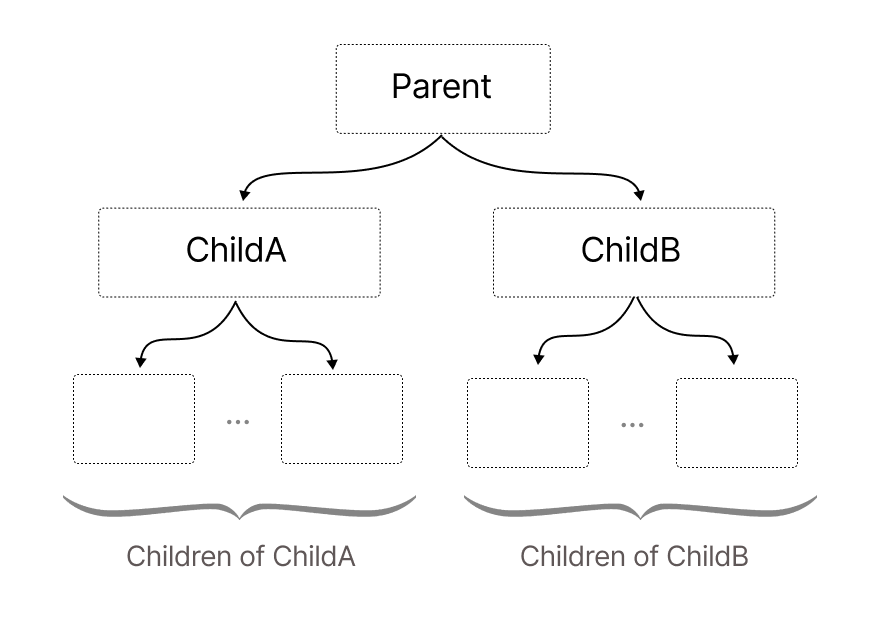
\includegraphics[width=0.5\textwidth]{images/react_parent_child}
    \caption{Tree representation of the created components}
    \label{image_react_tree}
\end{figure}

Up until now, only props have been presented.
Props can be thought of as
immutable data within the scope of a component. Most applications
though, need to have mutable data, also referred to as state, in order
to be interactive.
In class components, state can be achieved with an
initialization in the constructor and the use of the \texttt{setState}
method for state updates.


Following, the usage of state is illustrated with the example of a simple
user interface. Figure~\ref{counter_2}
illustrate the result, where clicking the \textbf{+} button increments the count by one
and clicking \textbf{-} decrements it by one. The current count is
reflected in real time.

\begin{figure}
    \centering
    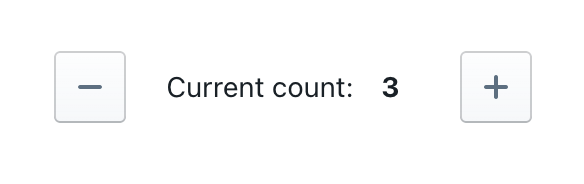
\includegraphics[width=0.5\textwidth]{images/Untitled_1.png}
    \caption{The counter after after clicking \textbf{+} three times.}
    \label{counter_2}
\end{figure}

\begin{figure}
\begin{Shaded}
\begin{Highlighting}[]
\KeywordTok{function} \FunctionTok{Counter}\NormalTok{() \{}
    \KeywordTok{const}\NormalTok{ [count}\OperatorTok{,}\NormalTok{ setCount] }\OperatorTok{=} \FunctionTok{useState}\NormalTok{(}\DecValTok{0}\NormalTok{)}\OperatorTok{;}
    \ControlFlowTok{return }\FunctionTok{\textless{}Container\textgreater{}}
        \FunctionTok{\textless{}Button}
            \OtherTok{icon}\OperatorTok{=}\VariableTok{\{}\StringTok{"minus"}\VariableTok{\}}
            \OtherTok{onClick}\OperatorTok{=}\VariableTok{\{}\NormalTok{() }\KeywordTok{=\textgreater{}} \FunctionTok{setCount}\NormalTok{(count }\OperatorTok{{-}} \DecValTok{1}\NormalTok{)}\VariableTok{\}}
        \FunctionTok{/\textgreater{}}
        \KeywordTok{\textless{}span\textgreater{}}\NormalTok{Current count: }\KeywordTok{\textless{}b\textgreater{}}\VariableTok{\{}\NormalTok{count}\VariableTok{\}}\KeywordTok{\textless{}/b\textgreater{}\textless{}/span\textgreater{}}
        \FunctionTok{\textless{}Button}
            \OtherTok{icon}\OperatorTok{=}\VariableTok{\{}\StringTok{"plus"}\VariableTok{\}}
            \OtherTok{onClick}\OperatorTok{=}\VariableTok{\{}\NormalTok{() }\KeywordTok{=\textgreater{}} \FunctionTok{setCount}\NormalTok{(count }\OperatorTok{+} \DecValTok{1}\NormalTok{)}\VariableTok{\}}
        \FunctionTok{/\textgreater{}}
    \FunctionTok{\textless{}/Container\textgreater{}}
\NormalTok{\}}
\end{Highlighting}
\end{Shaded}
\caption{Implementation of the counter using a function component}
\label{code_counter_function}
\end{figure}

The figure~\ref{code_counter_function} demonstrates the implementation of the counter using a
function, in which \texttt{Counter} is a component that accepts
no props and holds a state. It uses a \texttt{Container} element to
apply a layout and nests in two button components and an \texttt{HTML span}\cite{mozilla_span}.
The button receives an icon name and a callback function to
be called when clicked. The current count is embedded in the text inside
the span using curly braces.

Although state is mutable, it is not to be assigned directly, but rather
by using the method \texttt{setState}, so that React is notified by the
change and can orchestrate the needed UI updates\cite{react_state_and_lifecycle}.

The function \texttt{useState} is one of the many special functions
available by the React API, so called hooks~\cite{react_hooks}.
Hooks are special
functions that start with \texttt{use} and can only be used in function
components or within other hooks. There are other hooks available for
function components and lifecycle methods for class components. These
are left out of this introductory chapter, since they have a low
relevance within the scope of the work. In the following, function components are mainly
used over class components due to their simplicity and their support by
all the selected state management libraries.

\clearpage
\clearpage
\hypertarget{problem-definition}{
\section{Problem Definition}\label{problem-definition}}

Before diving into the different approaches, it is important to identify
what problems SMLs try to solve in the first place. The review of the
developer documentation of the SMLs indicates that the fundamental
problem lies in sharing state between multiple components, which can be
split into four problems:

\begin{itemize}
\tightlist
\item
  \textbf{P1:} Shared state. Although react offers great flexibility on
  the structure of the application tree, it prescribes a
  top-down data flow. Meaning, parent nodes pass data to their children.
  This introduces the challenge of how to share data between nodes that
  are far away from one another in the tree. Figure~\ref{image_shared_state}
  illustrates the challenge of sharing state between the components $C_1$ and $D_5$.
\item
\begin{figure}[h!]
    \centering
    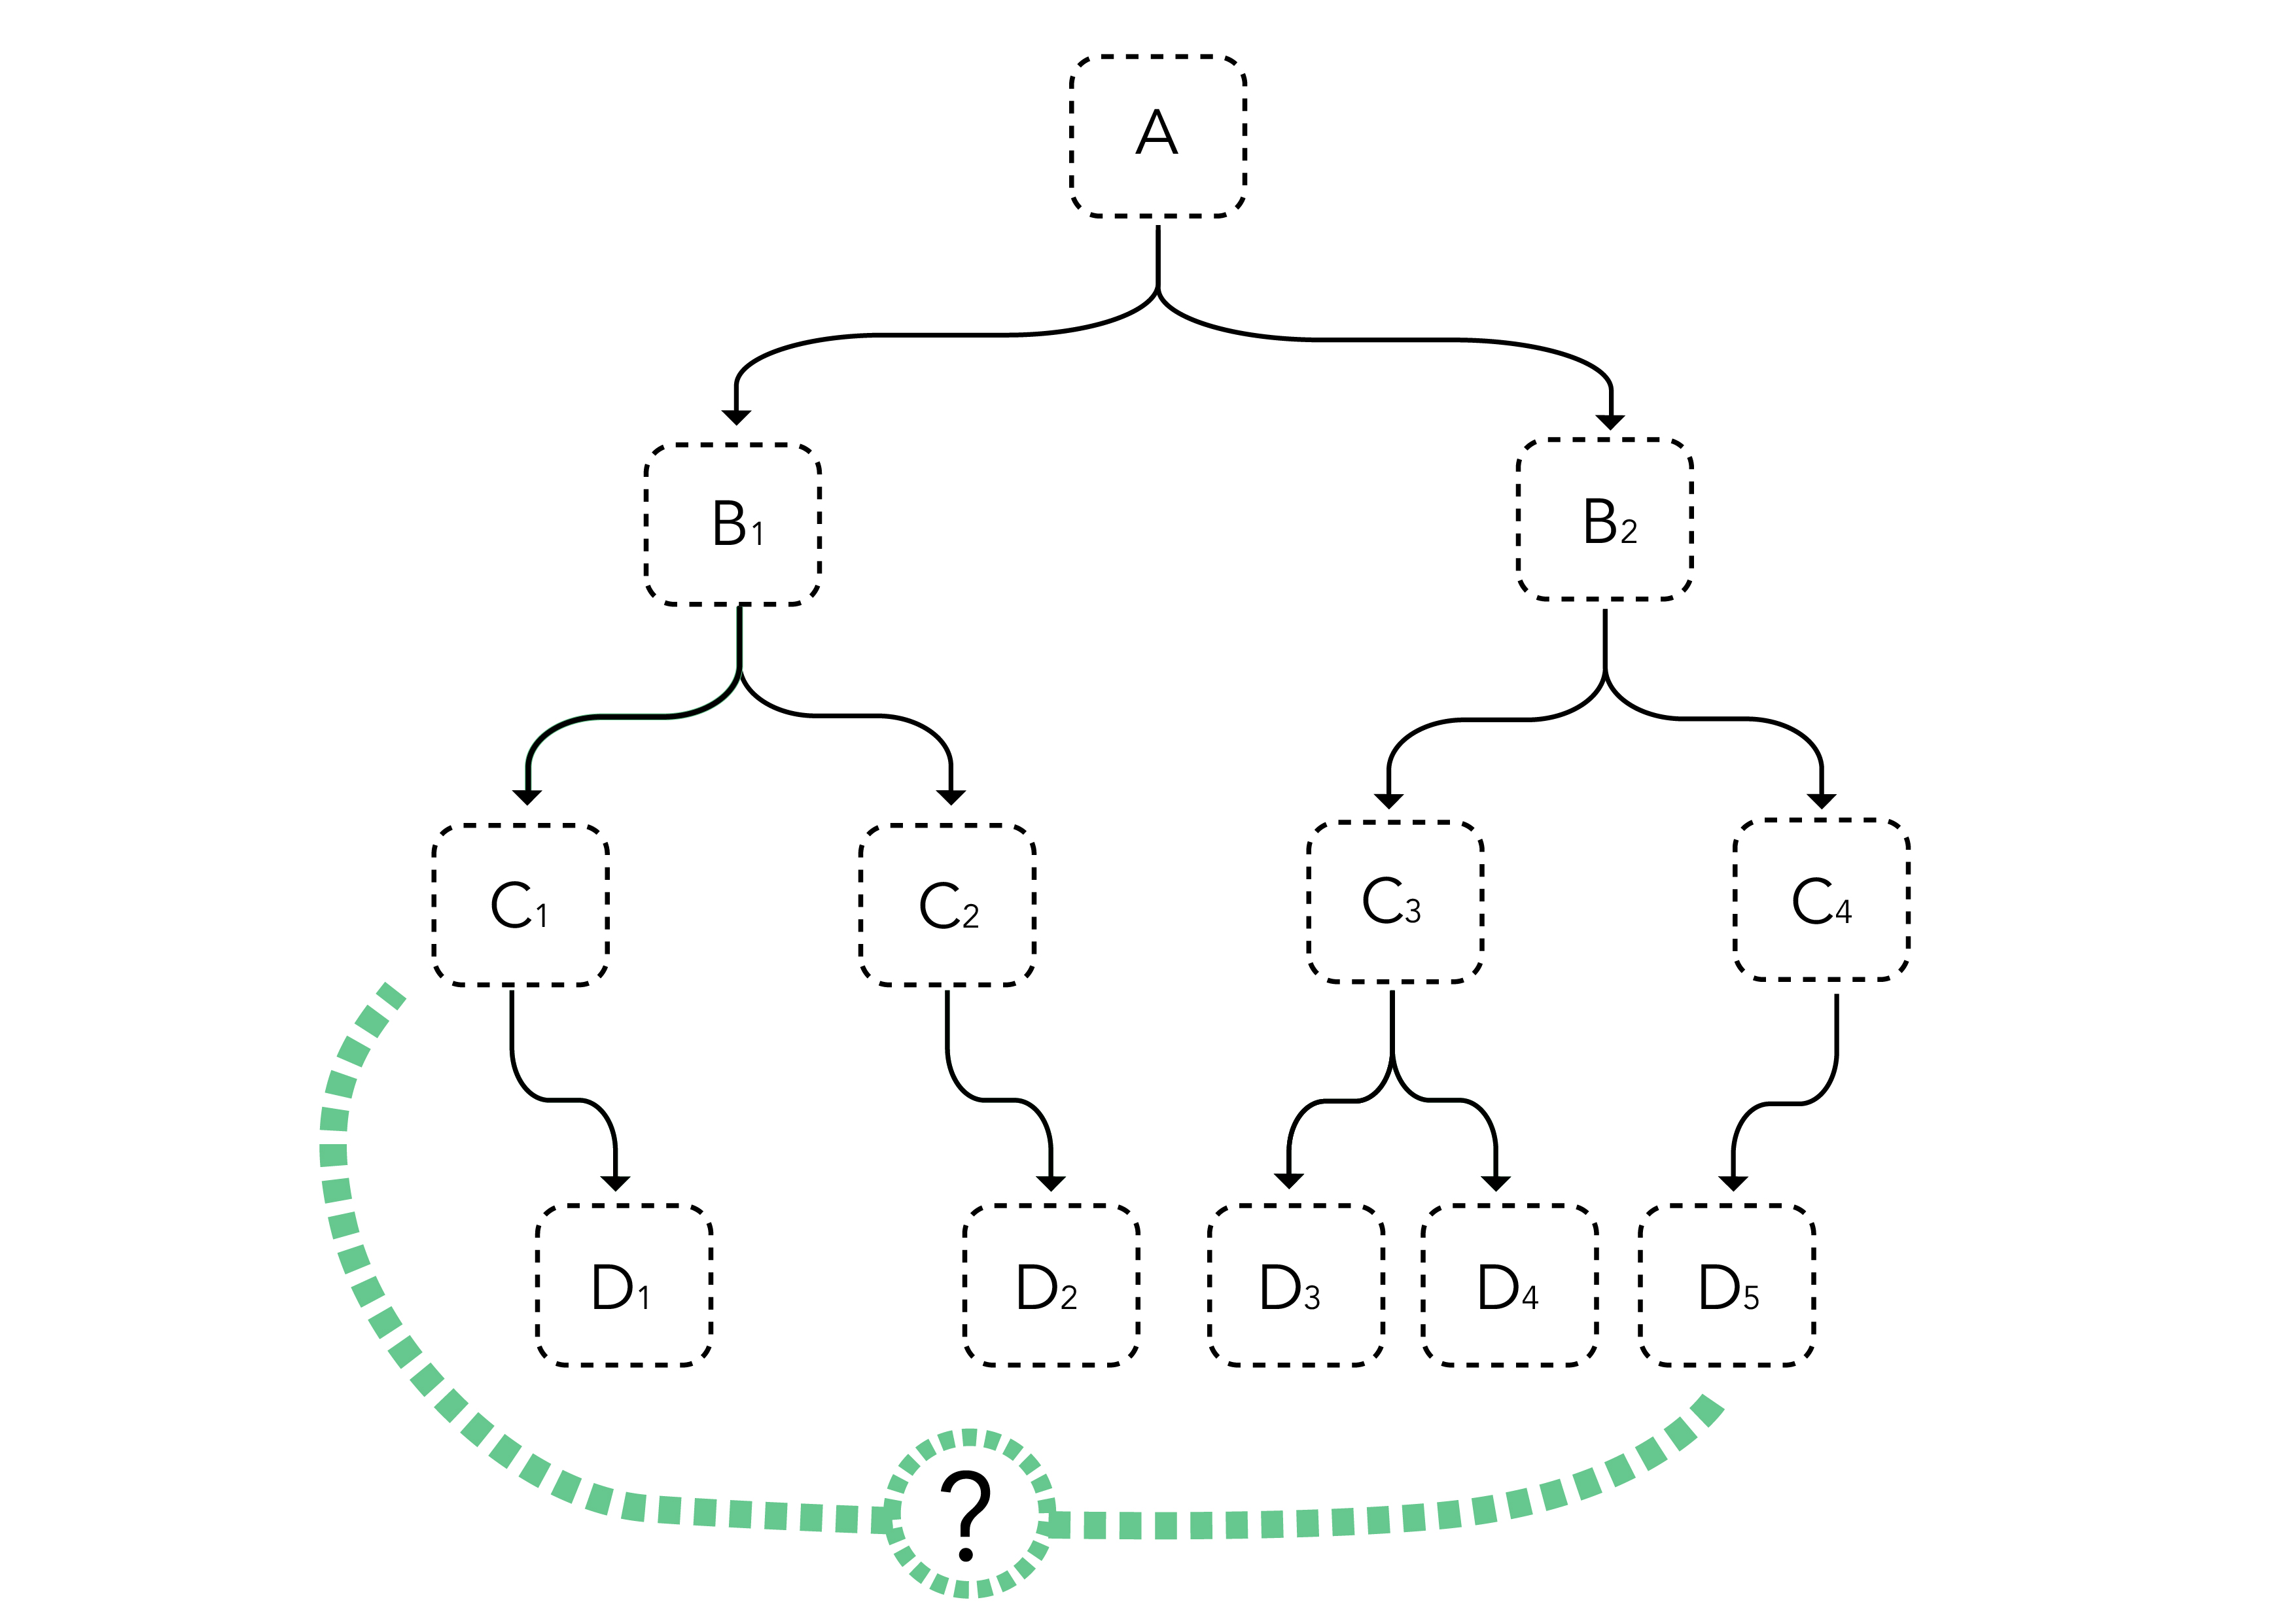
\includegraphics[width=0.7\textwidth]{images/share_state}
    \caption{Example situation illustrating the challenge of shared state}
    \label{image_shared_state}
\end{figure}

  \textbf{P2:} Prop drilling: State needs to be forwarded from higher
  nodes to lower ones that require it, even when intermediate nodes do
  not utilize it. In figure~\ref{image_prop_drilling}, \(D_{3}\) and \(D_6\) both require
  the state \(S\), therefore it is imported in the closest common
  ancestor node \(A\) and propagated throughout the tree. As can be seen
  in the figure, the node \(B_1\), \(B_2\), \(C_2\) and \(C_4\) do not
  use the state, nevertheless they need to forward it.
\begin{figure}[h!]
    \centering
    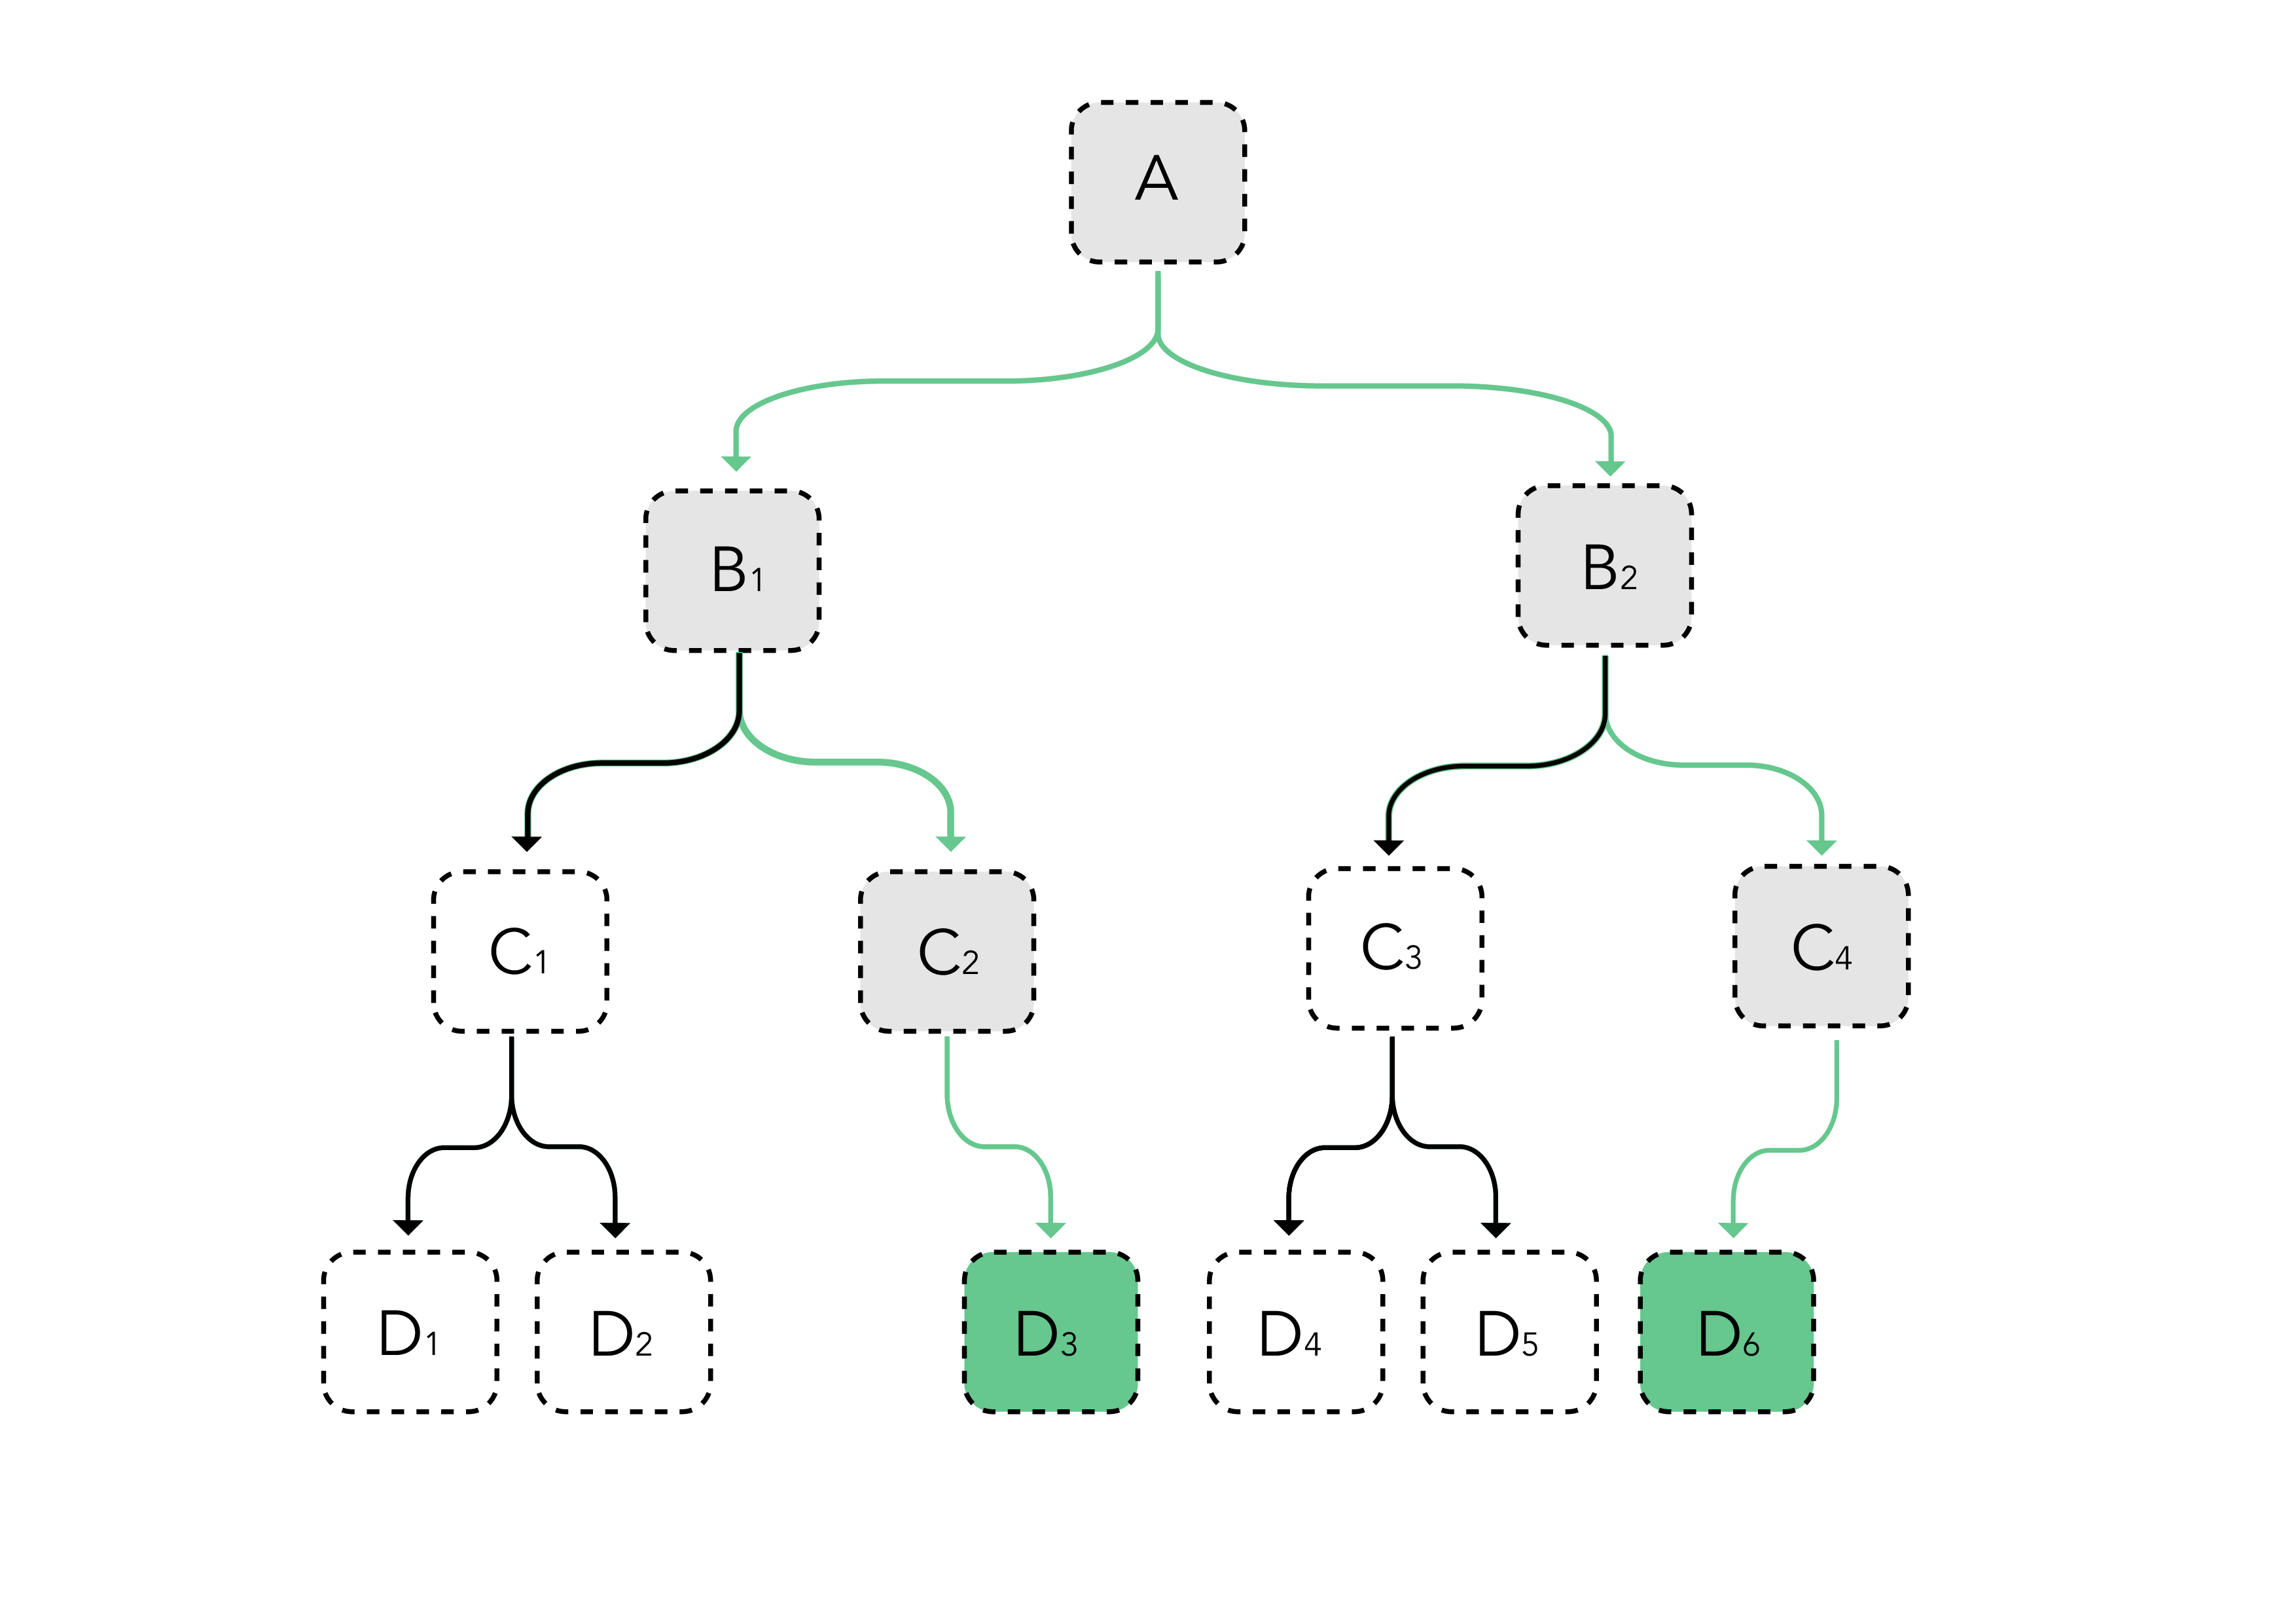
\includegraphics[width=0.7\textwidth]{images/prop_drilling}
    \caption{Example situation illustrating prop drilling}
    \label{image_prop_drilling}
\end{figure}
  Typically the lower
  nodes are \textbf{presentational components}~\cite{presentational_and_container_components}: They
  represent concrete implementations of User Interface elements such as
  text inputs, buttons and checkboxes. On the other hand, higher nodes are
  \textbf{container components:} they contain business logic and use
  presentational components while being agnostic about implementation
  details~\cite{presentational_and_container_components}. For instance, prop drilling becomes apparent,
  when a current application theme that should be passed from the root node
  throughout the application tree, so that the presentational
  components can access it and render accordingly.
\item
\begin{figure}[h!]
    \centering
    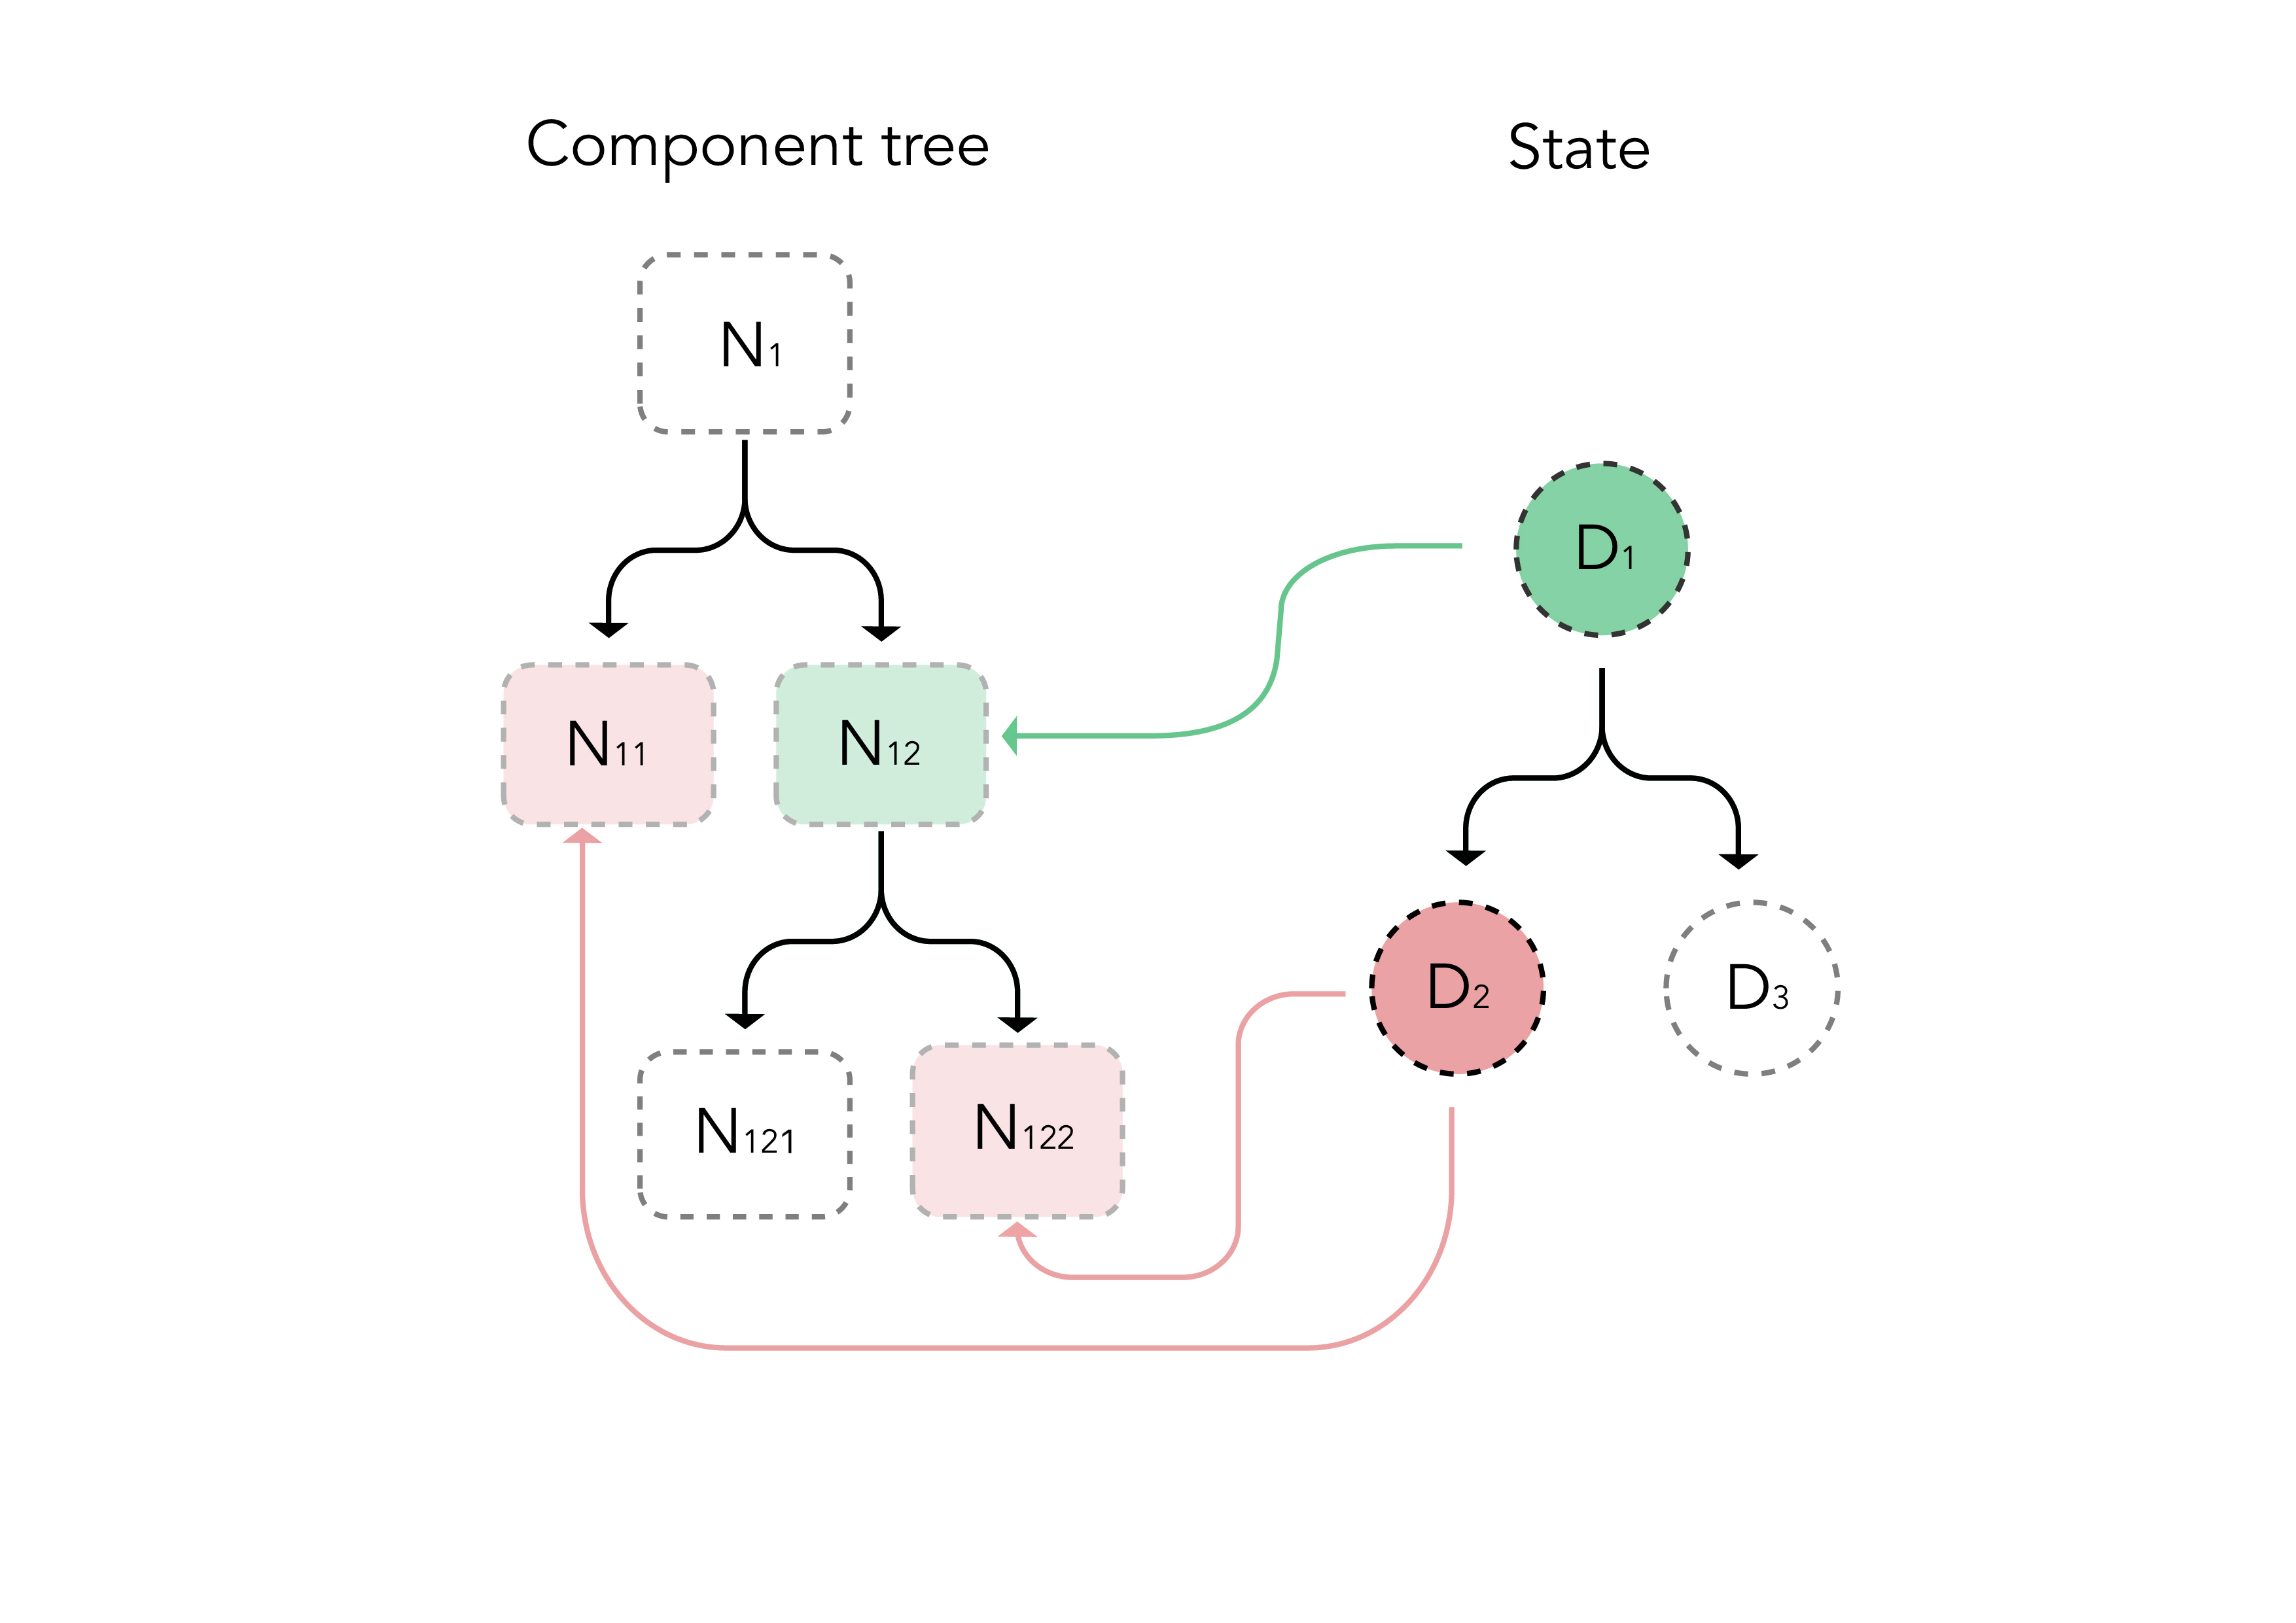
\includegraphics[width=0.7\textwidth]{images/derived_state}
    \caption{Example situation illustrating derived state}
    \label{image_derived_state}
\end{figure}
  \textbf{P3:} State interdependencies/derived state. It is usual in an
  application that multiple states are dependent on others forming a
  state dependency tree. An example of a state dependency tree is depicted in figure~\ref{image_derived_state},
  where \(D_2\) and \(D_3\) depend on \(D_1\). An example for
  this could be: \(D_1\) is the user selection of an element in a list.
  \(D_2\) could be a field in the selected object and \(D_3\) is some
  additional data that needs to be fetched for this specific object.
\item
  \textbf{P4:} Unnecessary re-renderings. When the data of a component
  changes, React re-renders that component and its belonging subtree. In
  a nutshell, React recursively calls \texttt{render} on the
  component and its children and update the Document Object Model (DOM)~\cite{mozilla_dom}
  accordingly (more about this in chapter
  chapter~\ref{reacts-inner-functionality}). This process can be
  exhaustive as it can cause performance problems when one of the
  affected nodes is high in the application tree. Thereby three
  re-rendering performance levels are differentiated: the first as
  \textbf{optimal re-renderings}, where only the nodes whose state changed
  are re-rendered, the second as \textbf{suboptimal re-renderings}, where
  nodes are re-rendered due to their possible change of their derived
  state, and the third as \textbf{redundant re-renderings}, where nodes are
  re-rendered even when their state has not changed.
\end{itemize}

\hypertarget{problem-use-case}{%
\section{Problem Use Case}\label{problem-use-case}}

In the following, a use case incorporating the above mentioned problems
is formulated, that is applied in later steps of this work in the
evaluation of the selected approaches.

\begin{figure}[h!]
\centering
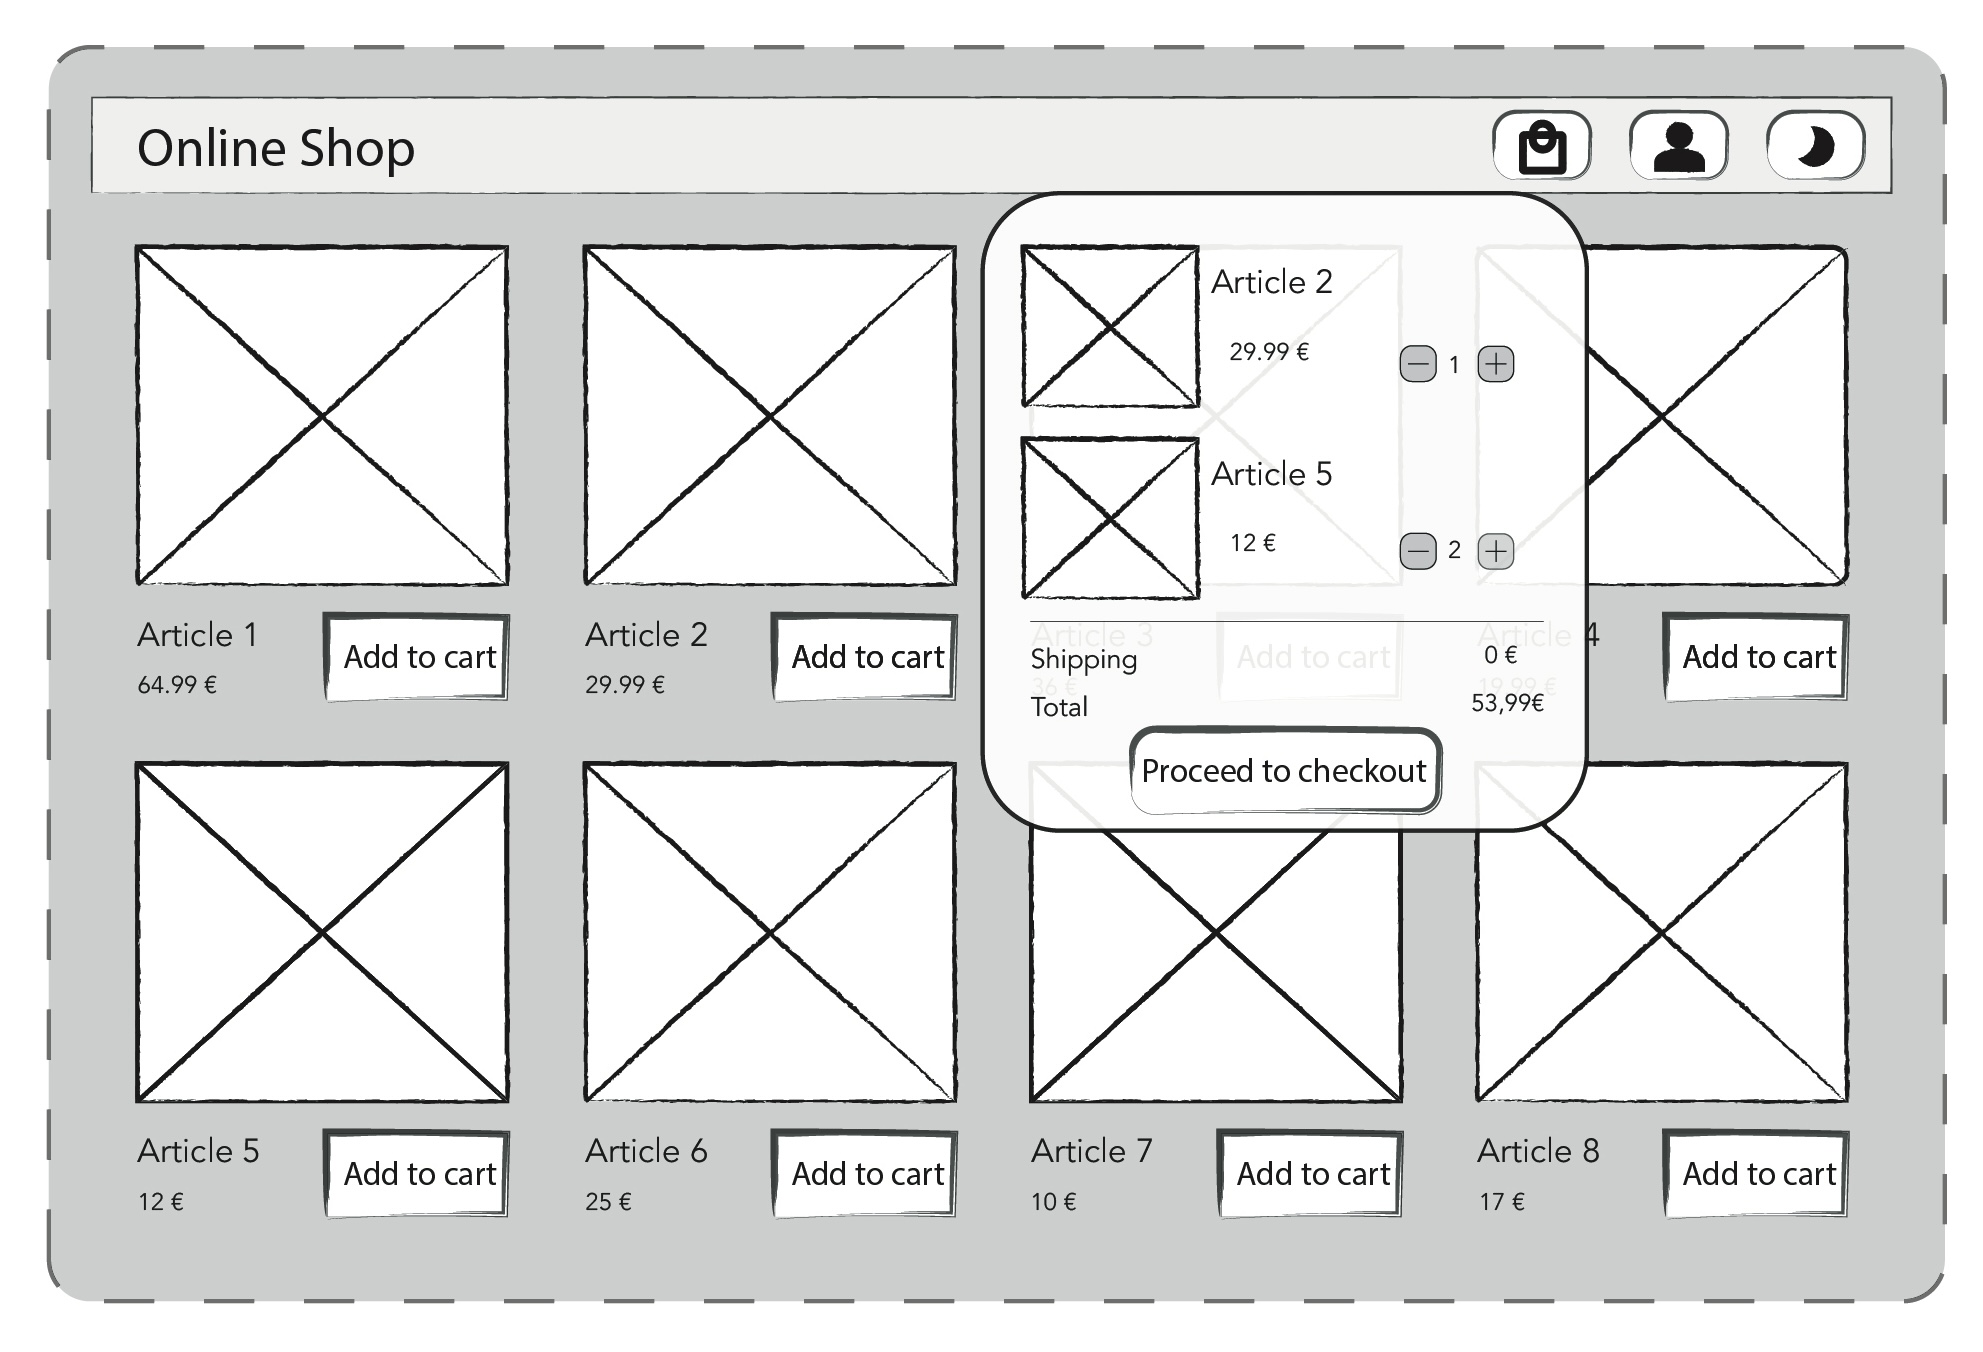
\includegraphics{images/use_case}
\caption{The wireframe of the use case where the cart popup is open}
    \label{image_use_case}
\end{figure}

This use case is an online shop
website, which is depicted in Figure~\ref{image_use_case}.
The displayed articles are fetched from
a backend server and can be added to the cart. The count of the articles
currently in the cart is shown by a badge on the cart icon. This
embodies the problem of derived state (\textbf{P3}). The cart state,
which is also persisted on the backend side can be viewed by clicking on
the cart icon. Since adding items in the cart and the displayed items
happen in different sections of the UI, the problem of
shared state (\textbf{P1}) is therefore included. By adding the possibility to switch between
dark and light mode, which is a common pattern nowadays, the theme needs
to be shared throughout the application, effectively showing the prop
drilling problem (\textbf{P2}). In order to test whether the application
efficiently handles re-renderings (\textbf{P4}), another state is added:
the authenticated user. By clicking on the profile icon, a popup prompts
the user to log in or out. The authenticated user is shown in the
profile icon and popup. Finally, in order to add some business logic, a
free shipping is offered when the total of the cart surpasses a specific amount.

In order to implement the backend functionality, the application needs
to communicate with a backend server. Luckily, this can be easily mocked
by creating a service class in the frontend that offers the same
interface. Mainly, all methods should include a delay and be
asynchronous in order to simulate an implementation using the browsers' built-in \texttt{fetch} function~\cite{mozilla_fetch}.
The functionality offered by the service is described in the 
figure~\ref{table_service_api} below and the used types are shown in figure 
~\ref{image_class_diagram}.

\begin{figure}[h!]
    \small
    \centering
    \begin{tabular}{||p{4cm} p{3.5cm} p{6cm}||}
        \hline
         Method & Returns & Description \\ [0.5ex]
        \hline\hline

        \texttt{getAllArticles()} & \texttt{Promise<Article[]>} & Get all the articles available \\
        \texttt{getCart()} & \texttt{Promise<Cart>} & Get the current cart, including the articles, their respective count, shipping costs and total \\
        \texttt{addArticleToCart (articleId: string)} & \texttt{Promise<Cart>} & Add an article to the cart and return the new cart. \\
        \texttt{removeArticleFromCart (articleId: string)} & \texttt{Promise<Cart>} & Removes an article from the cart and return the new cart. \\
        \texttt{logIn()} & \texttt{Promise<Profile>} & Logs the user in and returns the user details including the first name, the last name and the user’s email address. \\
        \texttt{logOut()} & \texttt{Promise<void>} & Logs the user out. \\ [1ex]
        \hline
    \end{tabular}
\caption{API definition of the needed service.}
\label{table_service_api}
\end{figure}

\begin{figure}[h!]
    \centering
    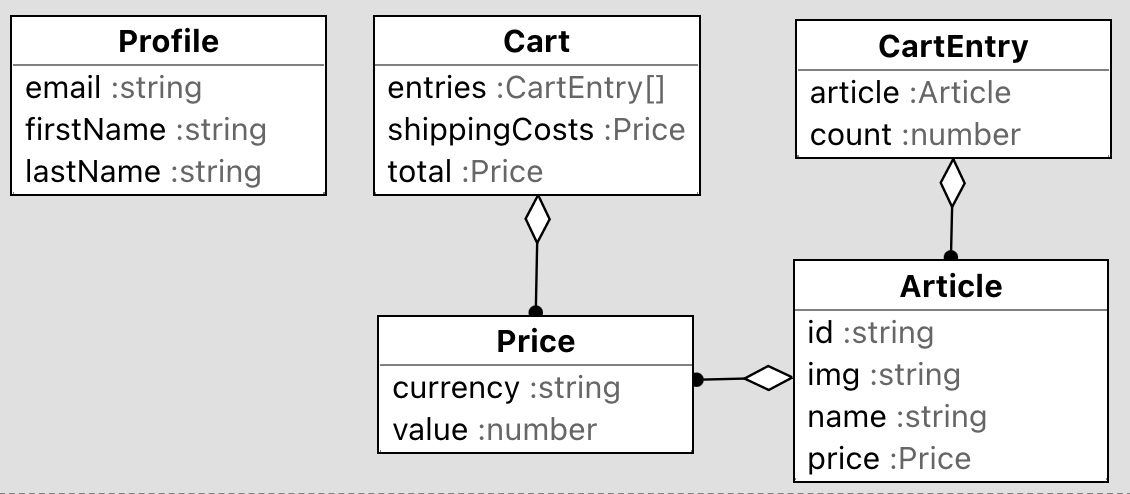
\includegraphics[width=0.8\textwidth]{images/class_diagram}
    \caption{The types used in the API definition of the service}
    \label{image_class_diagram}
\end{figure}

\clearpage
\hypertarget{reacts-inner-functionality}{%
\section{React's
Inner Working}\label{reacts-inner-functionality}}

Thanks to React's declarative API, it is simple to create reactive user
interfaces, which renders correctly when the underlying data changes.
This process of updating the DOM elements is called
Reconciliation~\cite{react_reconciliation}. Reconciliation is based on the concept of the
virtual DOM, where an ideal representation of the UI is kept in memory
and synced with the browser DOM. After each change of
props or state, the DOM needs to be updated to reflect the changes. To
do so, React compares the previous tree with the target tree in a
process referred to as ``diffing''~\cite{react_reconciliation}. Whilst calculating the needed
operations to transform a tree to another one has a complexity of
\(O(n^3)\)~\cite{react_reconciliation}, React uses a heuristic algorithm that achieves a lower
complexity of \(O(n)\). The algorithm makes two basic assumptions that
prove to be valid in almost all practical use cases. The first
assumption is that two nodes of different types produce different trees.
And the second implies, the prop \texttt{key} can be used to define the
identity of a node.

The process of Diffing works as follow: Starting from the root node, the
\texttt{render} method is called and compared with the previous content.
If elements of different types are returned, then the old tree is
removed and replaced with the new one. Otherwise, the attributes are
compared and only the needed changes are made. The algorithm is then
recursively applied to the child components. For example in figure~\ref{code_reconciliation_class_name},
only the prop \texttt{className} needs to be modified. In other words,
when a component is re-rendered, it is not removed from the application
tree and re-mounted. Rather, its \texttt{render} method is called and
the needed changes are calculated.

\begin{figure}
\begin{Shaded}
\begin{Highlighting}[]
\CommentTok{// actual}
\KeywordTok{\textless{}div} \OtherTok{className}\OperatorTok{=}\StringTok{"before"} \OtherTok{title}\OperatorTok{=}\StringTok{"my-title"} \KeywordTok{/\textgreater{}}

\CommentTok{// target}
\KeywordTok{\textless{}div} \OtherTok{className}\OperatorTok{=}\StringTok{"after"} \OtherTok{title}\OperatorTok{=}\StringTok{"my-title"} \KeywordTok{/\textgreater{}}
\end{Highlighting}
\end{Shaded}
\caption{Two nodes to compare that have a different attribute}
\label{code_reconciliation_class_name}
\end{figure}

When recursing on the child components, both lists are simply iterated
over and the needed change operations are computed. For example, when
adding an element to a collection such as in figure~\ref{code_reconciliation_extra_element}, the comparison
of the first two entry sets result in no change needed. Then, upon
arriving at the third element, it becomes apparent that the element
\texttt{\textless{}li\textgreater{}third\textless{}/li\textgreater{}}
need to be added.

\begin{figure}
\begin{Shaded}
\begin{Highlighting}[]
\CommentTok{// actual}
\KeywordTok{\textless{}ul\textgreater{}}
  \KeywordTok{\textless{}li\textgreater{}}\NormalTok{first}\KeywordTok{\textless{}/li\textgreater{}}
  \KeywordTok{\textless{}li\textgreater{}}\NormalTok{second}\KeywordTok{\textless{}/li\textgreater{}}
\KeywordTok{\textless{}/ul\textgreater{}}

\CommentTok{// target}
\KeywordTok{\textless{}ul\textgreater{}}
  \KeywordTok{\textless{}li\textgreater{}}\NormalTok{first}\KeywordTok{\textless{}/li\textgreater{}}
  \KeywordTok{\textless{}li\textgreater{}}\NormalTok{second}\KeywordTok{\textless{}/li\textgreater{}}
  \KeywordTok{\textless{}li\textgreater{}}\NormalTok{third}\KeywordTok{\textless{}/li\textgreater{}}
\KeywordTok{\textless{}/ul\textgreater{}}
\end{Highlighting}
\end{Shaded}
\caption{Two trees to be compared, where the second one has an extra element in the end}
\label{code_reconciliation_extra_element}
\end{figure}


This implementation leads to redundant operations when elements are
added in other places than at the end. For instance, when an element is
added in the beginning the so far presented procedure will
result in changing the content of the two first nodes and adding a third
one.

This issue is solved by using the unique \texttt{key} attribute to
identify the nodes. Figure~\ref{code_reconciliation_usage_of_keys} gives an examples that improves the
previous code.

\begin{figure}
\begin{Shaded}
\begin{Highlighting}[]
\CommentTok{// actual}
\KeywordTok{\textless{}ul\textgreater{}}
  \KeywordTok{\textless{}li} \OtherTok{key}\OperatorTok{=}\StringTok{"2015"}\KeywordTok{\textgreater{}}\NormalTok{Duke}\KeywordTok{\textless{}/li\textgreater{}}
  \KeywordTok{\textless{}li} \OtherTok{key}\OperatorTok{=}\StringTok{"2016"}\KeywordTok{\textgreater{}}\NormalTok{Villanova}\KeywordTok{\textless{}/li\textgreater{}}
\KeywordTok{\textless{}/ul\textgreater{}}

\CommentTok{// target}
\KeywordTok{\textless{}ul\textgreater{}}
  \KeywordTok{\textless{}li} \OtherTok{key}\OperatorTok{=}\StringTok{"2014"}\KeywordTok{\textgreater{}}\NormalTok{Connecticut}\KeywordTok{\textless{}/li\textgreater{}}
  \KeywordTok{\textless{}li} \OtherTok{key}\OperatorTok{=}\StringTok{"2015"}\KeywordTok{\textgreater{}}\NormalTok{Duke}\KeywordTok{\textless{}/li\textgreater{}}
  \KeywordTok{\textless{}li} \OtherTok{key}\OperatorTok{=}\StringTok{"2016"}\KeywordTok{\textgreater{}}\NormalTok{Villanova}\KeywordTok{\textless{}/li\textgreater{}}
\KeywordTok{\textless{}/ul\textgreater{}}
\end{Highlighting}
\end{Shaded}
\caption{Two trees to be compared. The usage of keys indentifies that an element has been added}
\label{code_reconciliation_usage_of_keys}
\end{figure}

\clearpage
\hypertarget{state-management-libraries}{%
\section{State Management
Libraries}\label{state-management-libraries}}

Following, a selection of state management libraries is presented. Two
factors has been taking into consideration when choosing the libraries:
the popularity of the library and the programming paradigm it is based
on. The selected libraries are React Context~\cite{react_context} which falls into
the global state category, Redux Toolkit~\cite{redux_toolkit} which follows a flux
based approach~\cite{flux}, MobX~\cite{mobx} which follows the observable pattern, Recoil
\cite{recoil} which is based on the concept of atomic state, and React Query
\cite{react_query}, a query based approach.

\hypertarget{global-state}{%
\subsection{Global State}\label{global-state}}

Built into React, React Context provides the possibility of sharing a
piece of state in a defined context. The usage of React Context requires
the creation of a context object and a context provider. As the name
suggests, the context provider holds the actual state that is shared
with the consumers. Its usage in the component tree defines the scope
of the context by wrapping a part of the component tree. All the
descendent components of the provider have access to the shared state
through the use of the hook \texttt{useContext}. Figure~\ref{code_example_of_react_context} shows the
creation and usage of a context globally. It is to be noted, that there
is usually a one-to-many relation between context providers and
consumers, although multiple providers can be used to overwrite values
deeper in the components tree~\cite{react_context}.

\begin{figure}
\begin{Shaded}
\begin{Highlighting}[]
\NormalTok{// Context creation}
\NormalTok{const MyContext = createContext();}

\NormalTok{// Creating the context provider}
\NormalTok{export const MyContextProvider = (\{}
\NormalTok{    children,}
\NormalTok{\}) =\textgreater{} \{}
\NormalTok{    const [state, setState] = useState(/* initial state */);}
\NormalTok{    return} (
\NormalTok{        \textless{}MyContext.Provider value=\{\{ state, setState \}\}\textgreater{}}
\NormalTok{            \{children\}}
\NormalTok{        \textless{}/MyContext.Provider\textgreater{}}
\NormalTok{    );}
\NormalTok{\};}

\NormalTok{// usage in a consumer component}
\NormalTok{export const \{ state, setState \} = useContext(MyContext)}
\end{Highlighting}
\end{Shaded}
\caption{Example usage of React Context.}
\label{code_example_of_react_context}
\end{figure}

When using React Context, the consumer components become functions that
contain implicit parameters that are not declared in their signatures.
This means that they behave differently depending on the context they
are called from. React Context is therefore considered as a form of
dynamic scoping, where the variable binding (the association of a
variable to its actual value) happens dynamically~\cite{dynamic_scoping}.
According to~\cite{dynamic_scoping}, ``this allows for a number of well-known benefits
[...], like conciseness, modularity and adaptability''. When having a
unique provider shared throughout the application however, React Context
can be interpreted as a form of global state.

\clearpage
\clearpage
\hypertarget{flux-based-state-management-libraries}{%
\subsection{Flux-Based State Management
Libraries}\label{flux-based-state-management-libraries}}

One of the popular state management libraries is Redux~\cite{redux}. It has
gained popularity since it drew from Flux pattern, a pattern that has
been recommended for React~\cite{flux_recommendation}. An
application using the flux pattern is made up of three main components
shown in figure~\ref{image_redux_simple}:

\begin{itemize}
\tightlist
\item
  The~\textbf{state}, the single source of truth that drives the
  application,
\item
  The~\textbf{view}, a set of UI components that renders based on the
  current state, and
\item
  The~\textbf{actions}, the events that occur in the application based
  on user interaction, and trigger updates in the state.
\end{itemize}

\begin{figure}
\centering
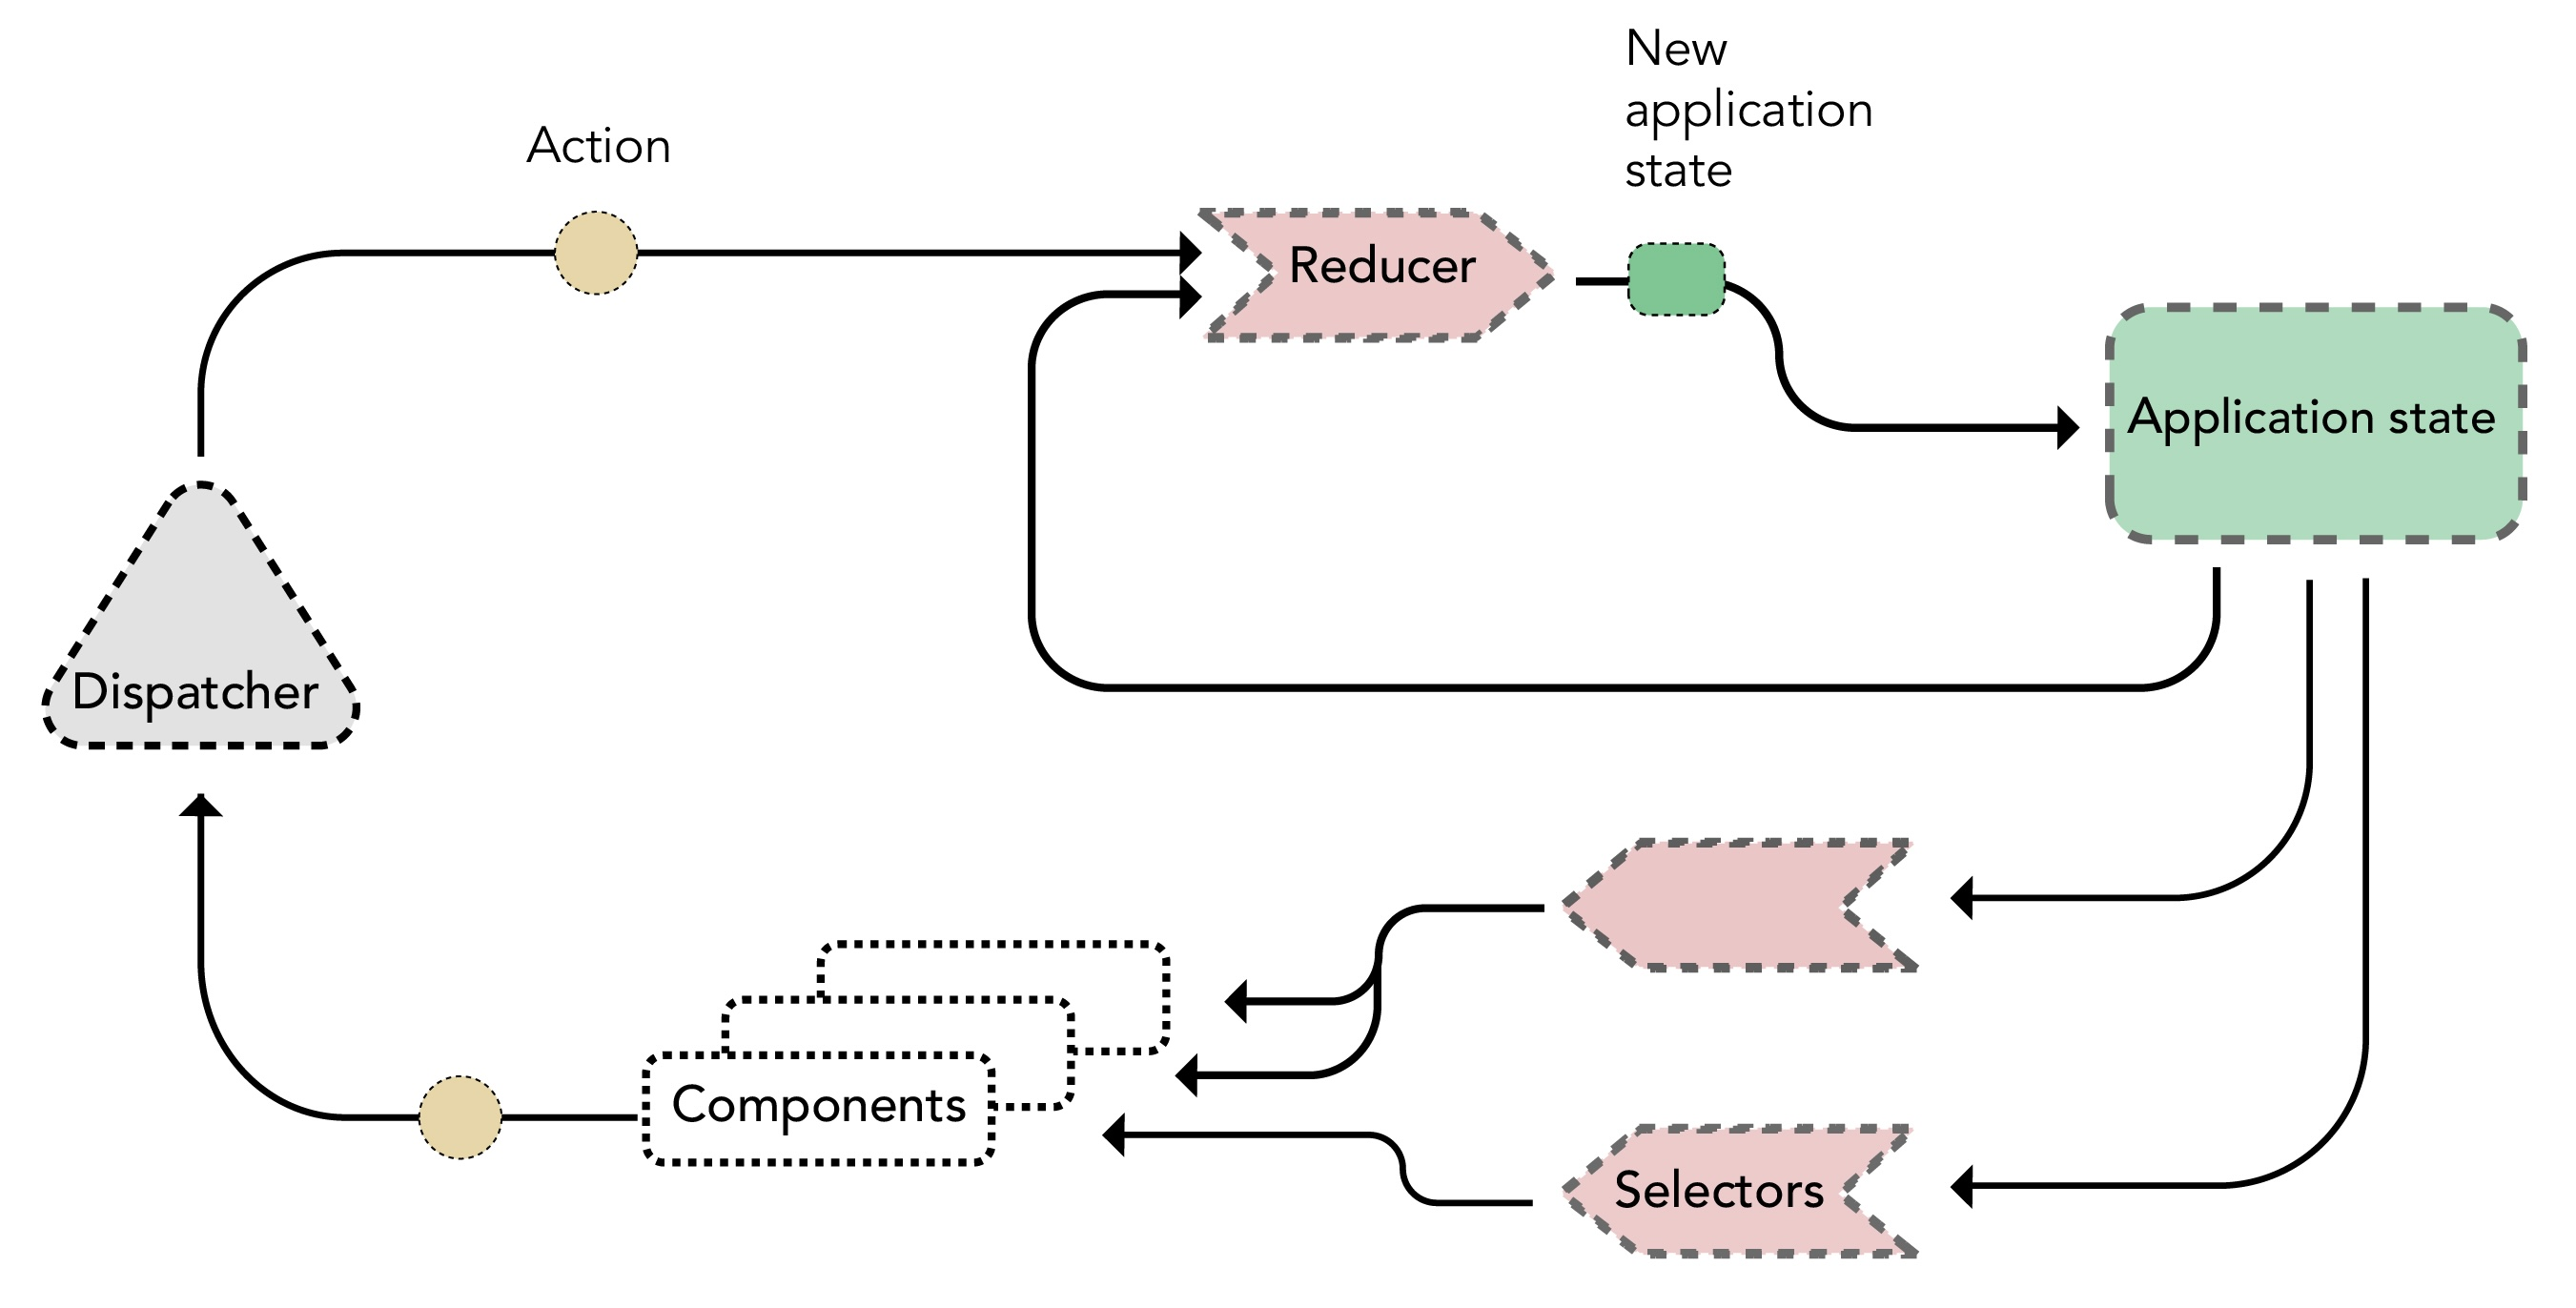
\includegraphics{images/redux}
\caption{The components of an application using Redux}
\label{image_redux_simple}
\end{figure}

This definition of the paradigm enforces a one way data flow, meaning
that the application state cannot be changed directly, but through
actions, which leads to more predictability. Actions are nothing more
that a JavaScript object containing a type that typically follows the
pattern \texttt{"domain/eventName"} along with a \texttt{payload} field
containing other parameters. Figure~\ref{code_action_and_action_creator} shows a simple action
and a dynamic action creator.

\begin{figure}[h!]
\begin{Shaded}
\begin{Highlighting}[]
\CommentTok{// a constant action}
\KeywordTok{const}\NormalTok{ addTodoAction }\OperatorTok{=}\NormalTok{ \{}
  \DataTypeTok{type}\OperatorTok{:} \StringTok{\textquotesingle{}todos/add\textquotesingle{}}\OperatorTok{,}
  \DataTypeTok{payload}\OperatorTok{:} \StringTok{\textquotesingle{}Buy milk\textquotesingle{}}
\NormalTok{\}}

\CommentTok{// a dynamic action creator where the payload is parameterized}
\KeywordTok{const}\NormalTok{ createAddTodoAction }\OperatorTok{=}\NormalTok{ (payload) }\KeywordTok{=\textgreater{}}\NormalTok{ (\{}
  \DataTypeTok{type}\OperatorTok{:} \StringTok{\textquotesingle{}todos/add\textquotesingle{}}\OperatorTok{,}
\NormalTok{  payload}
\NormalTok{\})}
\end{Highlighting}
\end{Shaded}
\caption{Examples of an action and an action creator}
\label{code_action_and_action_creator}
\end{figure}

When an action is dispatched, it is passed to a \textbf{reducer}
function along with the old state and returns the new one. Figure~\ref{code_todo_redux}
shows an example of a todos application. The list of todos that is
initially empty is extended when the action with the type
\texttt{todos/add} is dispatched. It is to be noted, that reducers are
pure functions, meaning that the output of the function depends strictly
in the provided parameters.

\begin{figure}
\begin{Shaded}
\begin{Highlighting}[]
\KeywordTok{function} \FunctionTok{todosReducer}\NormalTok{(state }\OperatorTok{=}\NormalTok{ \{ }\DataTypeTok{todos}\OperatorTok{:}\NormalTok{ [] \}}\OperatorTok{,}\NormalTok{ action) \{}
  \CommentTok{// Check to see if this reducer cares about this action}
  \ControlFlowTok{if}\NormalTok{ (action}\OperatorTok{.}\AttributeTok{type} \OperatorTok{===} \StringTok{\textquotesingle{}todos/add\textquotesingle{}}\NormalTok{) \{}
    \CommentTok{// If so, add a new todo item}
    \ControlFlowTok{return}\NormalTok{ \{}
      \DataTypeTok{todos}\OperatorTok{:}\NormalTok{ [}
                \OperatorTok{...}\NormalTok{state}\OperatorTok{.}\AttributeTok{todos}\OperatorTok{,}
\NormalTok{              \{ }
                    \DataTypeTok{name}\OperatorTok{:}\NormalTok{ action}\OperatorTok{.}\AttributeTok{payload}\OperatorTok{,}
                    \DataTypeTok{checked}\OperatorTok{:} \KeywordTok{false}\OperatorTok{,}
                    \DataTypeTok{id}\OperatorTok{:} \FunctionTok{getNewId}\NormalTok{()}
\NormalTok{                \}}
\NormalTok{    \}}
\NormalTok{  \}}
  \ControlFlowTok{return}\NormalTok{ state}
\NormalTok{\}}
\end{Highlighting}
\end{Shaded}
\caption{Example of a Redux reducer used in a todos application}
\label{code_todo_redux}
\end{figure}

Since the team behind Redux strongly recommends the usage of the
library Redux Toolkit~\cite{redux_style_guide}, it is selected in this work. Redux Toolkit
provides an improved API that addresses a few disadvantages of Redux, mainly the big amount of
boilerplate code and the difficulty of configuring a Redux store
\cite{why_redux_toolkit}. Most notably, the actions and action creators can be generated 
by the library. Redux Toolkit also introduces the concept of slices~\cite{redux_toolkit_slice} which are units of
state with a specific domain that can be combined to create the root
state~\cite{redux_toolkit_configure_store}. Each slice contains the state, reducers, and action
creators.
Additionally, Redux Toolkit simplifies the creation of async actions~\cite{redux_toolkit_async},
that include a loading state and a success or failure result with the
provided function \texttt{createAsyncThunk}~\cite{redux_toolkit_create_async_thunk}.

Before moving to observable state management libraries, it is worth
mentioning that Redux was inspired not only by the original flux
paradigm~\cite{flux}, but also Command Query
Responsibility Segregation (CQRS) and Event
Sourcing~\cite{redux_motivation}.
In a nutshell, CQRS is a pattern that encourages splitting the
application models into separate models for update and
display~\cite{cqrs}. To quote~\cite{cqrs}:

``At its heart is the notion that you can use a different model to
update information than the model you use to read information''.

This is analogous to Redux Toolkit's selectors and action creators.
Figure~\ref{image_without_cqrs} shows an application not using CQRS
and figure~\ref{image_with_cqrs} one that does.

\begin{figure}
\centering
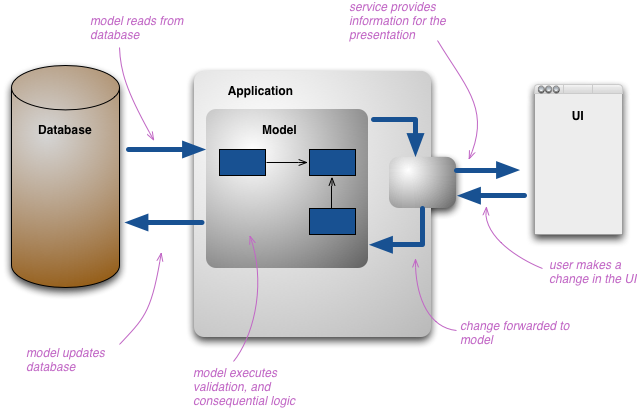
\includegraphics[width=0.7\textwidth]{images/Untitled_9.png}
\caption{Example of an application not using Command Query
Responsibility Segregation (CQRS). Reproduced from~\cite{cqrs}}
\label{image_without_cqrs}
\end{figure}

\begin{figure}
\centering
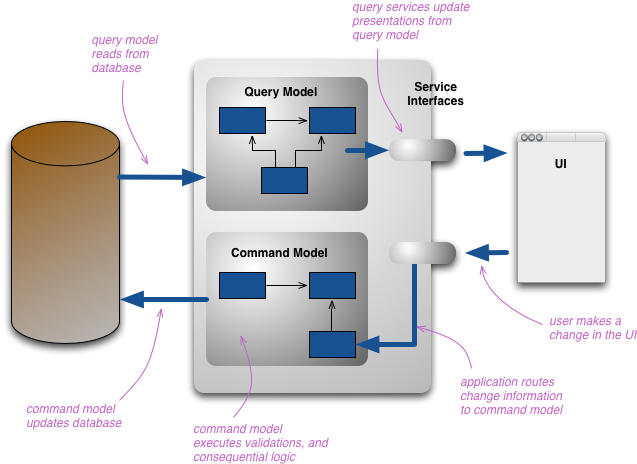
\includegraphics[width=0.7\textwidth]{images/Untitled_10.png}
  \caption{Example of an application using Command Query
  Responsibility Segregation (CQRS). Reproduced from~\cite{cqrs}}
  \label{image_with_cqrs}
\end{figure}

Event sourcing on the other hand, aims to make the changes of the
application state transparent. This is achieved by having events (or
commands) for each change to the application state~\cite{event_sourcing}. In order to
obtain the actual application state, the events must be applied. The
main benefits of this pattern lie in the possibility to trace the
changes of the application state and to reconstruct past states.

\clearpage
\clearpage
\hypertarget{observable-state-management-libraries}{%
\subsection{Observable-Based State Management
Libraries}\label{observable-state-management-libraries}}

MobX is a simple library based on the observer pattern~\cite{gang_of_four},
that hides multiple implementation details. Using the terminology of the
observer pattern, the state of the application constitutes the
``Subject'' whereas the components that use the state are the
``Observers''~\cite{gang_of_four}.
In order to create Observables, the provided function
\texttt{makeAutoObservable()} needs to be called in
the constructor of a class, then an instance can be created
and used
anywhere needed. Each component that uses the created state
is wrapped with \texttt{observer()}. Consequently, each change
made to the state object implicitly causes the notification
of all subscribers.

Compared to the original observer pattern depicted in figure~\ref{image_class_diagram_observer_gof},
MobX offers a minimalistic interface. The logic behind emitting and
listening to events is hidden behind a general interface.

\begin{figure}
\centering
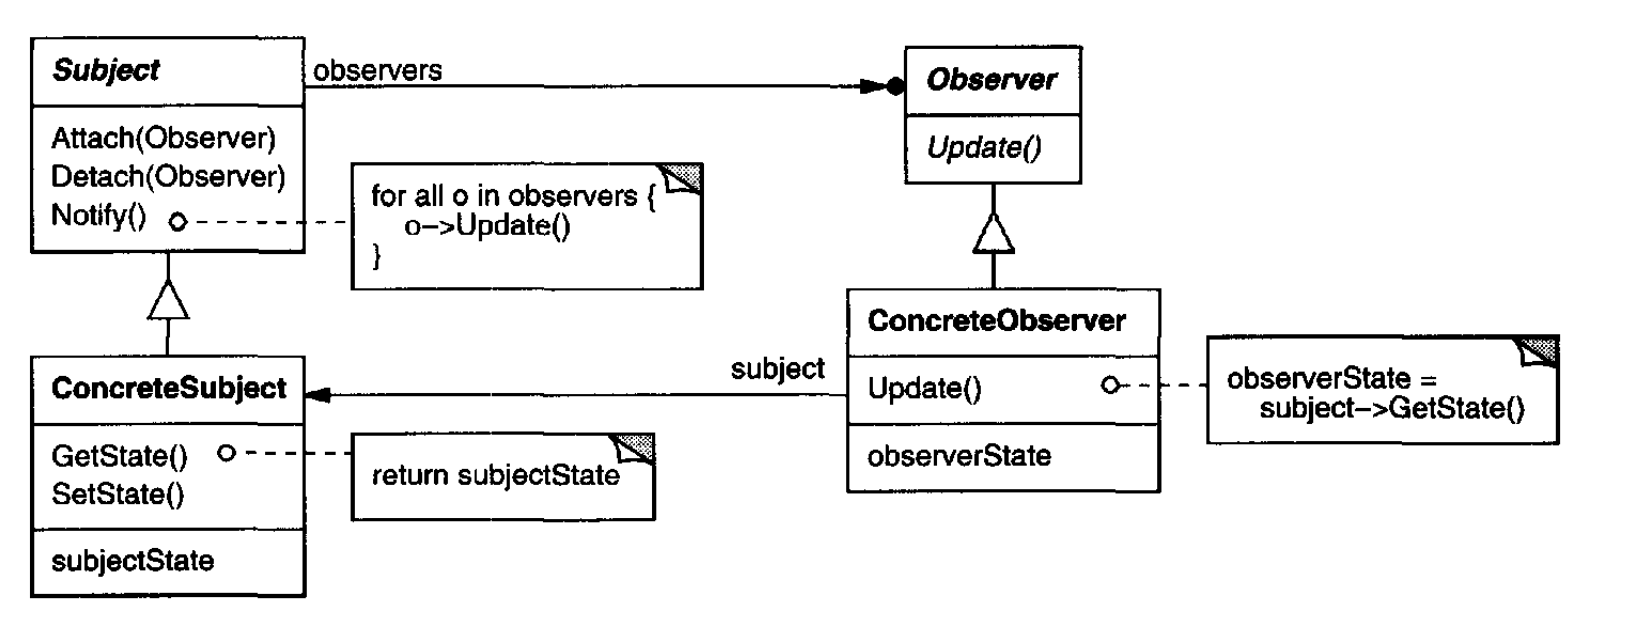
\includegraphics[width=0.8\textwidth]{images/Untitled_11.png}
\caption{Structure of the Observer Pattern. Reproduced from~\cite{gang_of_four}}
\label{image_class_diagram_observer_gof}
\end{figure}


MobX's user documentation refers to this as ``transparently applying
functional reactive
programming''(TFRP)~\cite{mobx}.
Transparent in TFRP refers to the fact, that connecting the observables
to the observers requires ``no explicit wiring''~\cite{tfrp_explanaition}. MobX is considered Reactive because changes in the
observables emit the correct events efficiently, without excessive
events or polling~\cite{tfrp_explanaition}. The functional programming aspect comes from the
possibility to ``apply transformations on input [observable] data and produce output values''\cite{tfrp_explanaition}.

The usage of Functional Reactive Programming, according to~\cite{deprecating_the_observer_pattern},
addresses many of the software engineering principles that the classical
observer pattern violates, which are ``Uniformity and
abstraction'', ``Encapsulation'', ``Resource management'', ``Side-effects'',
``Composability'', ``Separation of concerns'', ``Scalability'' and ``Semantic
distance''~\cite{deprecating_the_observer_pattern}.

\clearpage
\clearpage
\hypertarget{atomic-state-management-libraries}{%
\subsection{Atom-Based State Management
Libraries}\label{atomic-state-management-libraries}}

Recoil~\cite{recoil} is a state management library that takes a different approach on
modeling the application state. In contrast to the previously presented
approaches that are based on a centralized application state, Recoil
offers a distributed state approach by introducing the concept of atoms~\cite{recoil_atoms}
and selectors~\cite{recoil_selectors}. An atom is simply a unit of state, whereas a
selector is a special function that derives its states from one or more
atoms or selectors. This allows the creation of a complex
application state tree, where a changing atom leads to the
re-evaluation of all the dependents~\cite{recoil_core_concepts}.

Figure~\ref{code_recoil_atom_example} illustrates the API provided by Recoil by using an example.
In the example, an atom called counter is defined along with a selector
that returns the value of the counter times ten. The usage in React
components is straightforward, since the method signature resembles
React's built-in \texttt{useState} hook~\cite{react_using_the_state_hook}.

\begin{figure}
\begin{Shaded}
\begin{Highlighting}[]
\CommentTok{// atom definition}
\KeywordTok{const}\NormalTok{ counter }\OperatorTok{=} \FunctionTok{atom}\NormalTok{(\{}
  \DataTypeTok{key}\OperatorTok{:} \StringTok{\textquotesingle{}counter\textquotesingle{}}\OperatorTok{,} \CommentTok{// gloabally unique identifier}
  \ControlFlowTok{default}\OperatorTok{:} \DecValTok{0}\OperatorTok{,} \CommentTok{// the initial value}
\NormalTok{\})}\OperatorTok{;}

\CommentTok{// a selector that computes the value of the counter times ten}
\KeywordTok{const}\NormalTok{ counterTimesTen }\OperatorTok{=} \FunctionTok{selector}\NormalTok{(\{}
  \DataTypeTok{key}\OperatorTok{:} \StringTok{\textquotesingle{}counterTimesTen\textquotesingle{}}\OperatorTok{,}
  \DataTypeTok{get}\OperatorTok{:}\NormalTok{ (\{get\}) }\KeywordTok{=\textgreater{}}  \FunctionTok{get}\NormalTok{(counter) }\OperatorTok{*} \DecValTok{10}
\NormalTok{\})}\OperatorTok{;}

\CommentTok{// usage in a React function component}
\KeywordTok{const}\NormalTok{ [count}\OperatorTok{,}\NormalTok{ setCount] }\OperatorTok{=} \FunctionTok{useRecoilState}\NormalTok{(counter)}\OperatorTok{;}
\end{Highlighting}
\end{Shaded}
\caption{Defining and using state by means of an atom}
\label{code_recoil_atom_example}
\end{figure}

\clearpage
\clearpage
\hypertarget{query-based-state-management-libraries}{%
\subsection{Query-Based State Management
Libraries}\label{query-based-state-management-libraries}}

The last selected approach is the query based state management libraries
represented by the library React Query\cite{react_query}. Although including this approach
as an SML is questionable, it is still taken into account, since it
serves the objectives of this work nonetheless.

React Query's purpose is to manage server state on the client
\cite{react_query_overview} by solving common
problems including caching, grouping multiple requests for the same data
into a single request, detecting and updating out-of-date data in the
background, managing memory and garbage collection of server state,
pagination, and lastly lazy loading data~\cite{react_query_overview}.
Although the library has various features to offer, caching seems to be
the most relevant one since it allows sharing state across different
components. Figures~\ref{image_cache_not_found} and~\ref{image_cache_found} show a simple caching situation where two
components need to access the same information that is stored on a
server. When the first component requires the data, it is fetched from
the server, but when consecutive components require the same data, it is
taken directly from the cache.

\begin{figure}
\centering
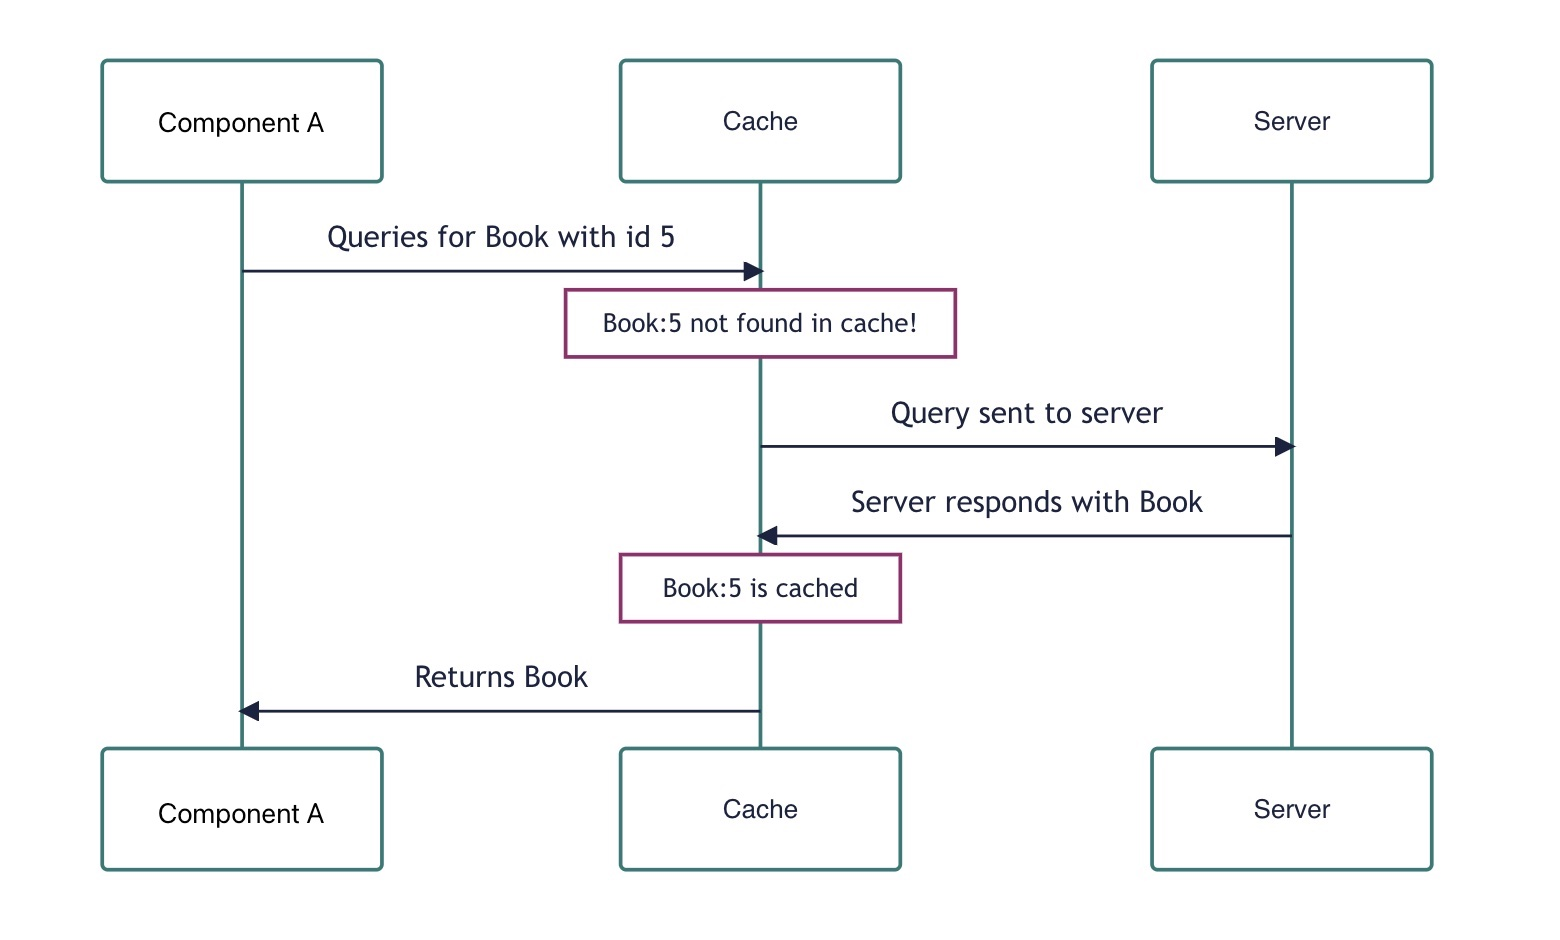
\includegraphics[width=0.7\textwidth]{images/Untitled.jpeg}
\caption{When the first component requires the data, it is queried from the server and saved in the cache}
\label{image_cache_not_found}
\end{figure}

\begin{figure}
\centering
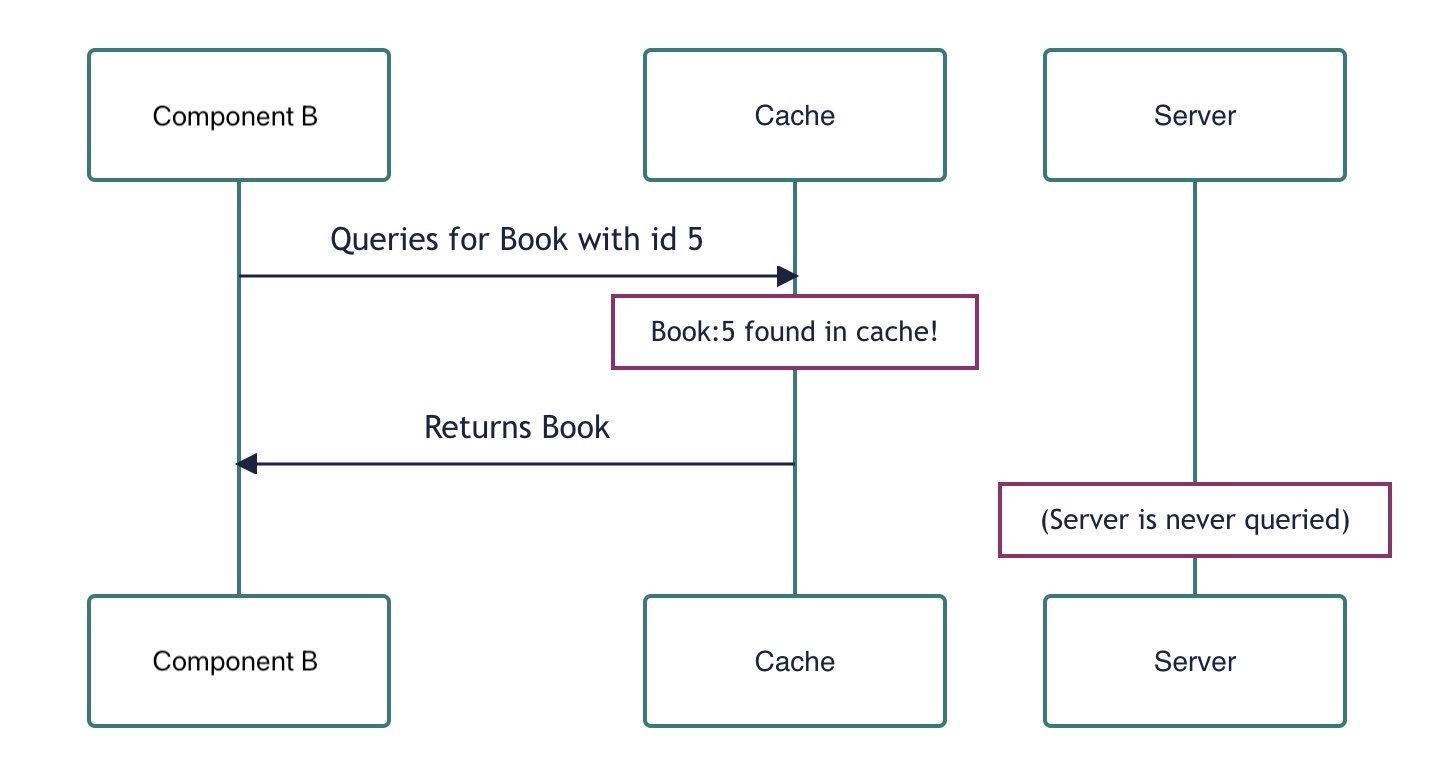
\includegraphics[width=0.7\textwidth]{images/Untitled_1.jpeg}
\caption{When a second component requires the data it is taken from the cache}
\label{image_cache_found}
\end{figure}

The possibility of interacting with the cache also introduces
practicable advantages. For example, when the client performs a mutation
that leads to a changed state, the respective cache can be invalidated. This
means, that by the next time the data is required, it is fetched
from the server. Another use-case which is relevant nowadays is the
topic of ``optimistic updates''~\cite{react_query_optimistic_updates}. ``Optimistic updates''
contribute to a more responsive user experience by displaying applied
changes to the user before they are accepted by the backend server. This can be
easily achieved by overwriting the relevant cache entry manually, since
changes in the cache are reflected instantaneously in the components.
Figure~\ref{code_react_query_use_query} displays an example usage of the library in a component,
where a selection of fields is deconstructed~\cite{mozilla_deconstructing}.

\begin{figure}
\begin{Shaded}
\begin{Highlighting}[]
\NormalTok{const \{}
\NormalTok{        // the data that has been fetched, originally undefined}
\NormalTok{        data,}
\NormalTok{        // if applicable, the error thrown by fetchTodoList}
\NormalTok{        error,}
\NormalTok{        failureCount,}
\NormalTok{        // the status of the query: one of \textquotesingle{}loading\textquotesingle{}, \textquotesingle{}error\textquotesingle{} and \textquotesingle{}success\textquotesingle{}}
\NormalTok{        status,}
\NormalTok{        // a function to manually refetch the query}
\NormalTok{        refetch,}
\NormalTok{        // a function to remove the query from the cache}
\NormalTok{        remove,}
\NormalTok{\} = useQuery(}
\NormalTok{                        [\textquotesingle{}todos\textquotesingle{}], // query keys used for caching}
\NormalTok{                        fetchTodoList // the function used to fetch the data}
\NormalTok{)}
\end{Highlighting}
\end{Shaded}
\caption{Example usage of React Query with deconstructed relevant fields}
\label{code_react_query_use_query}
\end{figure}

\clearpage
\hypertarget{software-quality-models}{%
\chapter{Software quality models}\label{software-quality-models}}

In order to evaluate and compare the different software solutions
mentioned in the previous chapter, it is important to determine the
requirements they should fulfill i.e.~an adequate ``software quality
model''. The following chapter introduces software quality
models, including the definition of the term and an overview on
different models available along with their strengths and weaknesses, and a
special focus is put on the ISO/IEC 25010 Model. Furthermore, requirements
for software quality models are presented based on the
Definition-Assessment-Prediction classification~\cite{dap_model} and Open Source
Software Quality Models are compared.

\begin{figure}[h!]
    \centering
    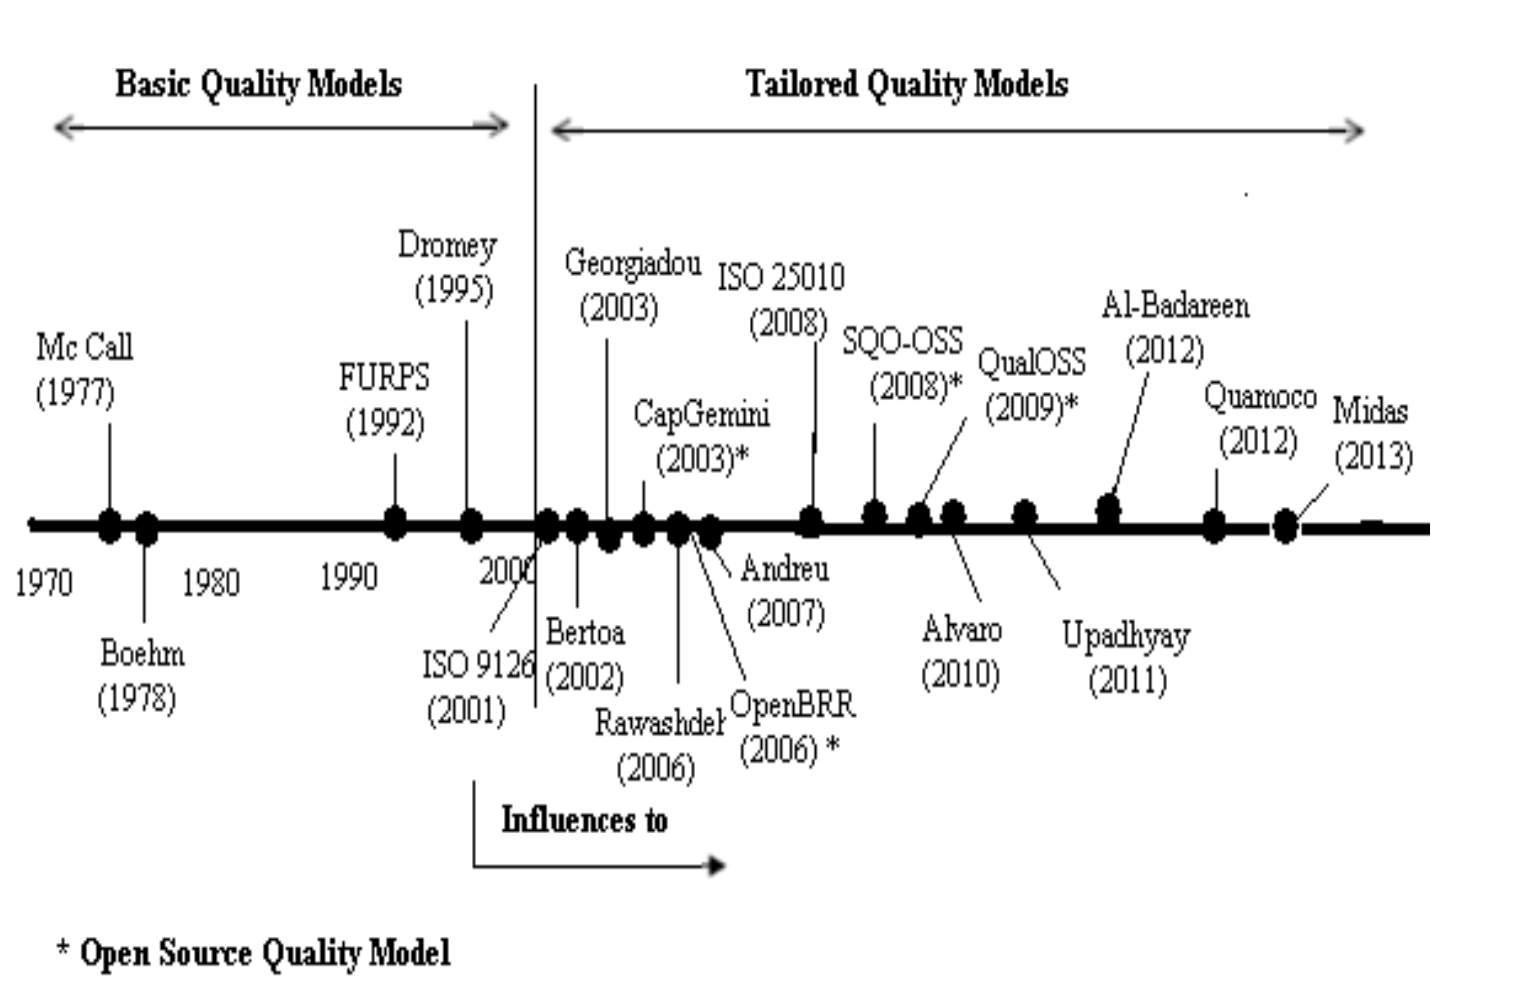
\includegraphics[width=0.8\textwidth]{images/Untitled_12.png}
    \caption{Quality Models. Reproduced from~\cite{quality_models}}
    \label{image_history_of_quality_model}
\end{figure}

ISO/IEC 9126-1 defines the term ``quality model'' as ``the
set of characteristics, and the relationships between them that provides
the basis for specifying quality requirements and
evaluation''~\cite{iso9126} (cited in~\cite{quality_models}). Since different quality models can result in different evaluation
results, the available quality models have to be taken into
consideration before adopting one. \cite{quality_models}
have studied the different quality models (displayed in figure~\ref{image_history_of_quality_model}) and compared
their completeness regarding the characteristics that the models
consider.



To give an overview, a few models are presented along with their
portrayed characteristics in
\cite{quality_models}.
The McCall Model~\cite{mccall}, introduced in 1977, proposes many characteristics to
define software quality, grouped into three higher order groups.
\textbf{Product Review} includes
\textit{Maintenance},
\textit{Flexibility}, and
\textit{Testing}, \textbf{Product Operation}
contains the qualities
\textit{Correct},
\textit{Reliable},
\textit{Efficient},
\textit{Integrity} and
\textit{usability}, and finally \textbf{Product Transition} includes
\textit{Portability},
\textit{Reusability} and
\textit{Interoperability}~\cite{quality_models}. Figure~\ref{image_mccall} shows a representation of the
model.

\begin{figure}[h!]
\centering
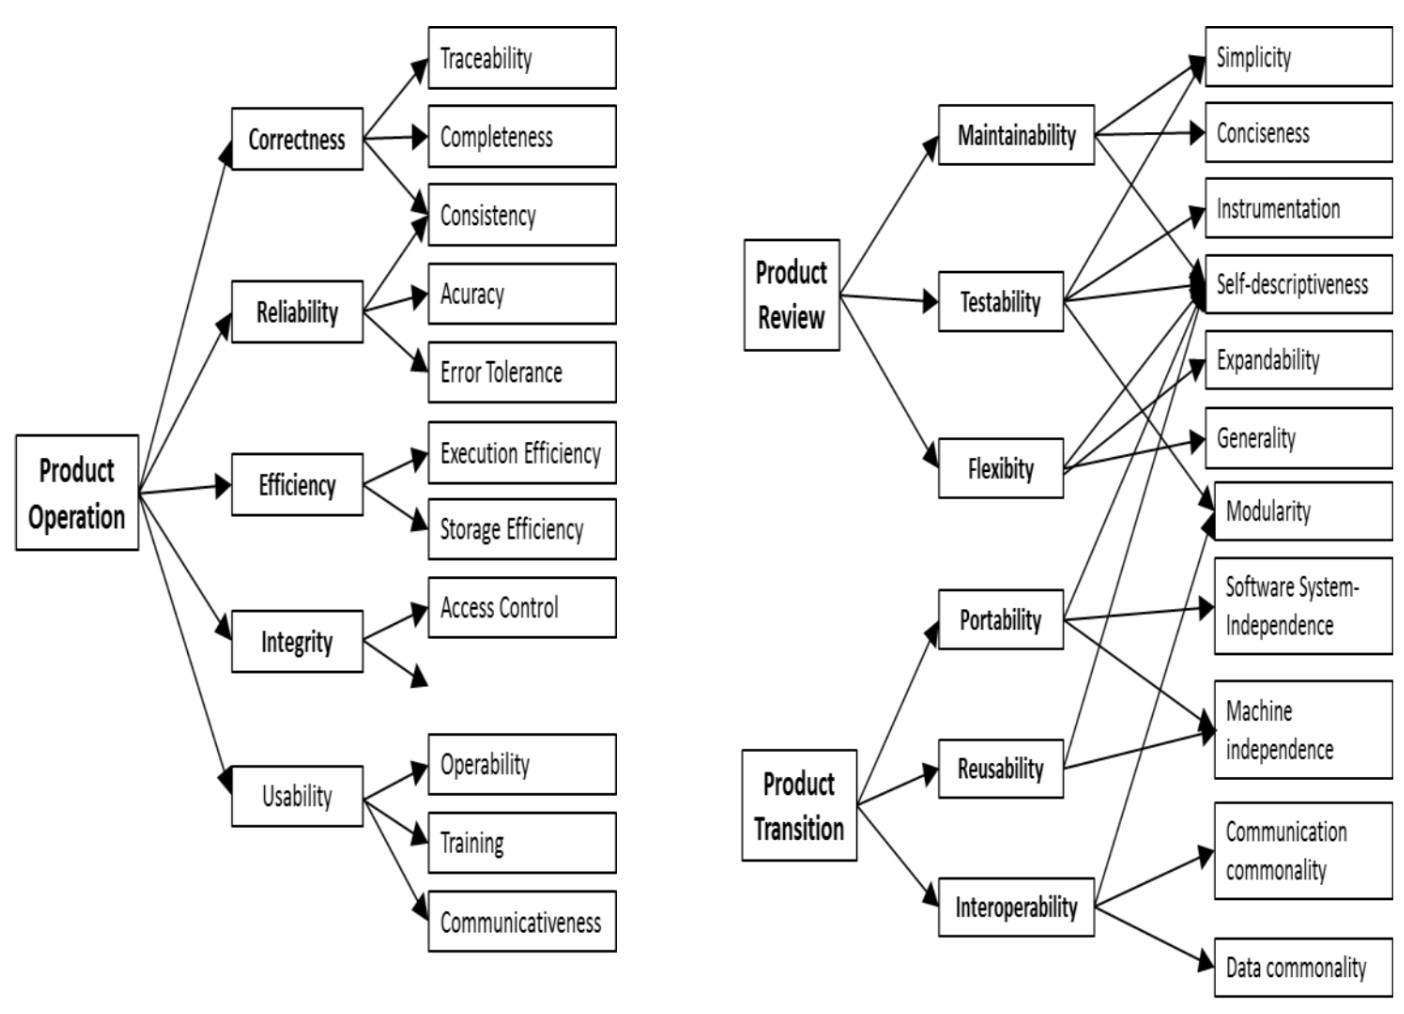
\includegraphics{images/mccall.jpg}
\caption{McCall Quality Model. Reproduced from~\cite{quality_models}}
\label{image_mccall}
\end{figure}

Although the McCall model considers the relation between quality
characteristics and metrics, it lacks in accuracy, since the metrics can
only have a boolean value ~\cite{quality_models}. Moreover, it does not include the
characteristic \textbf{Functionality} or the possibility to add use case
specific characteristics, which can be a drawback for the user~\cite{quality_models}.

The Boehm model~\cite{boehm} presents improvements over the McCall model by adding a
few factors~\cite{quality_models}, as can be seen in figure~\ref{image_boehm}.

\begin{figure}[h!]
\centering
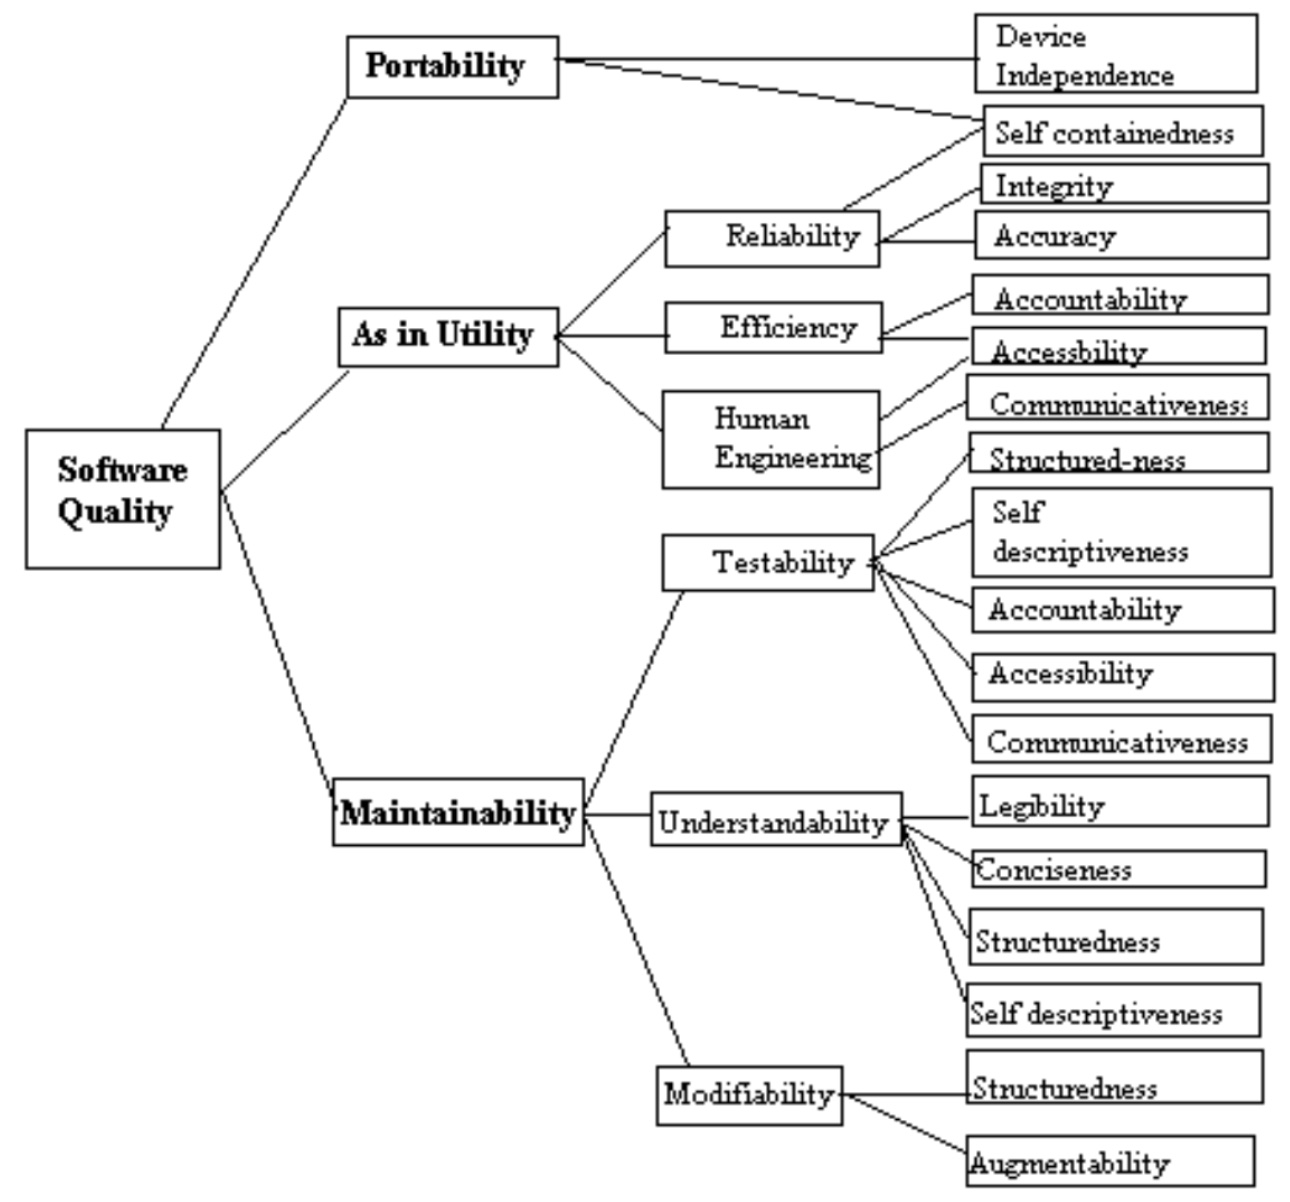
\includegraphics[width=0.7\textwidth]{images/boehm.jpg}
\caption{Boehm Model. Reproduced from~\cite{quality_models}}
    \label{image_boehm}
\end{figure}

The Dromey model~\cite{dromey}, which is depicted in figure~\ref{image_dromey} below,
clusters the characteristics
into four groups: \textit{Correctness}, \textit{Internal}, \textit{Conceptual}, and \textit{Descriptive}~\cite{quality_models}.
Although this model allows for a more dynamic evaluation to be
done, its practical application is unclear. It is therefore used as the
basis for other models~\cite{quality_models}.

\begin{figure}[h!]
\centering
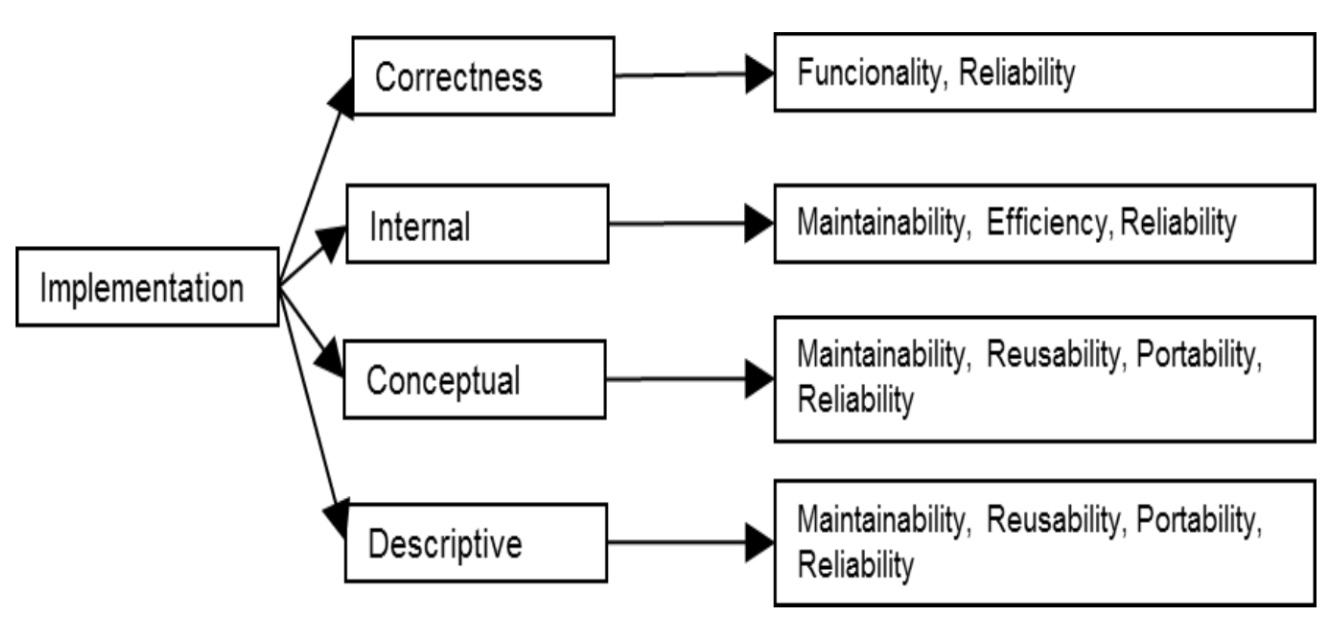
\includegraphics[width=0.7\textwidth]{images/dromey.jpg}
\caption{Dromey Model. Reproduced from~\cite{quality_models}}
    \label{image_dromey}
\end{figure}

%\newpage
The FURPS model established in 1992, is a composition of the
characteristics \textbf{F}unctionality, \textbf{U}sability,
\textbf{R}eliability, \textbf{P}erformance and \textbf{S}upportability
(or Product Support)~\cite{furps},
as displayed in figure~\ref{image_furps}. Although the model differentiates between
functional and non functional requirements, it is missing a few main
characteristics, such as portability~\cite{quality_models}.

\begin{figure}[h!]
\centering
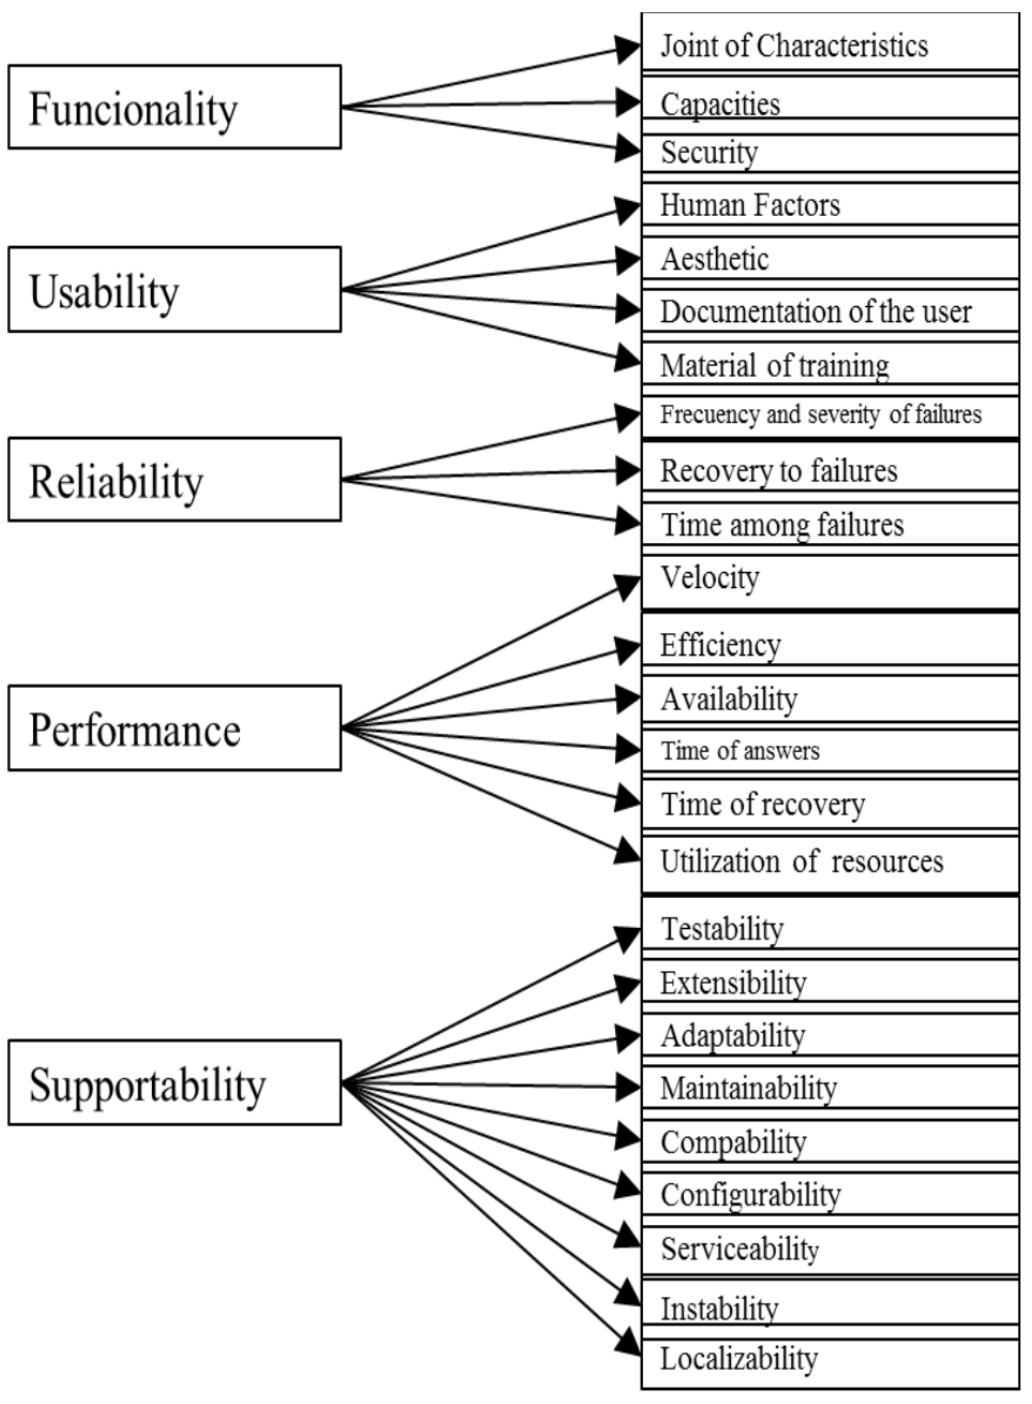
\includegraphics[width=0.5\textwidth]{images/furps.jpg}
\caption{FURPS Model. Reproduced from~\cite{quality_models}}
\label{image_furps}
\end{figure}

The ISO/IEC 9126 model bases on the McCall and Boehm models and
differentiates between external and internal qualities~\cite{dap_model}. Internal quality
attributes, which can be considered as a form of intrinsic quality attributes,
can be evaluated without the
need of executing the software. In contrast, the external quality
attributes can be assessed during the execution~\cite{dap_model}. The model introduces
another group of qualities, Quality in use, which includes the
\textit{effectiveness of the product}, \textit{productivity}, \textit{security offered to the
applications}, and \textit{satisfaction of users}.

\begin{figure}[h!]
\centering
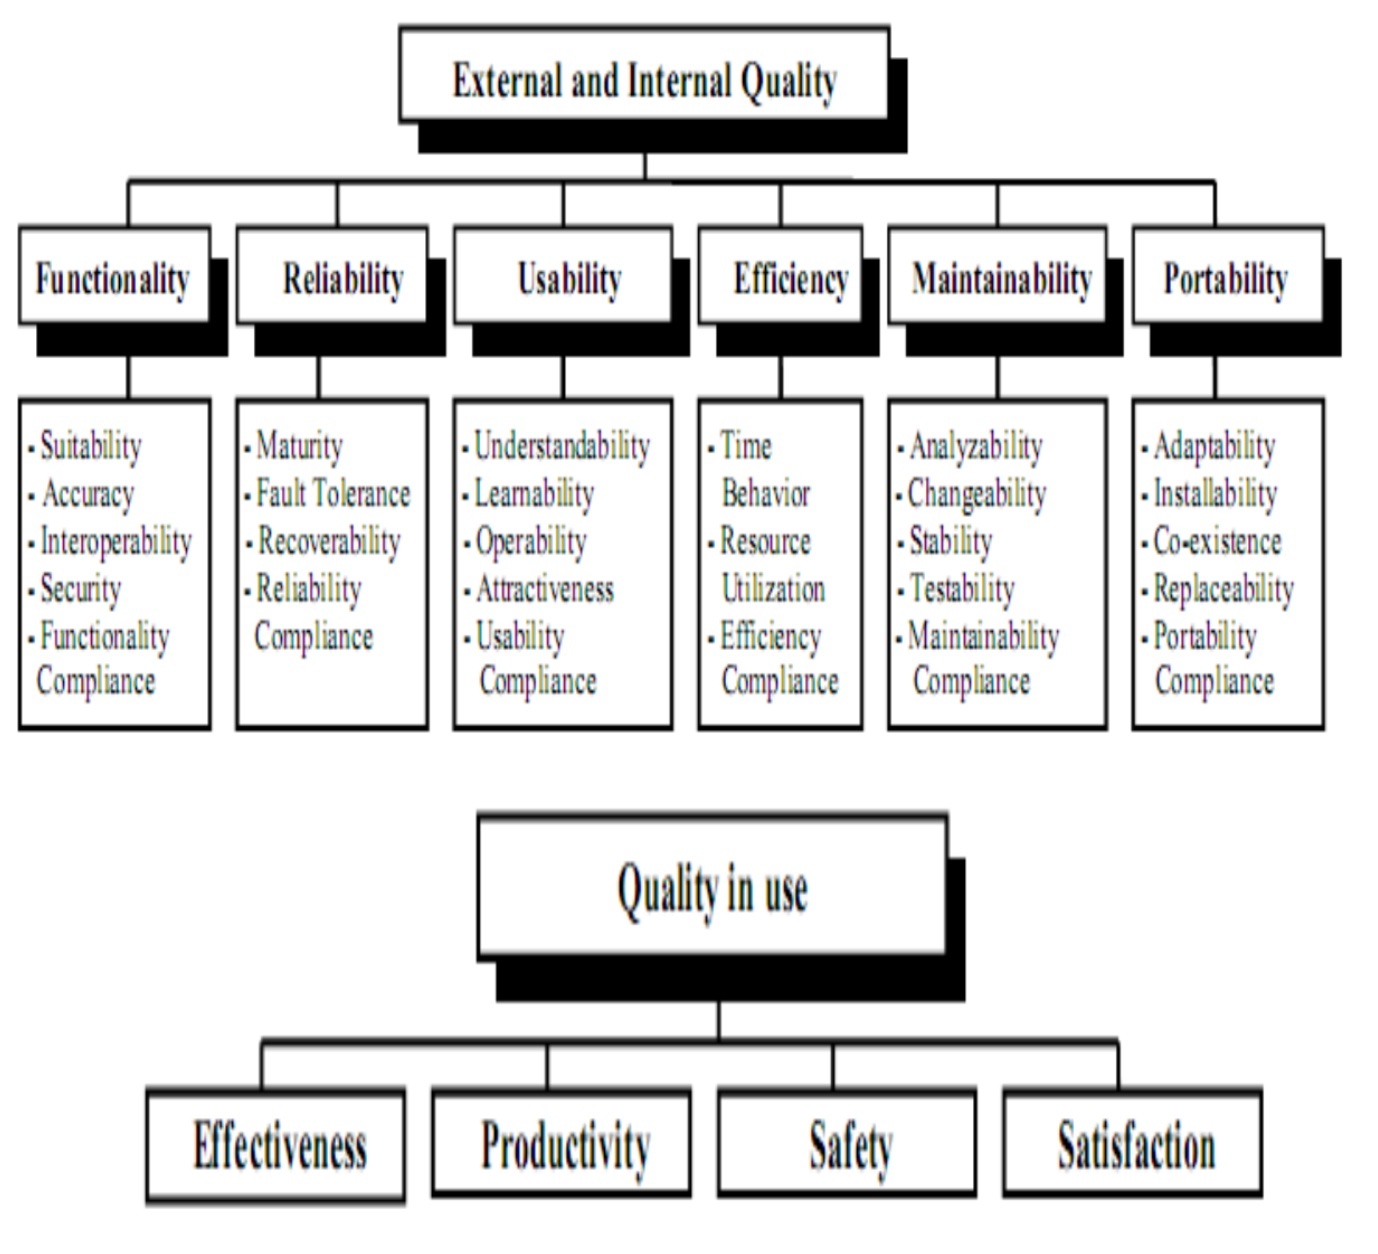
\includegraphics[width=0.7\textwidth]{images/iso-9126.jpg}
\caption{ISO/IEC 9126 Quality Model. Reproduced from~\cite{quality_models}}
\end{figure}

Lastly, the ISO/IEC 25010 Model is an extension of the ISO/IEC 9126~\cite{iso_25010_pdf}. The main improvement lies in the addition of the
characteristics \textbf{Security} and \textbf{Compatibility}~\cite{sqm_comparison}.

\begin{figure}[h!]
\centering
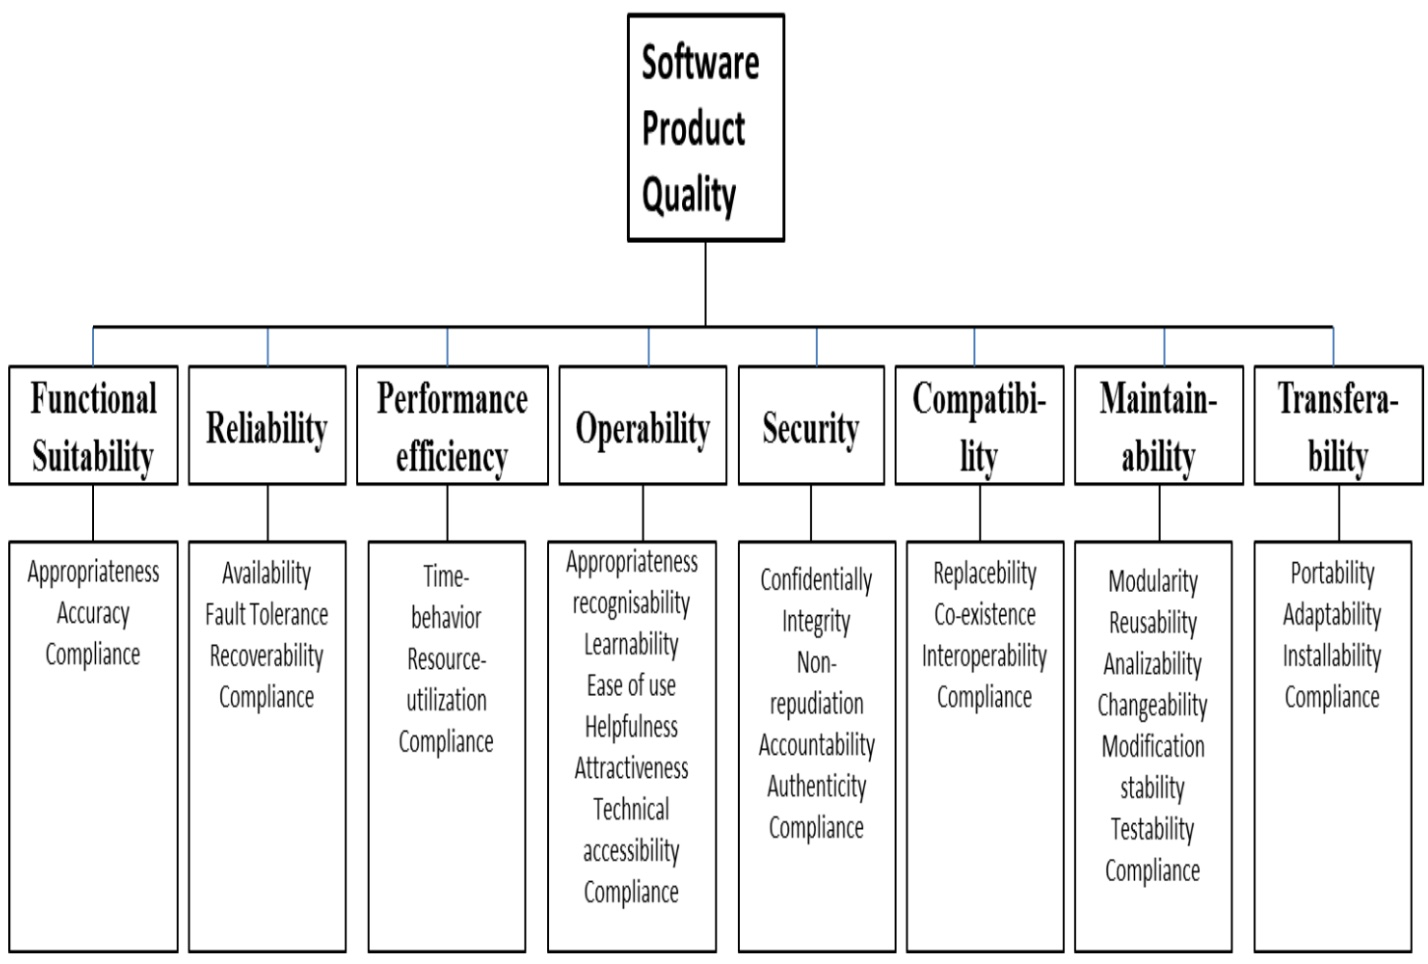
\includegraphics[width=0.7\textwidth]{images/iso-25010.jpg}
\caption{ISO/IEC 25010 Quality Model. Reproduced from~\cite{quality_models}}
\end{figure}

The result of the comparison made by~\cite{quality_models} can be seen in figure~\ref{image_quality_models_comparison},
where ISO/IEC 25010 is regarded as most complete.

\begin{figure}[h!]
\centering
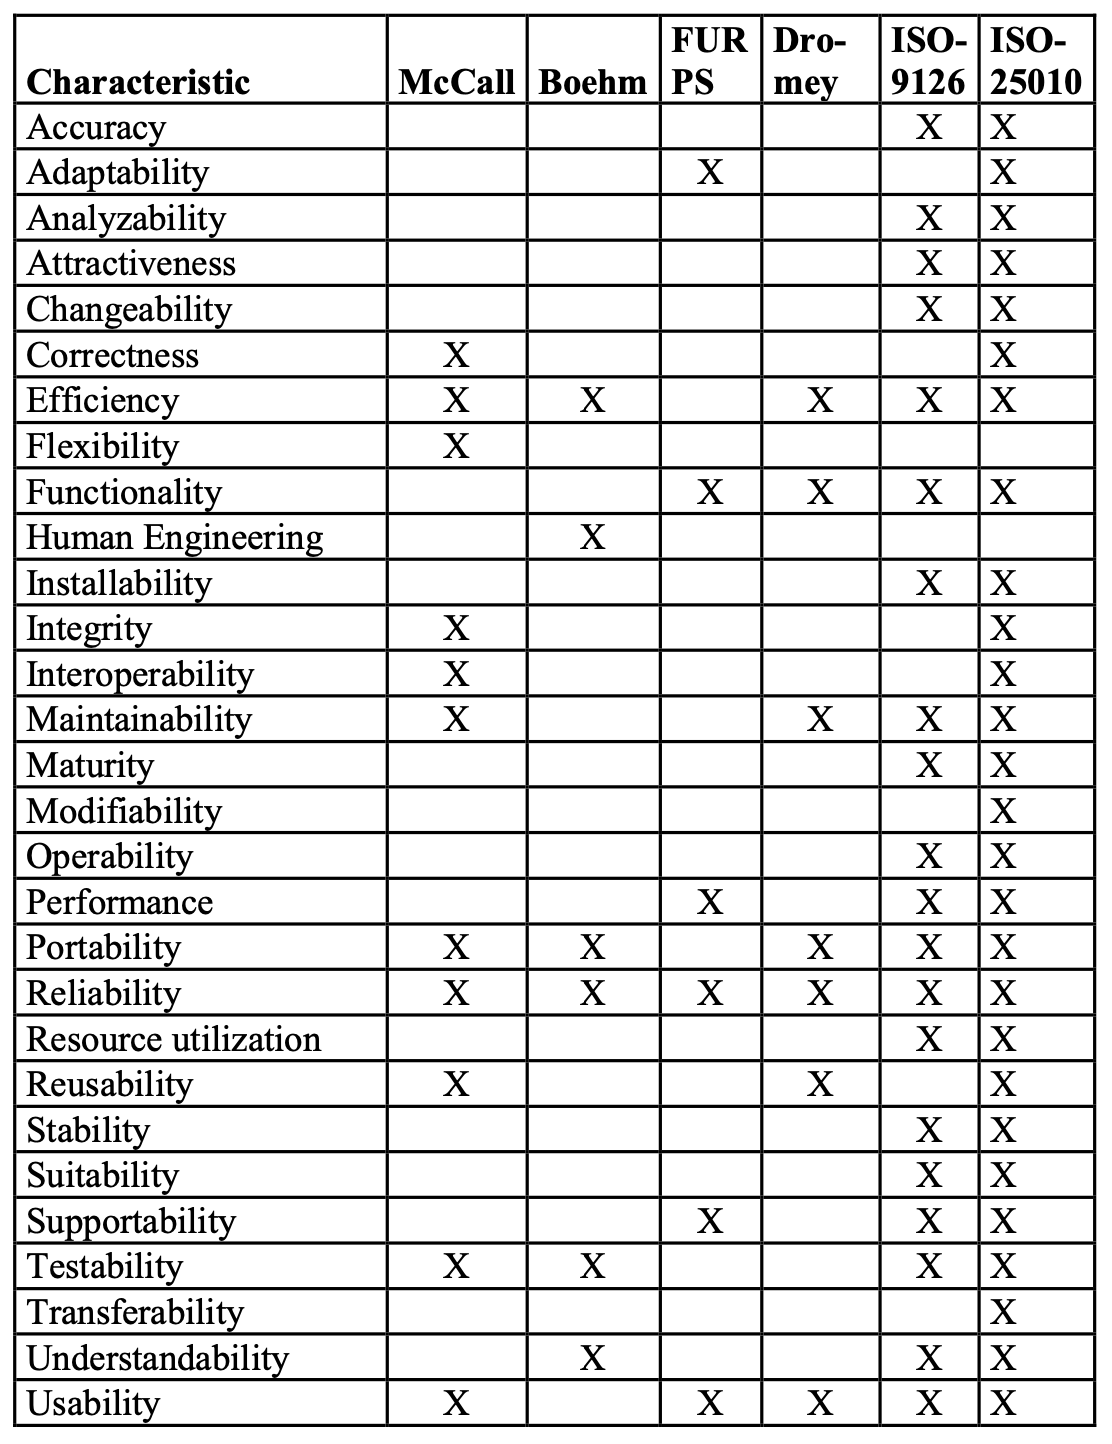
\includegraphics[width=0.8\textwidth]{images/Untitled_13.png}
\caption{Comparision of quality models. Reproduced from~\cite{quality_models}}
    \label{image_quality_models_comparison}
\end{figure}

\clearpage
\hypertarget{the-isoiec-25010-model}{%
\section{ISO/IEC 25010
Model}\label{the-isoiec-25010-model}}

ISO/IEC\ 25010 is a quality model that defines which "quality
characteristics will be taken into account when evaluating the
properties of a software product"~\cite{iso_25010_online}.
This model is used in different areas of software engineering and
architecture, for example in the architecture documentation template
arc42~\cite{arc42_iso}. The quality of a system or software product is thereby
defined as the degree to which it satisfies the needs of the
stakeholders, that according to~\cite{iso_25010_online} are grouped in eight
characteristics: \textbf{Functional Suitability},
\textbf{Performance Efficiency}, \textbf{Compatibility},
\textbf{Usability}, \textbf{Reliability},
\textbf{Security}, \textbf{Maintainability}, and
\textbf{Portability} as portrayed in figure~\ref{image_iso_25010_characteristics}.
Requirements are defined across these characteristics to clarify the
expectations that need to be fulfilled by the presented software
product~\cite{iso_25010_online}.

\begin{figure}
\centering
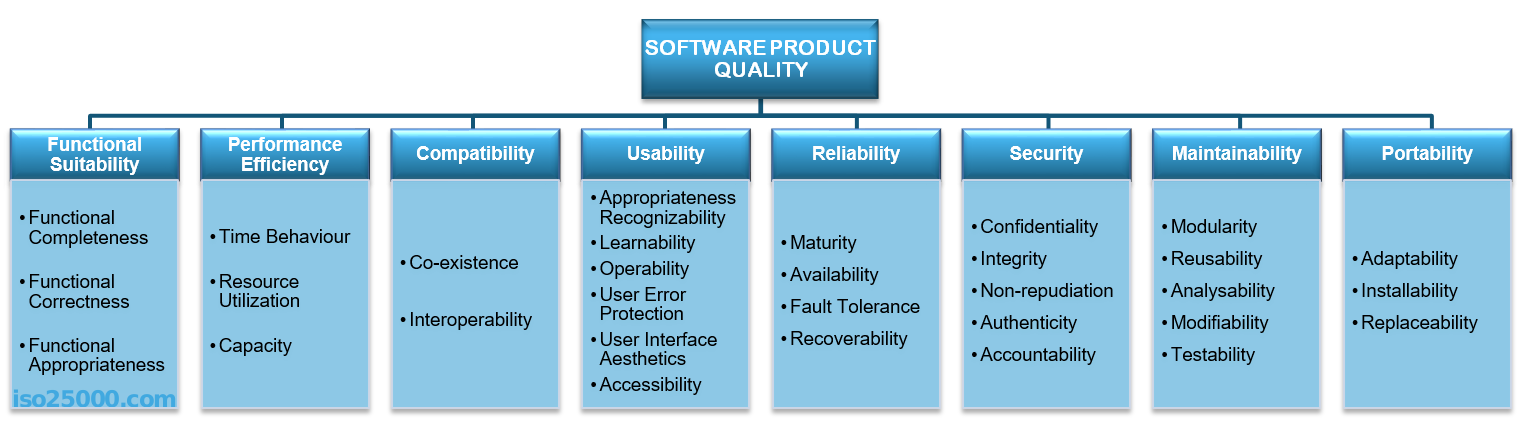
\includegraphics{images/Untitled_14.png}
\caption{Quality characteristics of ISO/IEC 25010 model. Reproduced from~\cite{iso_25010_online}}
    \label{image_iso_25010_characteristics}
\end{figure}

\textbf{Functional Suitability} is the first characteristic of ISO/IEC 25010 and is defined
as the ``degree to which a product or system provides functions that
meet stated and implied needs when used under specified conditions''\cite{iso_25010_online}.
This includes prominently \textit{Functional Completeness}, which refers to the
extend to which the tasks/objectives of the user are covered, \textit{Functional
Correctness}, meaning to which degree the system provides the ``correct
results with the needed degree of precision''\cite{iso_25010_online} and \textit{Functional appropriateness},
and how easy the tasks and objectives are accomplished~\cite{iso_25010_online}.

The second characteristic is \textbf{Performance Efficiency}, which considers
the performance of the software product in regard to its \textit{Time Behavior},
\textit{Resource Utilization}, and \textit{Capacity} (maximum limits)\cite{iso_25010_online}.

The third characteristic is \textbf{Compatibility} and contains two pillars:
\textit{Co-existence}, the extend to which it can function efficiently
``while sharing a common environment or resources with other products''\cite{iso_25010_online_page_2}, and
\textit{Interoperability}, referring to ``the ability of two or more software
components to cooperate despite differences in language, interface, and
execution platform''~\cite{interoperability}.

The fourth characteristic is \textbf{Usability}, which focuses on the interaction
between the user and the software product and includes the
sub-characteristics: \textit{Operability}, \textit{Learnability}, \textit{User Error Protection},
\textit{Appropriateness Recognizability}, \textit{User Interface Aesthetic}, and
\textit{Accessibility}~\cite{iso_25010_online_page_2}.

The fifth characteristic is \textbf{Reliability}, which refers to the degree
to which the software product performs ``specified functions under
specified conditions for a specified period of time''~\cite{iso_25010_online_page_2}.
This characteristic comprises the sub-characteristics
\textit{Maturity} (the degree to which the needs for reliability are
met under normal operation), \textit{Fault Tolerance} (to which extend the
software product works correctly in the presence of software or hardware
faults), and \textit{Recoverability} (to which degree the system can
recover its normal state and affected data after an interruption or a
failure) and \textit{Accessibility}~\cite{iso_25010_online_page_2}.

The sixth characteristic is \textbf{Security} and is defined by the
sub-characteristics \textit{Confidentiality} (the degree to which data
is accessible to only authorized entities), \textit{Integrity} (the
protection of data from unauthorized changes), \textit{Non-repudiation}
(committed actions or events can be proved and cannot be repudiated
afterwards), \textit{Accountability} (where actions can be traced back
to the committing entity), and \textit{Authenticity} (where ``the identity
of a subject or resource can be proved to be the one claimed'')~\cite{iso_25010_online_page_3}.

The next characteristic is \textbf{Maintainability} and includes
different sub-characteristics ranging from \textit{Modularity} (the
degree to which the product is split into components whose changes don't
affect others) to \textit{Reusability}, \textit{Testability},  \textit{Modifiability} (how easy
it is to modify the product without introducing bugs), and
finally \textit{Analyzability} (how easy it is to assess the impact of
changes as well as the ease of diagnosis)~\cite{iso_25010_online_page_3}.

The last characteristic is \textbf{Portability} and refers to the
ability of the product to be transferred to another environment. It
comprises \textit{Adaptability} (the degree to which the product can
evolve or adapt to a changing environment), \textit{Installability} (how
easy it is to be installed or removed from a specified environment), and
\textit{Replaceability} (how easy it is to be replaced by another
product with the same purpose in the same environment)~\cite{iso_25010_online_page_3}.

\clearpage
\hypertarget{dap-model}{%
\section{DAP classification}\label{dap-model}}

When it comes to practically applying the above mentioned ISO/IEC 25010 standard,
many ambiguities arise. Namely, no instructions are provided on how to measure
the defined software criteria. \cite{dap_model}
addresses this problem by highlighting that the umbrella term ``quality
model'' includes models that aim to fulfill different purposes. For
example, the goal of ISO/IEC 9126 (the predecessor of ISO/IEC 25010) is to
\textbf{define} quality, whereas the maintainability index~\cite{maintainability_index}, a
metric-based approach, is used to \textbf{assess} quality, and finally
stochastic models such a reliability growth models (RGMs) \cite{rgm} can be
used to \textbf{predict} quality~\cite{dap_model}. Although the specified goals are
different, these models depend on each other. Quality can't be assessed without
first being defined. Similarly, it is inconceivable to predict quality
without knowing how to measure it \cite{dap_model}.
Figure~\ref{image_dap} illustrates the relation
between the three model categories: Definition, Assessment and
Prediction (DAP), as well as the positioning of ISO/IEC 9126, MI and RGM,
and an ideal model which covers all three aspects.

\begin{figure}
\centering
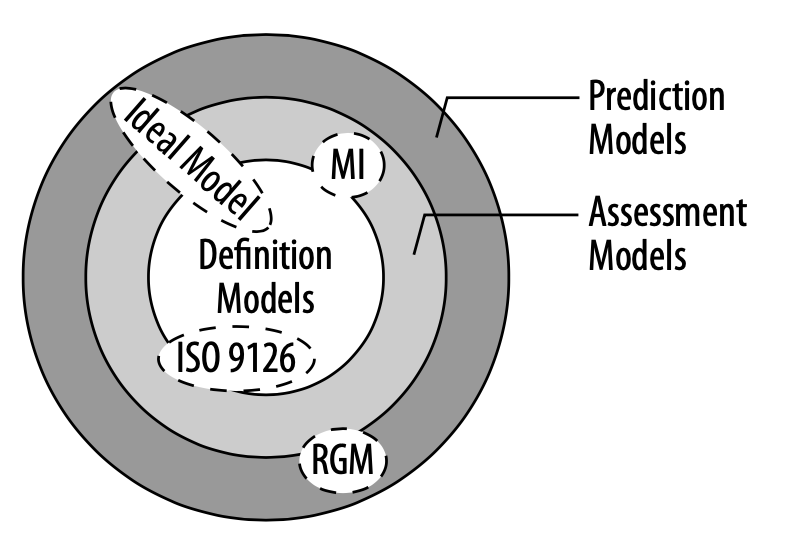
\includegraphics[width=0.6\textwidth]{images/Untitled_15.png}
\caption{DAP classification for Quality Models: Reproduced from~\cite{dap_model}}
    \label{image_dap}
\end{figure}

Another critique on the existing quality models is the lack of precision
that leads to different possible interpretations~\cite{dap_model}. Since software
systems can vary largely, the quality models should offer additionally
the possibility of customization~\cite{dap_model}.

In~\cite{sqm_comparison},
a comparison of Open Source Software (OSS) Quality Models, that are
based on ISO/IEC 25010 and ISO/IEC 9126, was conducted. The compared OSS Quality
Models include \emph{Open Source Maturity Model (OSMM)}~\cite{osmm}, \emph{QSOS}~\cite{qsos}, \emph{Open Business Readiness Rating (Open BRR)} \cite{openbrr}, \emph{Sung et
al.~Model}~\cite{sung_model}, \emph{QualOSS}~\cite{qualoss}, \emph{OMM} \cite{omm}, \emph{SQO-OSS}~\cite{sqo_oss_1,sqo_oss_2} and \emph{Evaluation Framework for Free/Open souRce projecTs
(EFFORT)}~\cite{effort}.

The study~\cite{sqm_comparison} resulted in EFFORT being favored over the rest. One of the
reasons is that EFFORT is a second generation~\cite{difference_between_2_generation} Free/Libre and Open Source
Software (FLOSS) quality model. It was preferred above QualOSS since it included
characteristics from both Product Quality and Quality in Use ~\cite{sqm_comparison}.
Additionally, there have been practical applications of the model within
the context of Customer Relationship Management (CRM)
~\cite{effort_crm} and Enterprise Resource Planning (ERP) Systems
~\cite{effort}. Another reason for selecting EFFORT, is that it comes
close to the ideal model proposed in the DAP model: The definition
aspect is provided by specifying the quality characteristics in form of
goals and questions, the assessment aspect through the usage of metrics,
and the prediction aspect through the consideration of community
trustworthiness and product attractiveness, as is presented in further
detail in the next chapter.

\clearpage
\hypertarget{effort}{%
\chapter{EFFORT}\label{effort}}

EFFORT, short for \textbf{E}valuation \textbf{F}ramework for
\textbf{F}ree/\textbf{O}pen sou\textbf{R}ce projec\textbf{T}s, is
a framework which supports not only the evaluation of product quality but also
community trustworthiness and product attractiveness~\cite{effort}. Additionally
the framework is defined in a generic manner and can be instantiated to
analyze software systems and products within a specific context.

\hypertarget{the-effort-baseline-version}{%
\section{EFFORT Baseline
Version}\label{the-effort-baseline-version}}

As an Open Source Software Quality Model, EFFORT leverages the
advantages of OSS for generating extensive results.

\begin{figure}[h!]
    \centering
    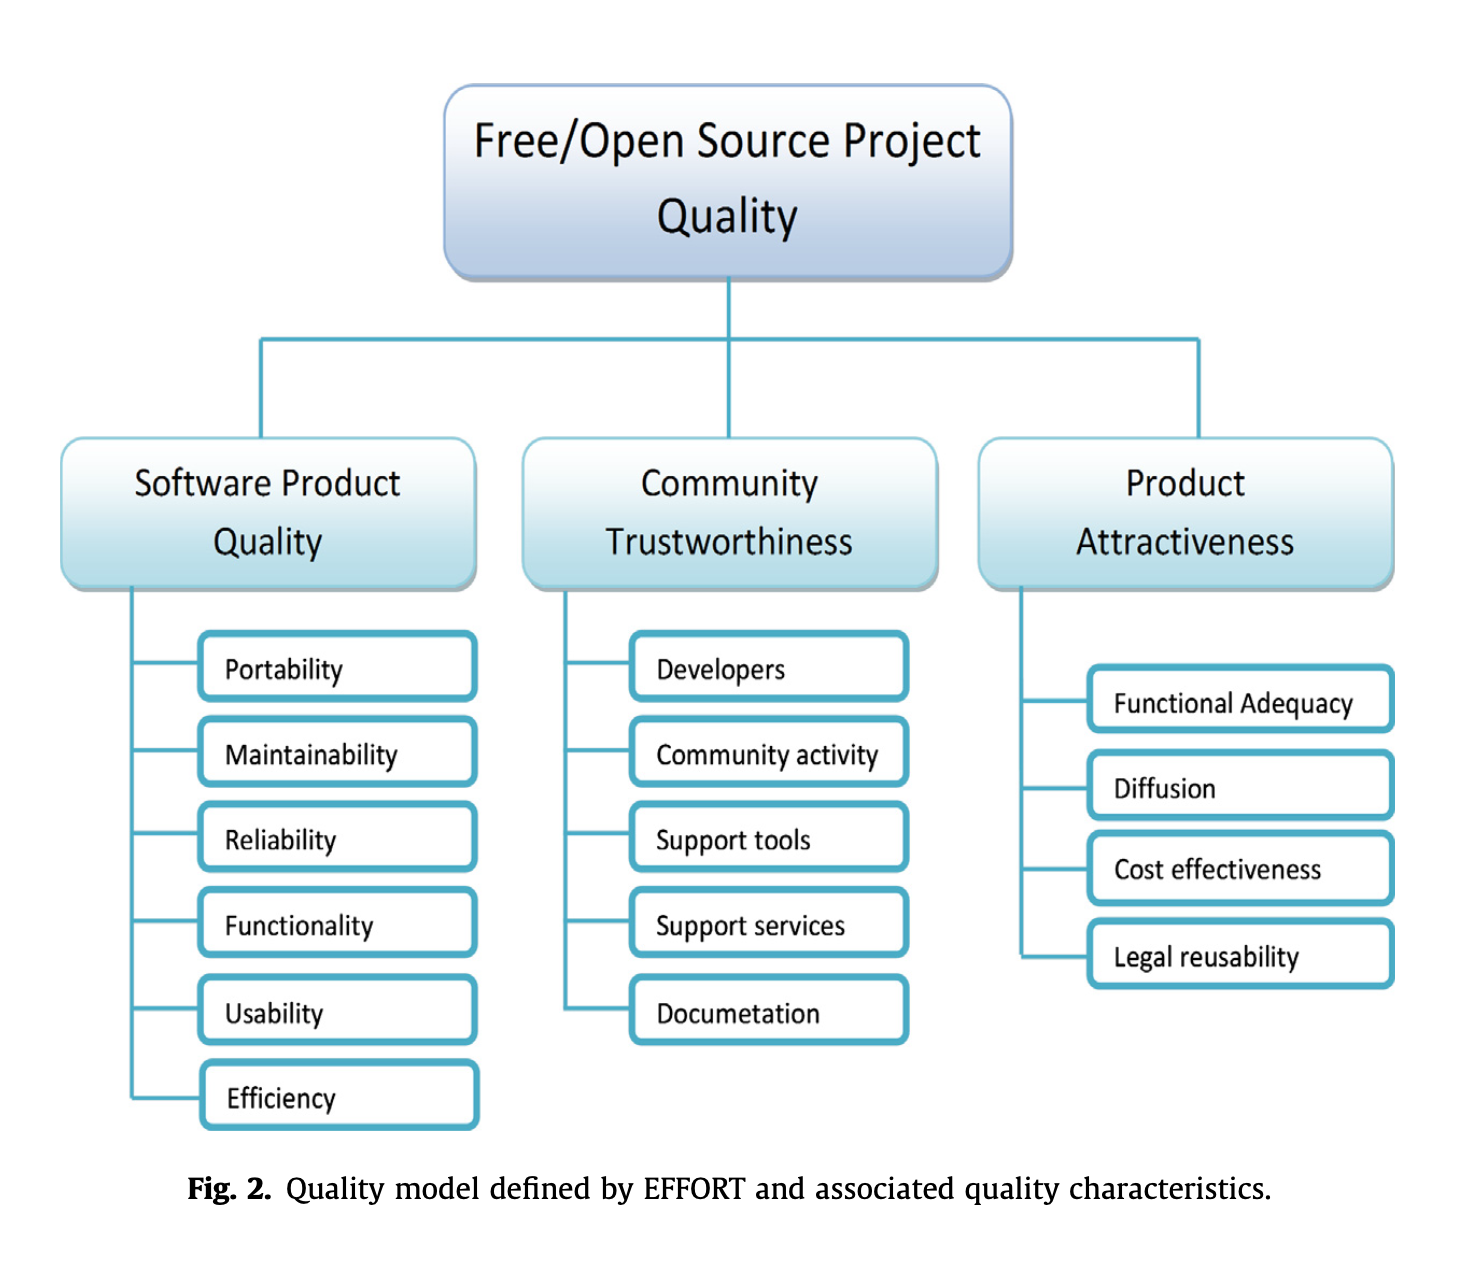
\includegraphics[width=0.6\textwidth]{images/Untitled_18.png}
    \caption{Quality model defined by EFFORT and associated quality characteristics. Reproduced from ~\cite{effort}}
    \label{image_effort_characteristic}.
\end{figure}

The quality of a
software product according to EFFORT is a combination of three main
quality characteristics~\cite{effort}, as shown in Figure~\ref{image_effort_characteristic}.

\begin{itemize}
\tightlist
\item
  \textbf{Quality of the product}, which is evaluated on the basis of
  the ISO/IEC 9126 standard.
\item
  \textbf{Trustworthiness of the community} of developers and
  contributors, which is an indicator of ``the degree of trust that a
  user has in a community with respect to the
  support offered''~\cite{effort}
\item
  \textbf{Product attractiveness}, which ``considers all the factors that
  influence the adoption of a product by a potential user, who perceives
  convenience and usefulness in using it''~\cite{effort}.
\end{itemize}


In order to specify the proposed characteristics and
sub-characteristics, the Goal/Question/Metric (GQM) paradigm~\cite{gqm} is used.
The Goal/Question/Metric paradigm is ``a mechanism for defining
and interpreting software measurement'' that ``represents a systematic approach for
tailoring and integrating goals with models of the software processes,
products and quality perspectives of interest based upon the specific
needs of the project and the organization''~\cite{gqm}.

A critique made by~\cite{dap_model} is that most definition models
structure their quality attributes in a
hierarchy, which causes difficulty while locating elements and can lead
to redundancies~\cite{dap_model}. Luckily, this issue is addressed in the GQM
paradigm where questions can contribute to more than one goal \cite{gqm}. This can
be seen in figure~\ref{image_qgm_tree}, in which the goals
\emph{Goal2} and \emph{Goaln} contribute to the same question
\emph{Question6}.

\begin{figure}[h!]
\centering
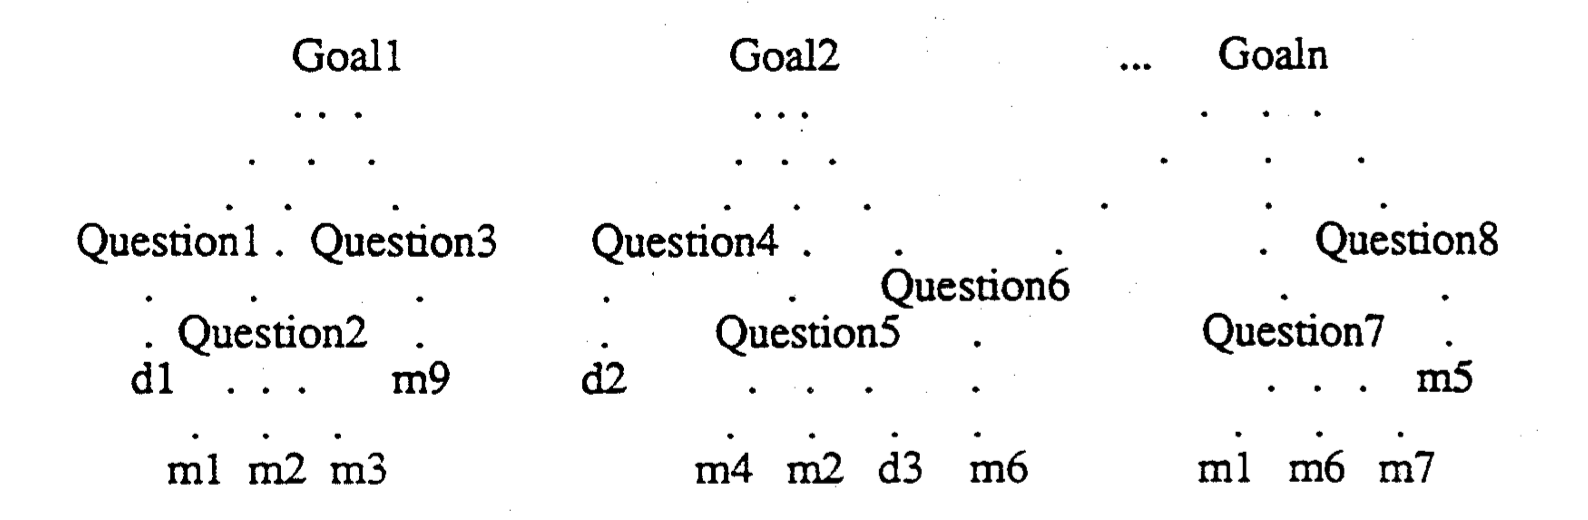
\includegraphics[width=0.7\textwidth]{images/Untitled_19.png}
    \caption{The structure of Goals, Questions and Metrics in the GQM Paradigm~\cite{gqm}}
    \label{image_qgm_tree}
\end{figure}

Within GQM, the goals need to be specified, which are refined into a set of quantifiable
questions that, in turn, define the metrics used to measure the corresponding
outcomes~\cite{gqm}. Because of the large scope of the first goal of
EFFORT, \textit{Software Product Quality}, its subcategories are modeled as
sub-goals. Figures~\ref{image_effort_table_3},~\ref{image_effort_table_4},~\ref{image_effort_table_5},~\ref{image_effort_table_6},
and~\ref{image_effort_table_7} show the questions related to each goal
along with their associated metrics.

\begin{figure}[h!]
\centering
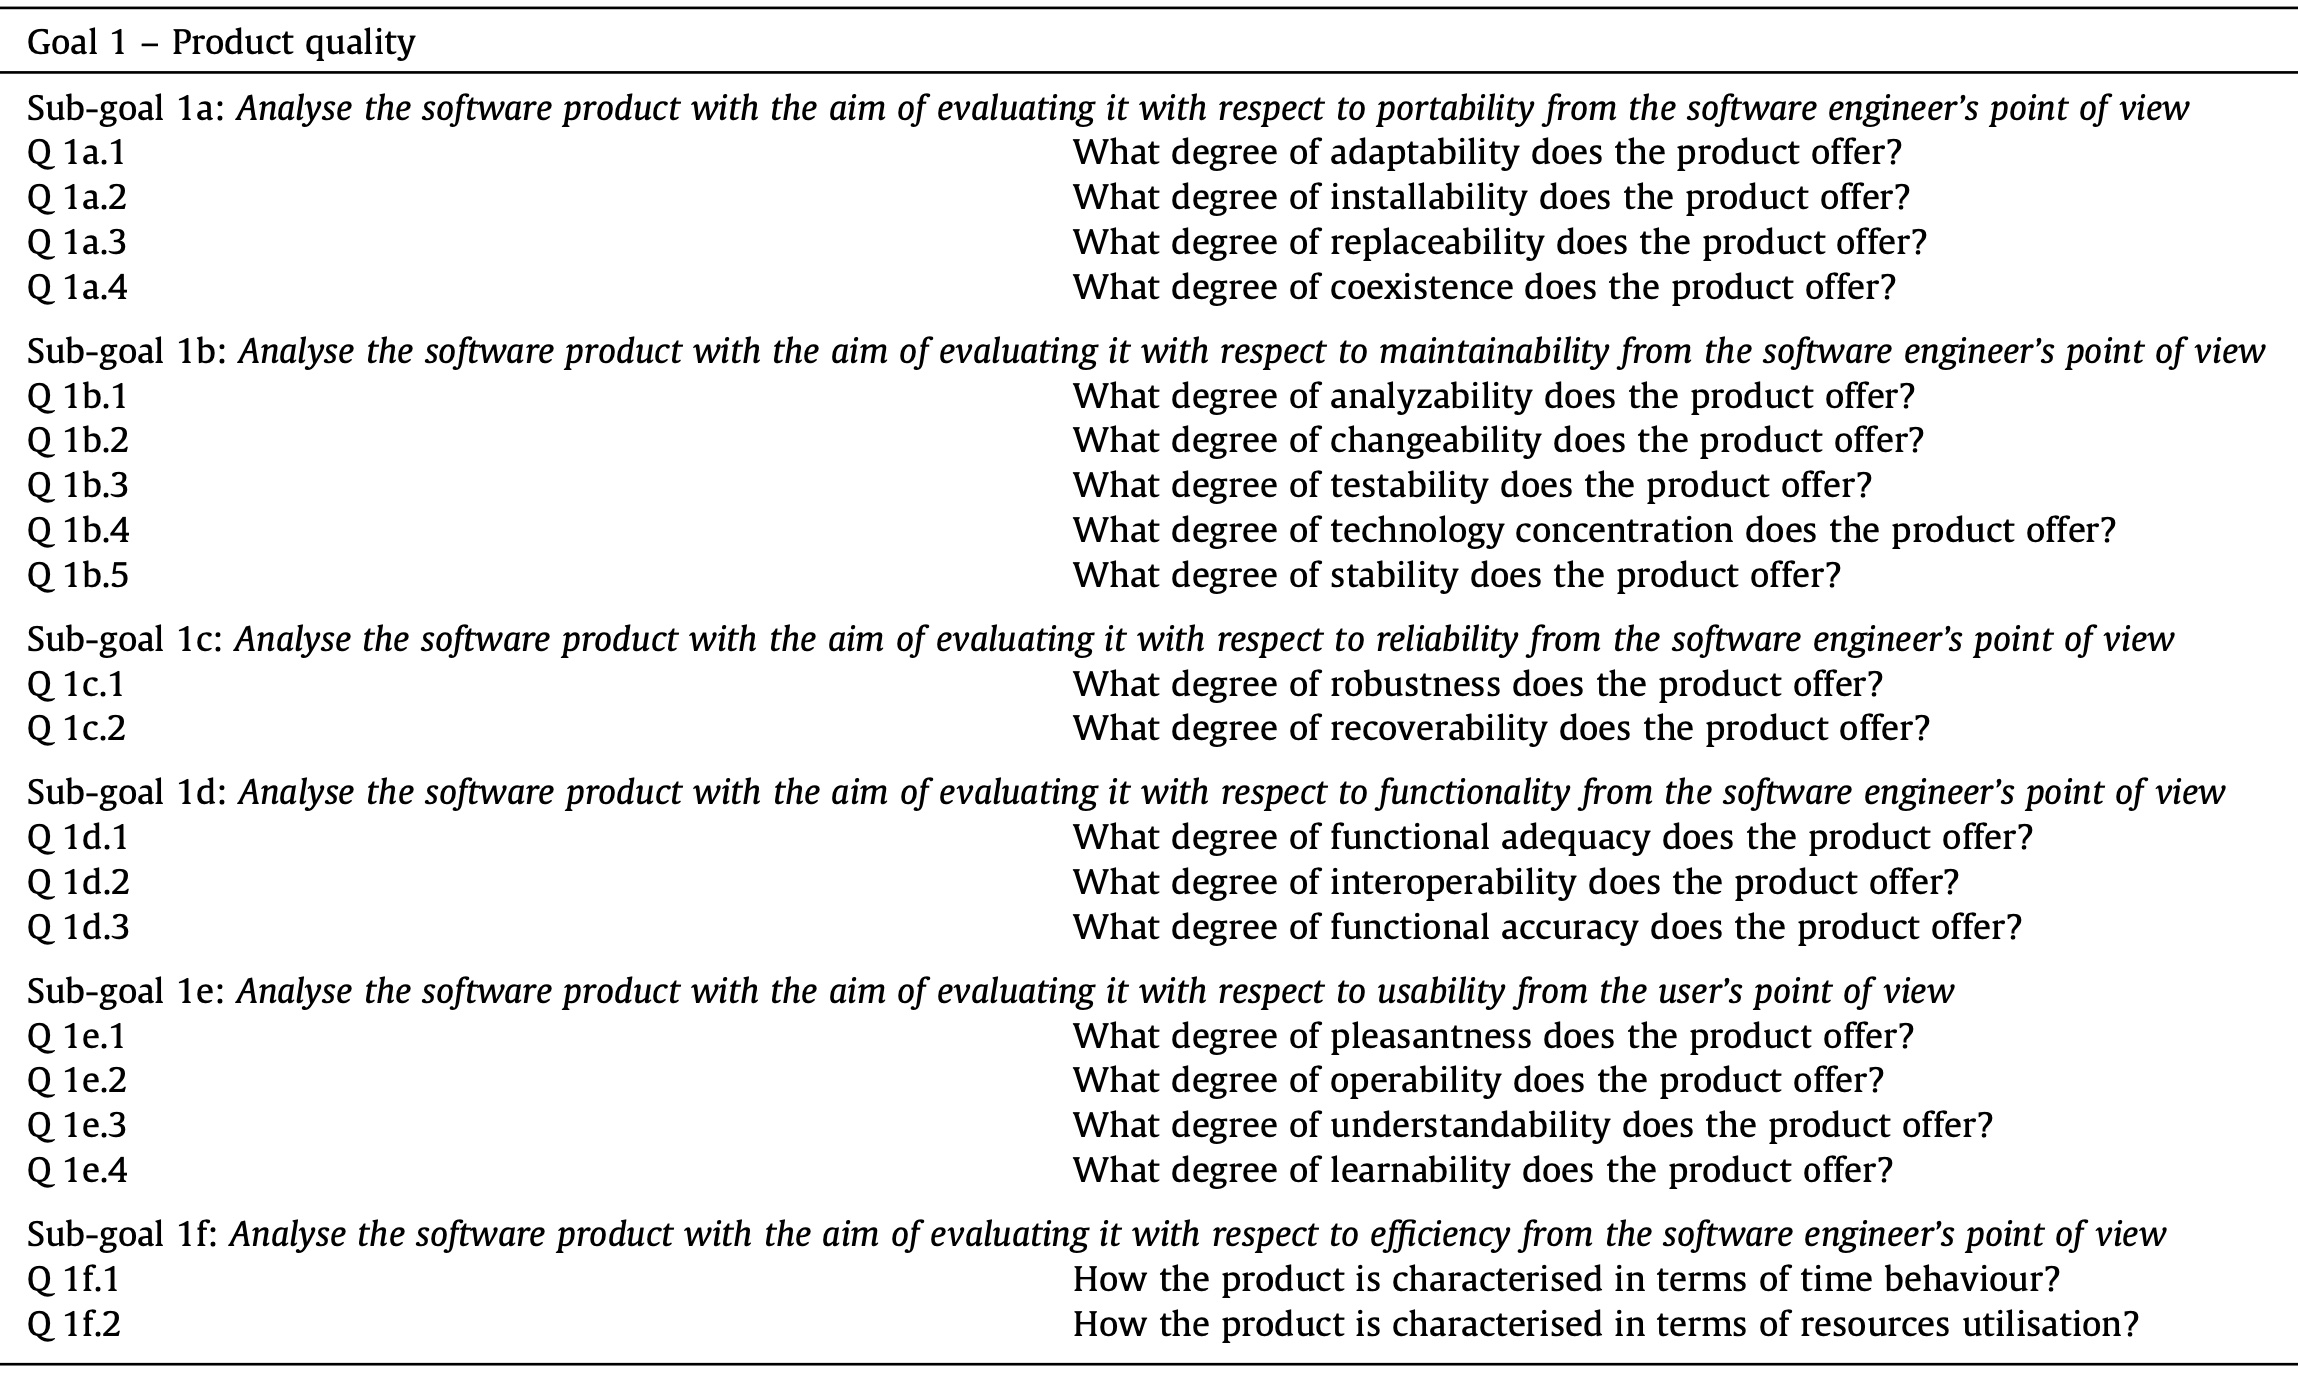
\includegraphics{images/table_3}
\caption{Questions in the EFFORT measurement framework pertaining to product quality. Reproduced from~\cite{effort}}
    \label{image_effort_table_3}
\end{figure}

\begin{figure}[h!]
\centering
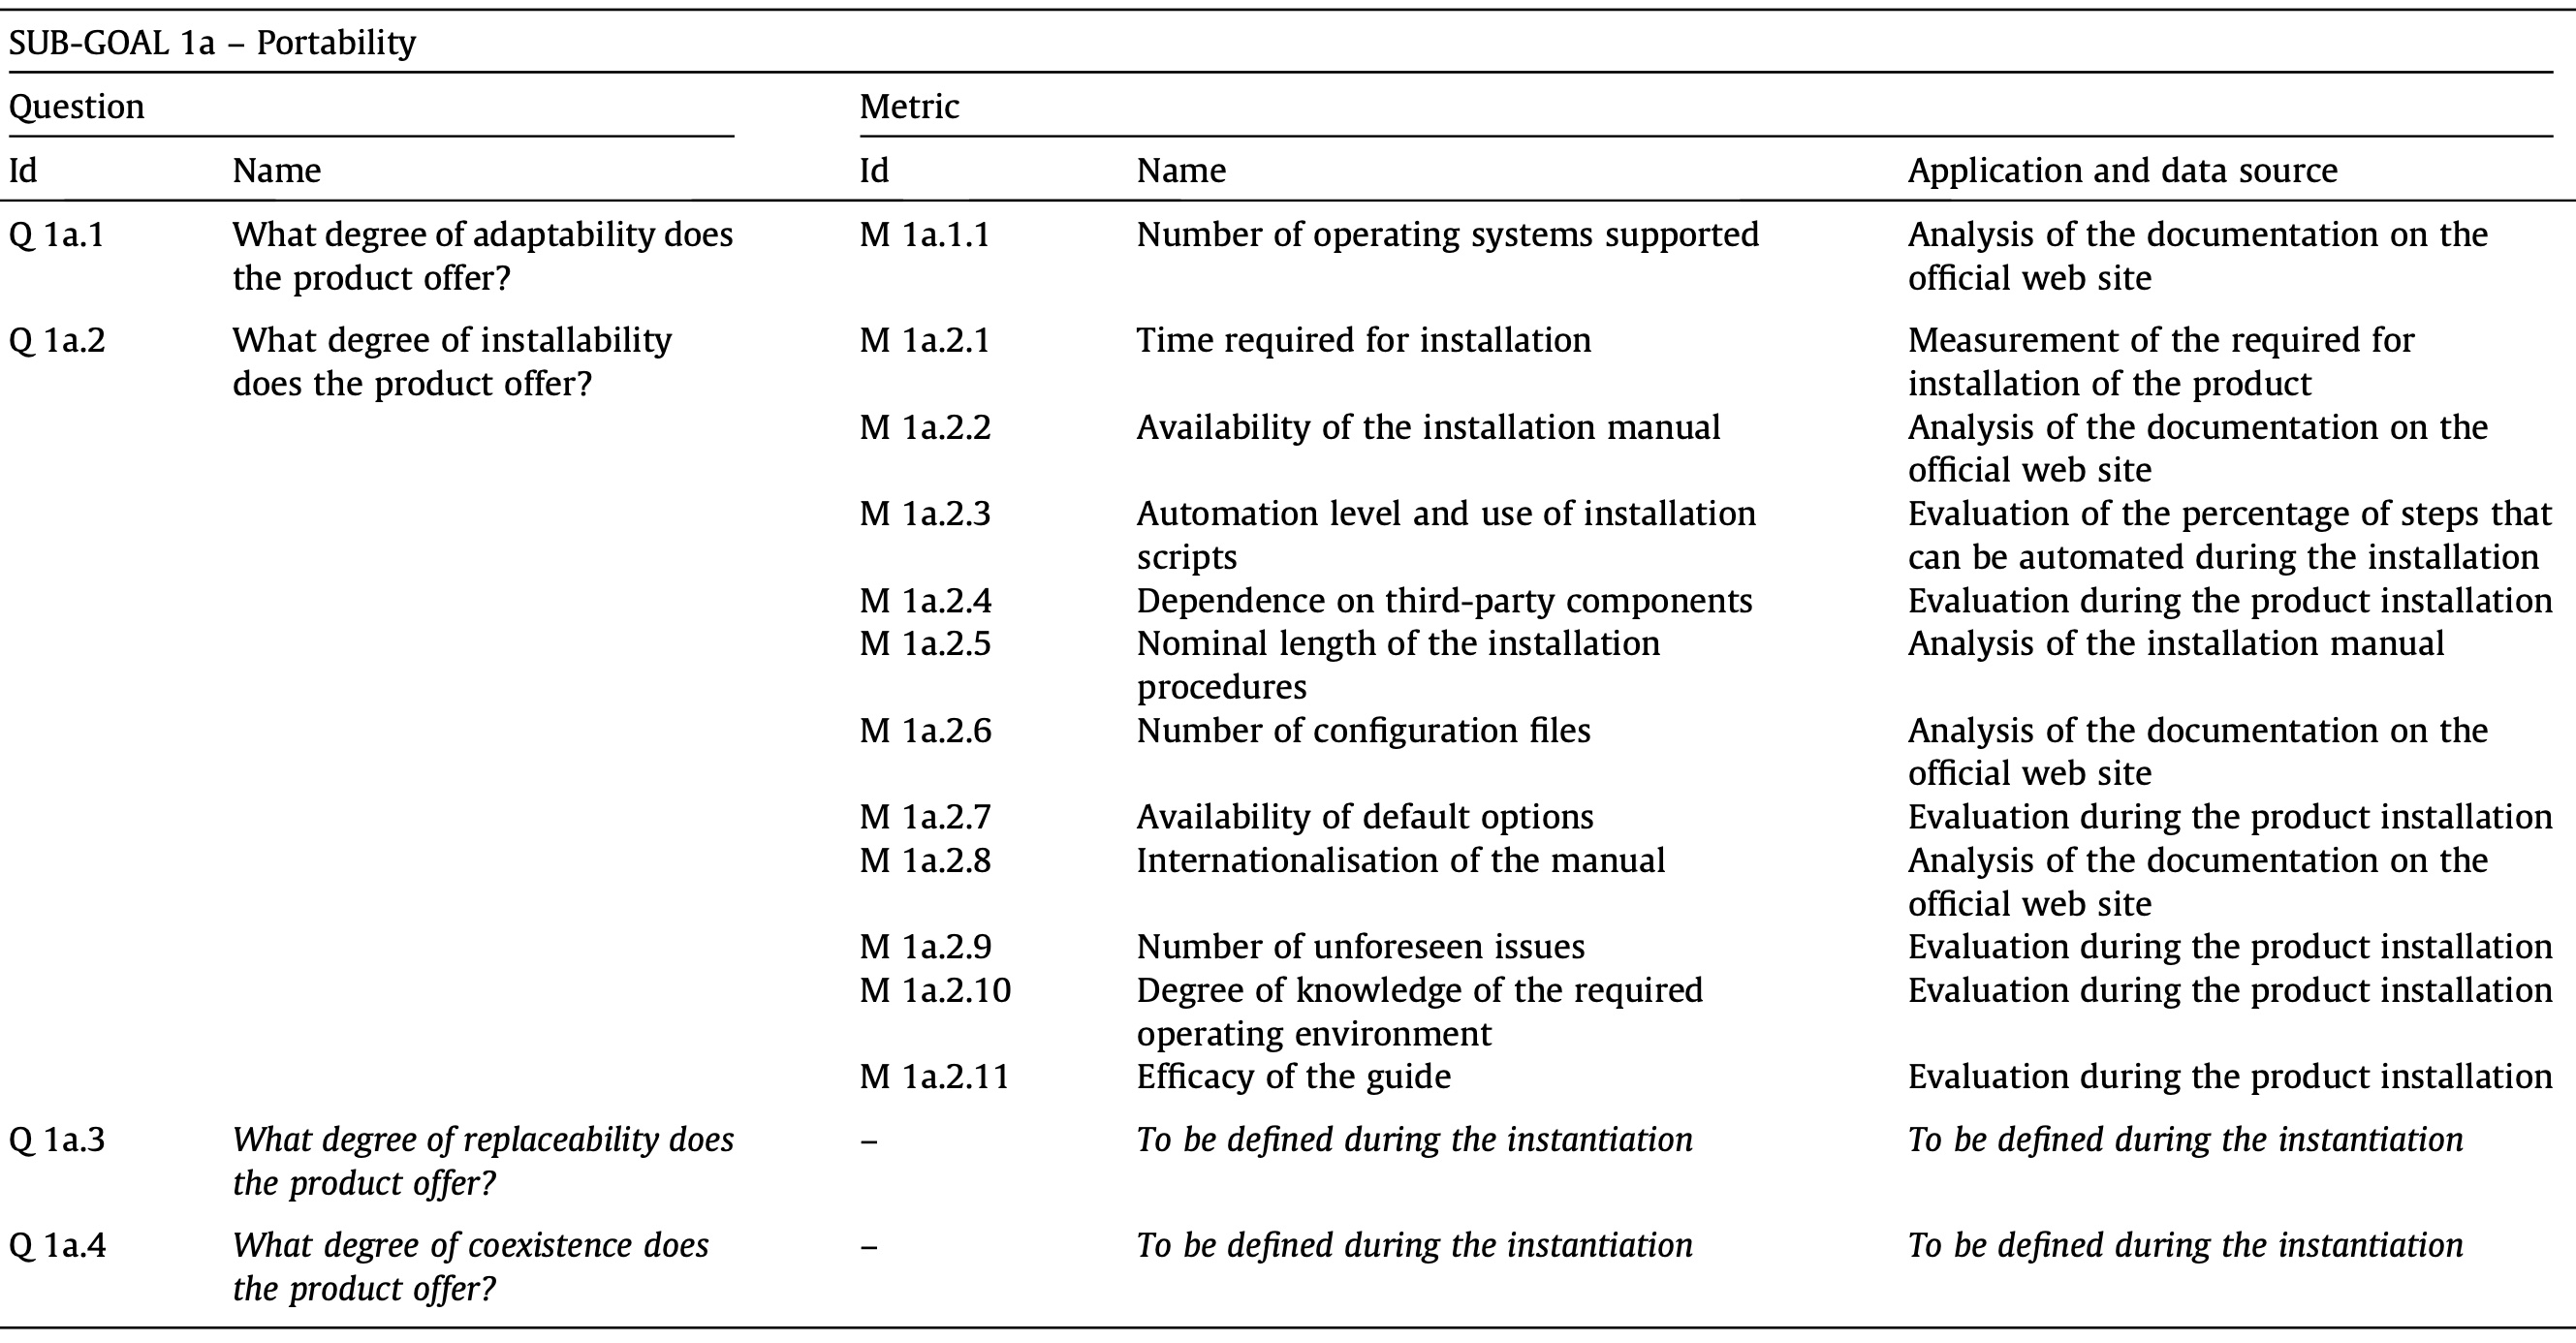
\includegraphics{images/table_4}
\caption{Questions and metrics in the EFFORT measurement framework pertaining to sub-goal 1a. Reproduced from~\cite{effort}}
\label{image_effort_table_4}

\end{figure}

\begin{figure}[h!]
\centering
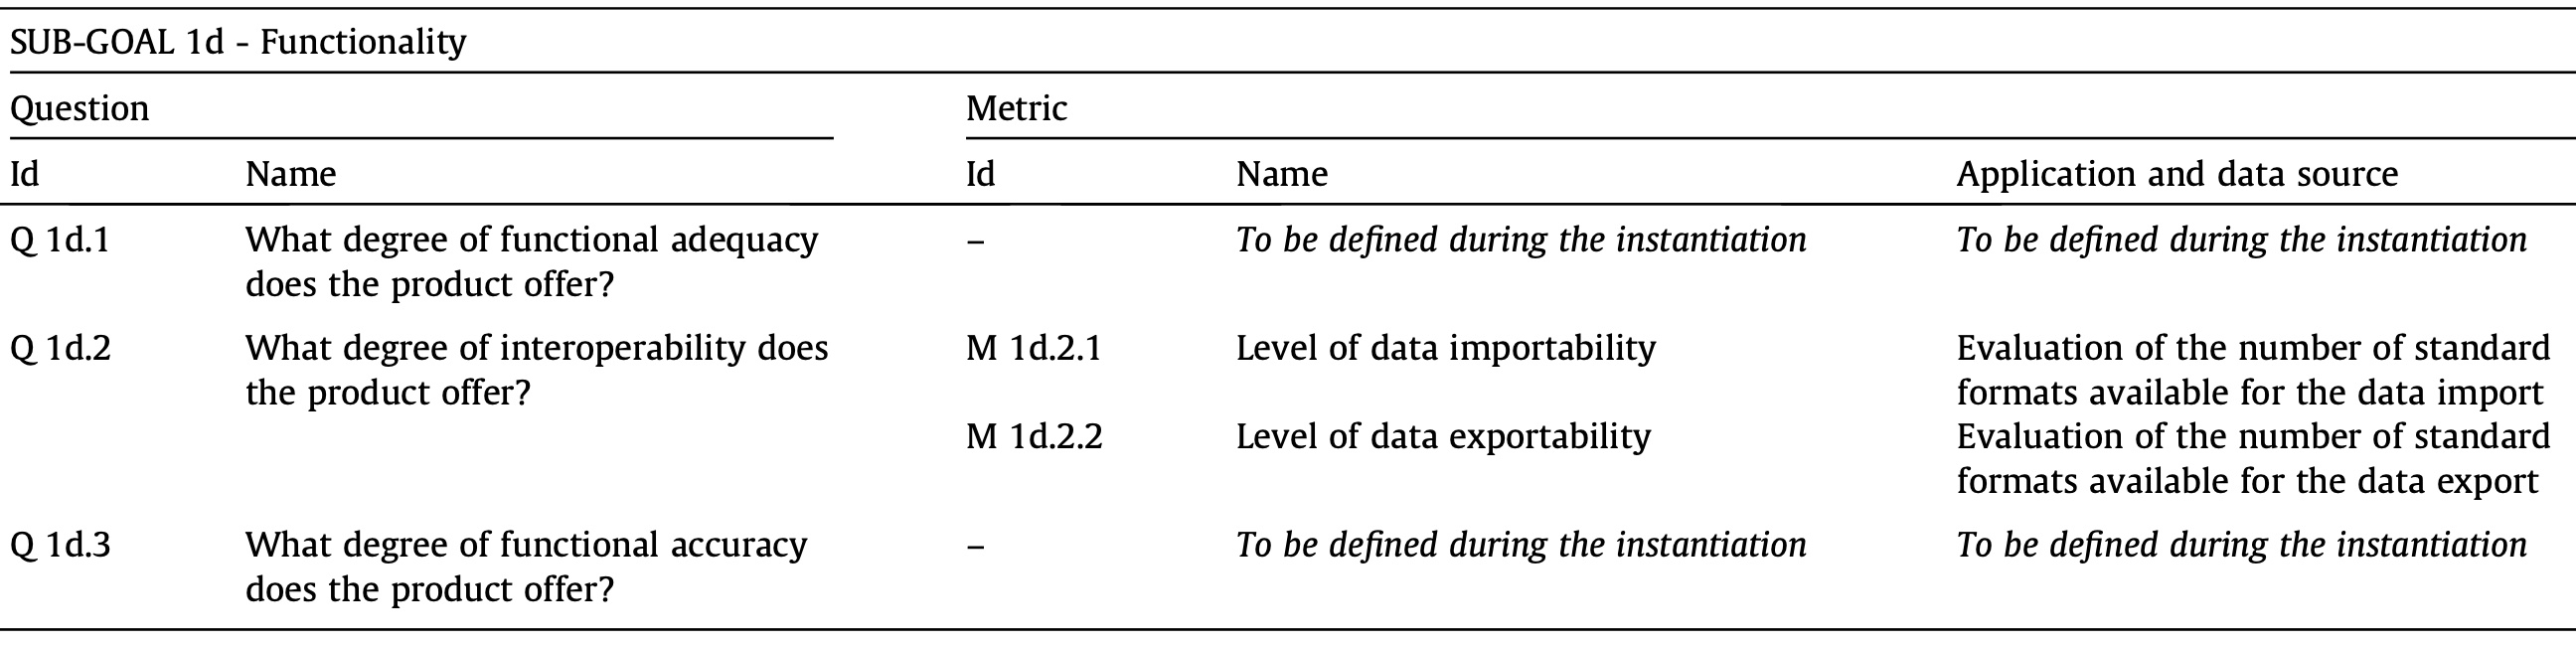
\includegraphics{images/table_5}
\caption{Questions and metrics in the EFFORT measurement framework pertaining Sub-goal 1d. Reproduced from~\cite{effort}}
\label{image_effort_table_5}
\end{figure}

\begin{figure}[h!]
\centering
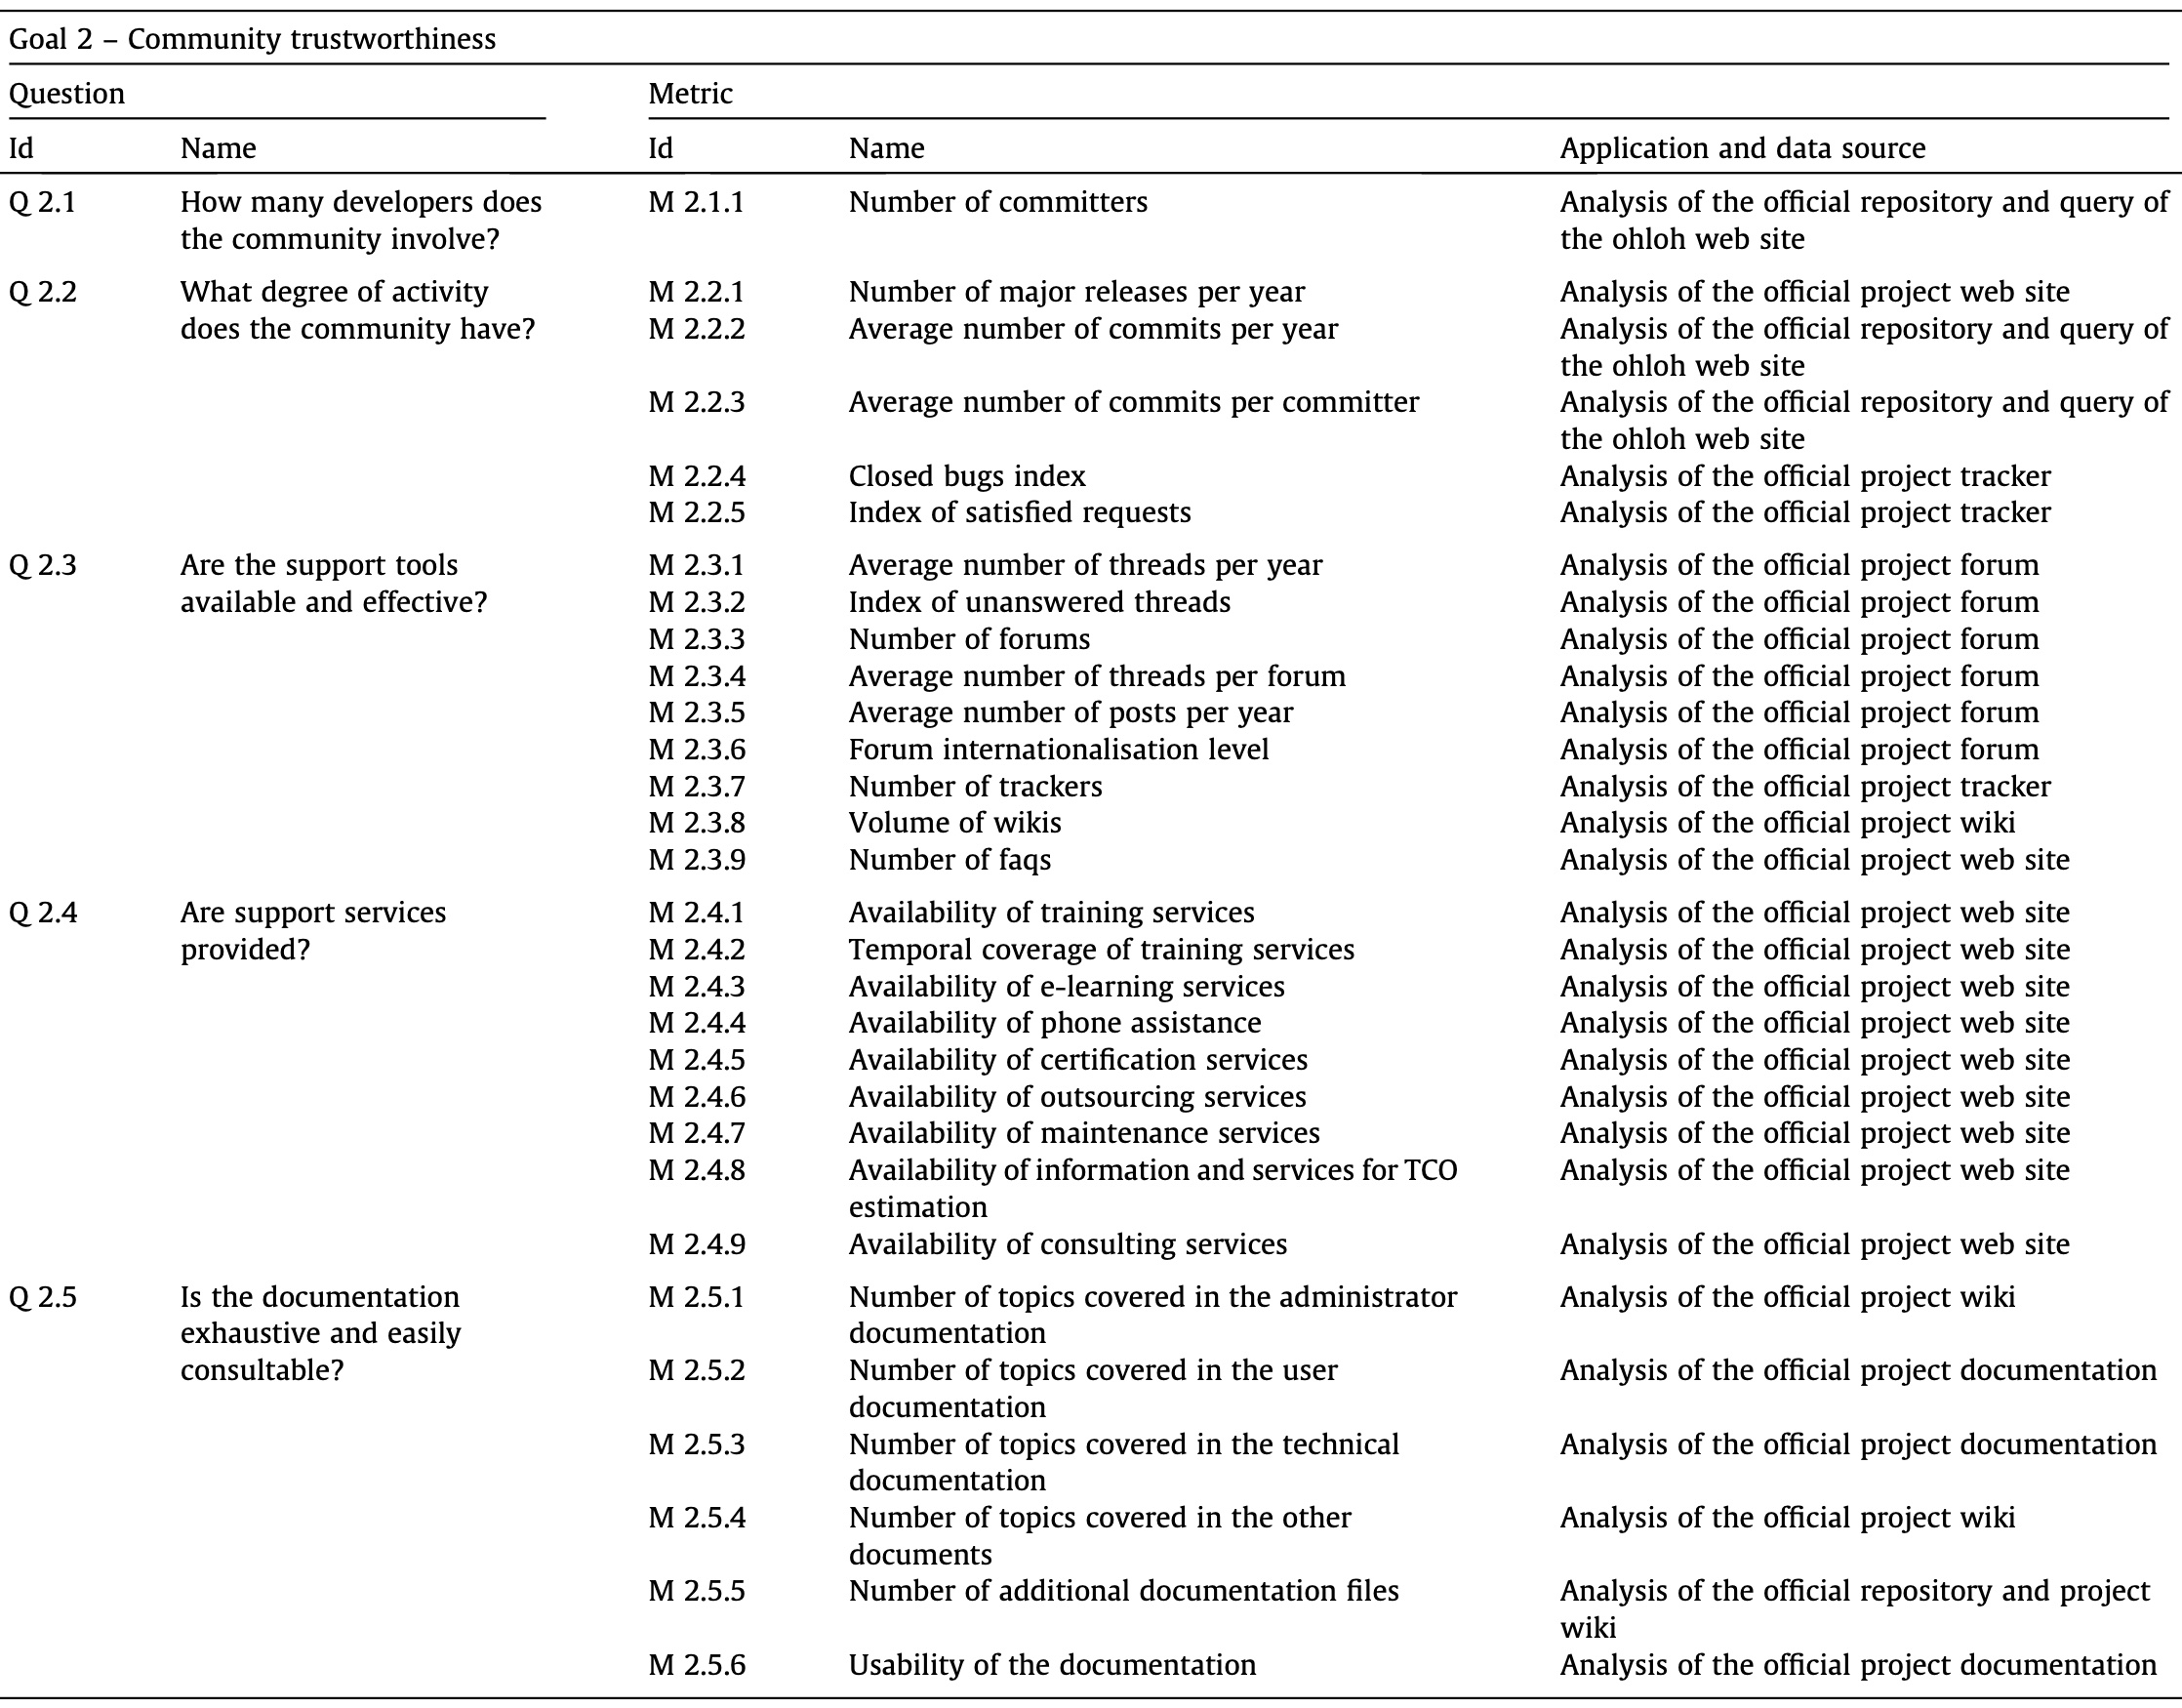
\includegraphics{images/table_6}
\caption{Questions in the EFFORT measurement framework pertaining to community trustworthiness. Reproduced from~\cite{effort}}
\label{image_effort_table_6}
\end{figure}

\begin{figure}[h!]
\centering
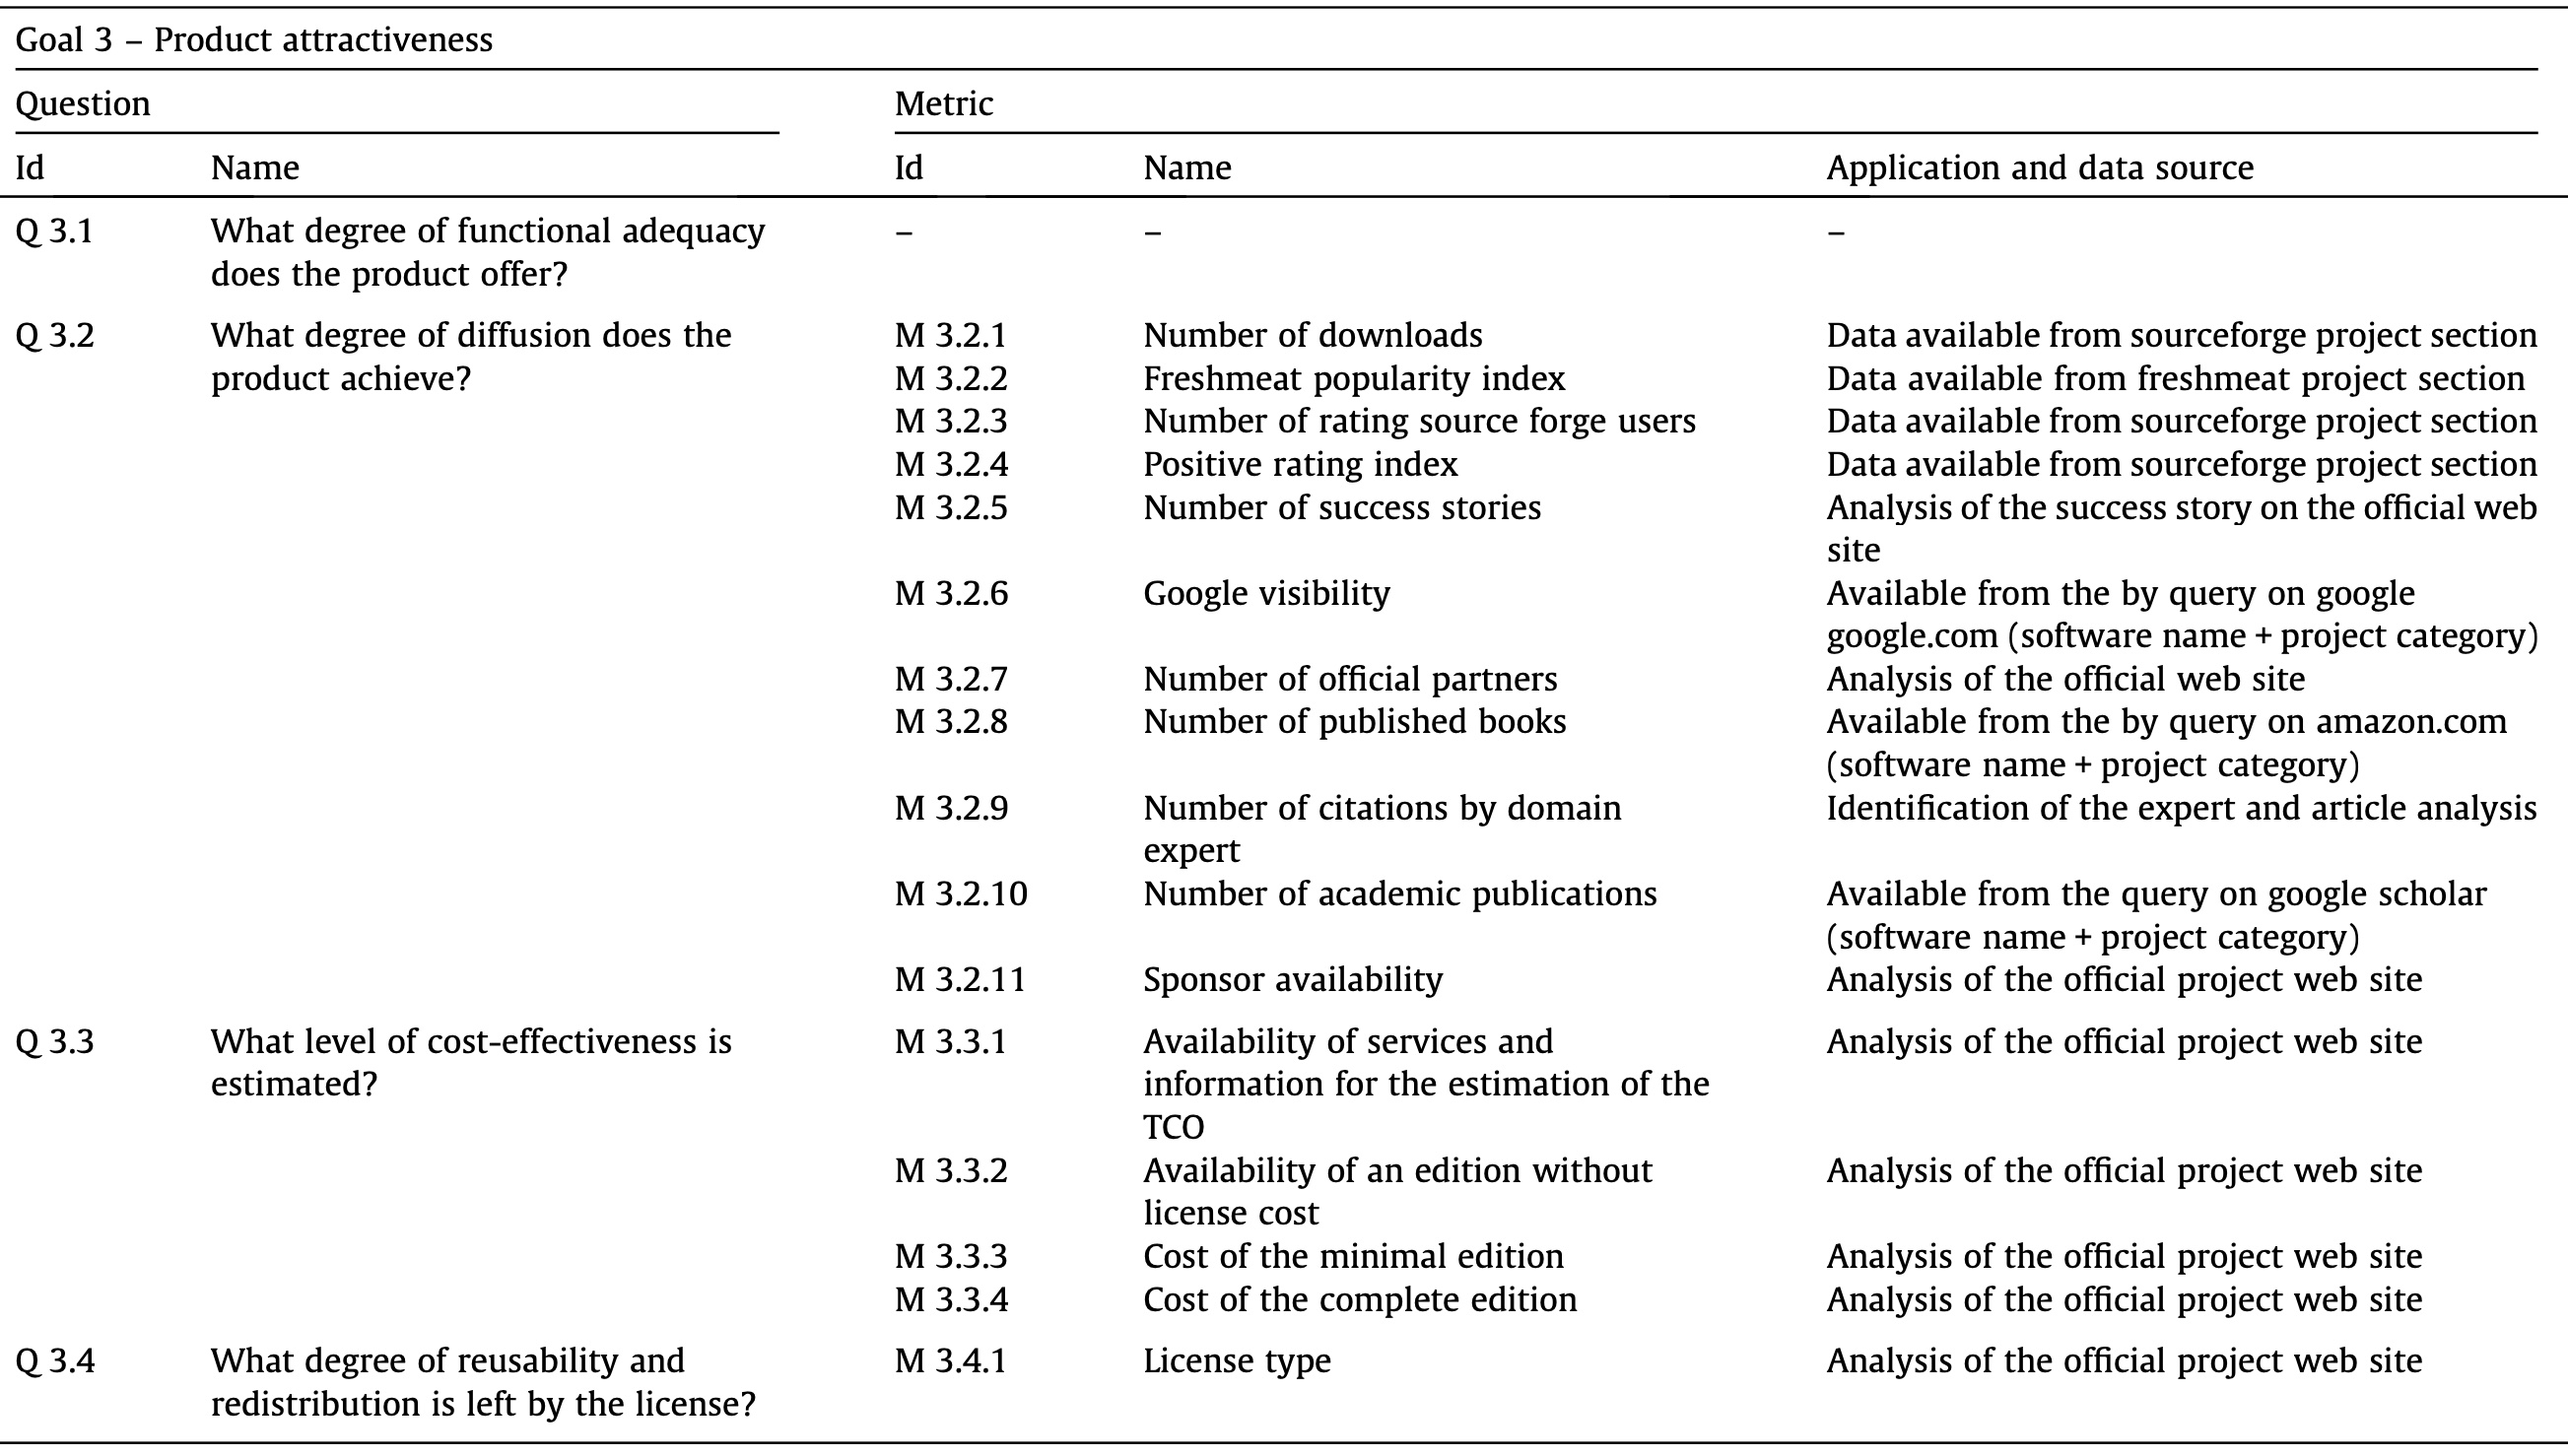
\includegraphics{images/table_7}
\caption{Questions in the EFFORT measurement framework pertaining to product attractiveness. Reproduced from~\cite{effort}}
\label{image_effort_table_7}
\end{figure}

As can be seen in figure ~\ref{image_effort_table_4} and ~\ref{image_effort_table_5},
some goals can't be completely defined in
a generic manner. Rather they need to be completed during the
instantiation process (see subsection \ref{instantiation-of-effort}).

Individual metrics can differ vastly. Whilst some may have a large
continuous scale, others may have unique enumerated possible values.
Therefore, each measurement is mapped to a discrete score ranging from 1
to 5, where 1 is interpreted as inadequate, 2 as poor, 3 as sufficient,
4 as good, and finally 5 as excellent. A higher value can also be
interpreted either positively or negatively, depending on the related
question. Therefore, a correct interpretation (positive or negative)
needs to be defined. Lastly, since different questions have different
importances within a goal, each question is assigned a relative
relevance.

\begin{minipage}{\textwidth}
Consequently, the quality of each goal can be calculated as
follows:

\[
q(g)=\frac{\Sigma_{q\in Q_q}r_q*m(q)}{\Sigma_{q\in Q_q}r_q}
\]

where \(r_q\) is the relevance associated with the question \(q\),
\(Q_g\) is the set of questions related to the Goal \(g\), and \(m(q)\)
is the aggregation function of the metrics of the question \(q\).
Essentially, the quality of a goal is defined by the weighted average of
its questions' scores.
\end{minipage}
\newpage
\begin{minipage}{\textwidth}
    The aggregation function of the metrics of a
    question \(q\) is defined as follow:

\[
    m(q)=\frac
    {\{\Sigma_{id\in M_q}
        i(id)*v(id)
        +[1-i(id)]
        *v(id)mod6]
        \}}
    {|M_q|}
\]

where \(v(id)\) is the value of the metric \(id\) and \(i(id)\) is the
interpretation of the metric with respect to the question \(q\) and has
the value of \(0\) if the metric has a negative interpretation and \(1\)
otherwise. \(M_q\) is the set of metrics related to a question \(q\).
    Simply put, the aggregation function is the average score obtained by
    its metrics, whereas if the metric is negatively interpreted, its
    complement is taken.
\end{minipage}


In this work, \(mod6\) is
interpreted as the metric's complement within the given metrics range
\([1-5]\) and not the modulo, since using the modulo would simply return the same value,
as displayed in figure~\ref{table_comparing_modulo}.
\newpage

\begin{figure}
\begin{longtable}[]{@{}lll@{}}
\toprule
Interpretation & Modulo \texttt{(n\%6)} & Metric complement \texttt{(6-n)} \\
\midrule
\endhead
1 & 1 & 5 \\
2 & 2 & 4 \\
3 & 3 & 3 \\
4 & 4 & 2 \\
5 & 5 & 1 \\
\bottomrule
\end{longtable}
\caption{Interpretation of $mod6$ as modulo and complement}
\label{table_comparing_modulo}
\end{figure}

Up until now, the presented goals, questions and metrics and their
relevance were based mainly on an Open Source Software point of view. As
previously stated, the EFFORT framework can be customized to suit the
context of its application. In the following chapter, the instantiation
of EFFORT is presented.

\clearpage
\hypertarget{instantiation-of-effort}{%
    \section{Instantiation of EFFORT}\label{instantiation-of-effort}}

The customization of EFFORT, i.e.~its binding to a concrete use case, is
achieved through three steps~\cite{effort}. First, the application domain
should be analyzed in order to gain thorough context specific knowledge
and understand the specific requirements. This has been done in chapter~\ref{conceptual-background}
of this work. Next, the collected information of the previous step
is used to verify the validity of the questions of the EFFORT baseline
version. In the third step, additional questions and metrics can be
added to better match the application domain~\cite{effort}.

Following, the second and third step of the customization of EFFORT are
presented. Although the third step can be split between integration
tasks, where metrics are added to the baseline versions and extension
tasks, where goals are extended by adding questions, these two steps are
presented at once by iterating over the goals which contributes to an
improved comprehensibility as there is no need to switch back and forth
between different topics. The resulting definition of questions and
metrics including interpretation of the metrics, their mapping from a raw
value to the given scale of \([1-5]\), and the questions' relevance
are to be found in the appendix~\ref{appendix_a_effort_instantiation}.


%%\setlength\tabcolsep{2pt}
%\caption{My caption}
%\label{lbl}
\begin{tabular}[]{|p{1cm}p{2cm}p{1.5cm}p{1.5cm}p{5cm}p{2.5cm}|}

Q-Id & Question & Q-State & M-Id & Metric & M-state \\
\hline
    \hline
1a.1 & Adaptability & KEPT & 1a.1.1 & Number of operating systems
supported & REMOVED \\
& & & 1a.1.2 & Support for Function and Class Components & ADDED \\
& & & 1a.1.3 & Adoption of React Suspense & ADDED \\
1a.2 & Installability & KEPT & 1a.2.1 & Time required for installation &
REMOVED \\
& & & 1a.2.2 & Availability of the installation manual & KEPT \\
& & & 1a.2.3 & Automation level and use of installation scripts &
REMOVED \\
& & & 1a.2.4 & Dependence on third-party components & KEPT \\
& & & 1a.2.5 & Nominal length of the installation procedures &
REMOVED \\
& & & 1a.2.6 & Number of configuration files Minimum number of files
added and changed for minimum functionality & CHANGED \\
& & & 1a.2.7 & Availability and rationality of default options &
CHANGED \\
& & & 1a.2.8 & Internationalisation of the manual & KEPT \\
& & & 1a.2.9 & Number of unforeseen issues & KEPT \\
& & & 1a.2.10 & Degree of knowledge of the required operating
environment & KEPT \\
& & & 1a.2.11 & Efficacy of the guide & KEPT \\
1a.3 & Replaceability & KEPT & 1a.3.1 & Existence of other libraries
with the same functionality and a similar API & ADDED \\
1a.4 & Coexistence & REMOVED & & & \\
\end{tabular}

%\begin{longtable}[]{@{}llllllll@{}}
\toprule
GoalId & Goal & QuestionId & Question & QuestionState & MetricId &
Metric & Metric state \\
\midrule
\endhead
1a & Portability & 1a.1 & Adaptability & KEPT & 1a.1.1 & Number of
operating systems supported & REMOVED \\
& & & & & 1a.1.2 & Support for Function and Class Components & ADDED \\
& & & & & 1a.1.3 & Adoption of React Suspense & ADDED \\
& & 1a.2 & Installability & KEPT & 1a.2.1 & Time required for
installation & REMOVED \\
& & & & & 1a.2.2 & Availability of the installation manual & KEPT \\
& & & & & 1a.2.3 & Automation level and use of installation scripts &
REMOVED \\
& & & & & 1a.2.4 & Dependence on third-party components & KEPT \\
& & & & & 1a.2.5 & Nominal length of the installation procedures &
REMOVED \\
& & & & & 1a.2.6 & Number of configuration files Minimum number of files
added and changed for minimum functionality & CHANGED \\
& & & & & 1a.2.7 & Availability and rationality of default options &
CHANGED \\
& & & & & 1a.2.8 & Internationalisation of the manual & KEPT \\
& & & & & 1a.2.9 & Number of unforeseen issues & KEPT \\
& & & & & 1a.2.10 & Degree of knowledge of the required operating
environment & KEPT \\
& & & & & 1a.2.11 & Efficacy of the guide & KEPT \\
& & 1a.3 & Replaceability & KEPT & 1a.3.1 & Existence of other libraries
with the same functionality and a similar API & ADDED \\
& & 1a.4 & Coexistence & REMOVED & & & \\
1b & Maintainability & 1b.1 & Analyzability & KEPT & 1b.1.1 &
Availability and quality of developer tools & ADDED \\
& & 1b.2 & Changeability & REMOVED & & // because libraries cannot be
changed by definition & \\
& & 1b.3 & Testability & KEPT & 1b.3.1 & Possibility to test business
logic without React & ADDED \\
& & 1b.4 & Technology concentration & REMOVED & & // ambiguous term:
"Technology concentration" & \\
& & 1b.5 & Stability & KEPT & 1b.5.1 & Breaking API changes & ADDED \\
& & 1b.6 & How maintainable is the application code using the product? &
ADDED & 1b.6.1 & Code duplication & ADDED \\
& & & & & 1b.6.2 & Cyclomatic complexity & ADDED \\
& & & & & 1b.6.3 & Cognitive complexity & ADDED \\
\bottomrule
\end{longtable}

%\begin{longtable}[]{@{}llllllll@{}}
\toprule
GoalId & Goal & QuestionId & Question & QuestionState & MetricId &
Metric & Metric state \\
\midrule
\endhead
1c & Reliability & 1c.1 & Rebustness & REMOVED & & // non applicable to
domain & \\
& & 1c.2 & Recoverability & REMOVED & & // non applicable to domain & \\
1d & Functionallity & 1d.1 & Functional adequacy & KEPT & 1d.1.1 &
Possibility to share state without prop drilling. & ADDED \\
& & & & & 1d.1.2 & Possibility to have derived state. & ADDED \\
& & 1d.2 & Interoperability & KEPT & 1d.2.1 & Level of data
importability & REMOVED \\
& & & & & 1d.2.2 & Level of data exportability & REMOVED \\
& & & & & 1d.2.3 & Availability of community plugins & ADDED \\
& & 1d.3 & Functional accuracy & KEPT & 1d.3.1 & Lines of code &
ADDED \\
& & & & & 1d.3.2 & Statement count & ADDED \\
& & & & & 1d.3.3 & Functions count & ADDED \\
1e & Usability & 1e.1 & Pleasantness & REMOVED & & // non applicable to
domain & \\
& & 1e.2 & Operability & KEPT & 1e.2.1 & Availability and quality of
developer tools (same as 1b.1.1) & ADDED \\
& & 1e.3 & Understandability & REMOVED & & // non applicable to domain
& \\
& & 1e.4 & Learnability & KEPT & - & Same metrics as in Question 2.5 &
ADDED \\
1f & Efficiency & 1f.1 & Time behavior & KEPT & 1f.1.1 & First
Contentful Paint & ADDED \\
& & & & & 1f.1.2 & Speed Index & ADDED \\
& & & & & 1f.1.3 & Largest Contentful Paint & ADDED \\
& & & & & 1f.1.4 & Time to Interactive & ADDED \\
& & & & & 1f.1.5 & Total Blocking Time & ADDED \\
& & & & & 1f.1.6 & Cumulative Layout Shift & ADDED \\
& & 1f.2 & Resources utilization & KEPT & 1f.2.1 & Efficient re-renders
& ADDED \\
\bottomrule
\end{longtable}

%\begin{longtable}[]{@{}llllll@{}}
\toprule
QuestionId & Question & QuestionState & MetricId & Metric & Metric
state \\
\midrule
\endhead
2.1 & How many developers does the community involve? & KEPT & 2.1.1 &
Number of committers & KEPT \\
2.2 & What degree of activity does the community have? & KEPT & 2.2.1 &
Number of major releases per year & REMOVED \\
& & & 2.2.2 & Average number of commits per year & KEPT \\
& & & 2.2.3 & Average number of commits per committer & KEPT \\
& & & 2.2.4 & Closed bugs index issues on GitHub & CHANGED \\
& & & 2.2.5 & Index of satisfied requests merged pull requests on GitHub
& CHANGED \\
2.3 & Are the support tools available and effective? & KEPT & 2.3.1 &
Average number of threads per year on StackOverflow & KEPT \\
& & & 2.3.2 & Index of unanswered threads on StackOverflow & KEPT \\
& & & 2.3.3 & Number of forums & REMOVED \\
& & & 2.3.4 & Average number of threads per forum & REMOVED \\
& & & 2.3.5 & Average number of posts per year & REMOVED \\
& & & 2.3.6 & Forum internationalisation level & REMOVED \\
& & & 2.3.7 & Number of trackers & REMOVED \\
& & & 2.3.8 & Volume of Wikis Usability of the documentation (same as
2.5.6) & CHANGED \\
& & & 2.3.9 & Number of faqs in the documentation & CHANGED \\
2.4 & Are support services provided? & KEPT & 2.4.1 & Availability of
training services & KEPT \\
& & & 2.4.2 & Temporal coverage of training services & REMOVED \\
& & & 2.4.3 & Availability of e-learning services & REMOVED \\
& & & 2.4.4 & Availability of phone assistance & REMOVED \\
& & & 2.4.5 & Availability of certification services & KEPT \\
& & & 2.4.6 & Availability of outsourcing services & REMOVED \\
& & & 2.4.7 & Availability of maintenance services & REMOVED \\
& & & 2.4.8 & Availability of information and services for TCO
estimation & REMOVED \\
& & & 2.4.9 & Availability of consulting services & KEPT \\
2.5 & Is the documentation exhaustive and easily consultable? & KEPT &
2.5.1 & Number of topics covered in the administrator documentation &
REMOVED \\
& & & 2.5.2 & Number of topics covered in the user documentation &
REMOVED \\
& & & 2.5.3 & Number of topics covered in the technical documentation &
REMOVED \\
& & & 2.5.4 & Number of topics covered in the other documents &
REMOVED \\
& & & 2.5.5 & Number of additional documentation files & REMOVED \\
& & & 2.5.6 & Usability of the documentation & KEPT \\
\bottomrule
\end{longtable}

%\begin{longtable}[]{@{}llllll@{}}
\toprule
QuestionId & Question & QuestionState & MetricId & Metric & Metric
state \\
\midrule
\endhead
3.1 & What degree of functional adequacy does the product offer? & KEPT
& & // Same as 1d.1 & \\
& & & 3.2.1 & Number of weekly downloads & CHANGED \\
3.2 & What degree of diffusion does the product achieve? & KEPT & 3.2.2
& Freshmeat popularity index Number of stars on GitHub & CHANGED \\
& & & 3.2.3 & Number of rating source forge users Number of forks on
GitHub & CHANGED \\
& & & 3.2.4 & Positive rating index & REMOVED \\
& & & 3.2.5 & Number of success stories & REMOVED \\
& & & 3.2.6 & Google visibility & REMOVED \\
& & & 3.2.7 & Number of official partners/spronsors & CHANGED \\
& & & 3.2.8 & Number of published books & KEPT \\
& & & 3.2.9 & Number of citations by domain expert & REMOVED \\
& & & 3.2.10 & Number State of academic publications & CHANGED \\
& & & 3.2.11 & Sponsor availability & KEPT \\
3.3 & What level of cost-effectiveness is estimated? & REMOVED & 3.3.1 &
Availability of services and information for the estimation of the TCO &
REMOVED \\
& & & 3.3.2 & Availability of an edition without license cost &
REMOVED \\
& & & 3.3.3 & Cost of the minimal edition & REMOVED \\
& & & 3.3.4 & Cost of the complete edition & REMOVED \\
3.4 & What degree of reusability and redistribution is left by the
license? & KEPT & 3.4.1 & License type & KEPT \\
\bottomrule
\end{longtable}


Upon analyzing the application context along with the baseline EFFORT
goals, questions and metrics, it could be established that the proposed
questions are mostly sufficient. The only question that has been added is
``How maintainable is the application code using the product?''(1b.6) in the
goal Maintainability (1b). Moreover, only
a few questions have been removed due to their inapplicability in the
given domain.
Within the first sub-Goal `Portability' (1a), the question related to
`Coexistence' (1a.4) has been removed due to its irrelevance. Within the
question (1a.1) regarding Adaptability, the metric `Number of operating systems supported' has
been replaced by `Support for Function and Class Components'(1a.1.2) ,
and `Adoption of React Suspense'(1a.1.3), which is an upcoming React
feature~\cite{react_suspense}. Since the libraries can be easily installed with a
package manager such as npm~\cite{npm}, multiple metrics of the question related to
`Installability' (1a.2) have been left out.
Moreover, the `Number of configuration files' (1a.2.6) has been replaced
by the `Minimum number of files added and changed for minimum
functionality'. Additionally, the `Availability of default options'
(1a.2.7) has been extended to include their rationality. In order to
measure `Replaceability', the metric `Existence of other libraries with
the same functionality and a similar API' (1a.3.1) has been introduced.

Within the `Maintainability goal' (1b.2), `Changeability' was considered
irrelevant, since libraries cannot be changed by definition.
Furthermore, the question regarding `Technology Concentration' is
excluded due to its ambiguity. In order to measure the `Analyzability',
multiple metrics have been added among others `Availability and quality
of developer tools'. Besides, `Stability' is measured by the `Existence
and degree of Breaking API changes' and `Testability' is assessed by the
`Possibility to test business logic without React'. The question `How
maintainable is the application code using the software product?' (1b.6)
is introduced and it consists of the metrics `Code duplication',
`Cyclomatic complexity'~\cite{cyclomatic_complexity} and `Cognitive complexity'\cite{cognitive_complexity}. Cognitive
complexity is a measurement, that attempts to ``reflect the relative
difficulty of understanding the source code''~\cite{cognitive_complexity}. While formulating these metrics, it was assumed, that a
more suitable library would result in simpler and less source code in
general.

The goal `Reliability' that includes questions about `Robustness' and
`Recoverability', is considered irrelevant in this use-case. The
sub-goal `Functionality' is based on the problems presented in section. Thereby, two metrics are attributed to the question `Functional
adequacy', namely `The possibility to share state without prop drilling'
and `The possibility to have derived state'. The metrics of
`Interoperability' have been adjusted as well. Instead of measuring the
level of `Data importability'(1d.2.1) and `Data exportability'(1d.2.2), the
`Availability of community plugins' is adopted as a unique metric. In
addition, the metrics `Lines of code', `Statement count', and `Function
count' are introduced in order to measure the `Functional accuracy'. It
is worth mentioning, that these metrics refer to the source code of the
implementation of the use case formulated in the section~\ref{problem-use-case} while using the
libraries, and not the source code of the libraries itself. Once again,
less code is interpreted as a sign of higher suitability.

Regarding the sub-goal `Usability', the metric `Availability and quality
of developer tools' is used to measure the degree of `Operability'
whereas the `Learnability' is measured by looking at the degree of
`Usability of the documentation'. `Usability of the documentation' takes
into account whether installation instructions, a project setup, a hello
world example, and advanced guides are provided.

In order to measure the `Efficiency', the two questions of `Time
behavior' and `Resources utilization' are extended. The metrics of `Time
behavior' measure the loading speed of a webpage and include
the `First Contentful Paint'~\cite{first_contentful_paint},
the `Speed Index'~\cite{speed_index},
the `Largest Contentful Paint'~\cite{largest_contentful_paint},
the `Time to Interactive'~\cite{time_to_interactive},
the `Total Blocking Time'~\cite{total_blocking_time}, and the
`Cumulative Layout Shift'~\cite{cumulative_layout_shift}.
For measuring the
`Resource utilization', the problem of unnecessary re-renderings (P4)
presented above is used.

In order to evaluate the `Community
trustworthiness', multiple metrics are changed. First, the metric
`Number of major releases per year' is removed, since it can be
differently interpreted. Nevertheless, a few metrics have been adjusted
and others are removed namely `Number of forums', because the major
forum used is Stack Overflow.

Other metrics proposed by the EFFORT baseline version have been left out
due to their inapplicability to libraries, among others `Availability of
outsourcing services', `Availability of maintenance services',
`Availability of information and services for TCO estimation', and
`Temporal coverage of training services'. Also, since the
differentiation between administrator, user, technical, and other
documentations is not applicable in the context of libraries, metrics
related to the mentioned documentations are removed.

When it comes to `Product attractiveness', two factors play a role.
First, the libraries are free of cost and second, the libraries' source
code is available at GitHub.
Additionally, the number of downloads has been adjusted to weekly
downloads to match the stats available
from ``npm.com''~\cite{npm}.

\hypertarget{discussion}{%
    \chapter{Discussion}\label{discussion}}


In this chapter, the results of applying EFFORT are presented. Mainly
the resulting score of each approach is analyzed and more general
conclusions are drawn upon the suitability of each approach. Afterwards,
the hypotheses formulated in chapter section~\ref{motivation-and-hypotheses} are verified and a reflection
on the research process is presented.

\hypertarget{findings}{\section{Findings}\label{findings}}

\begin{figure}
    \centering
    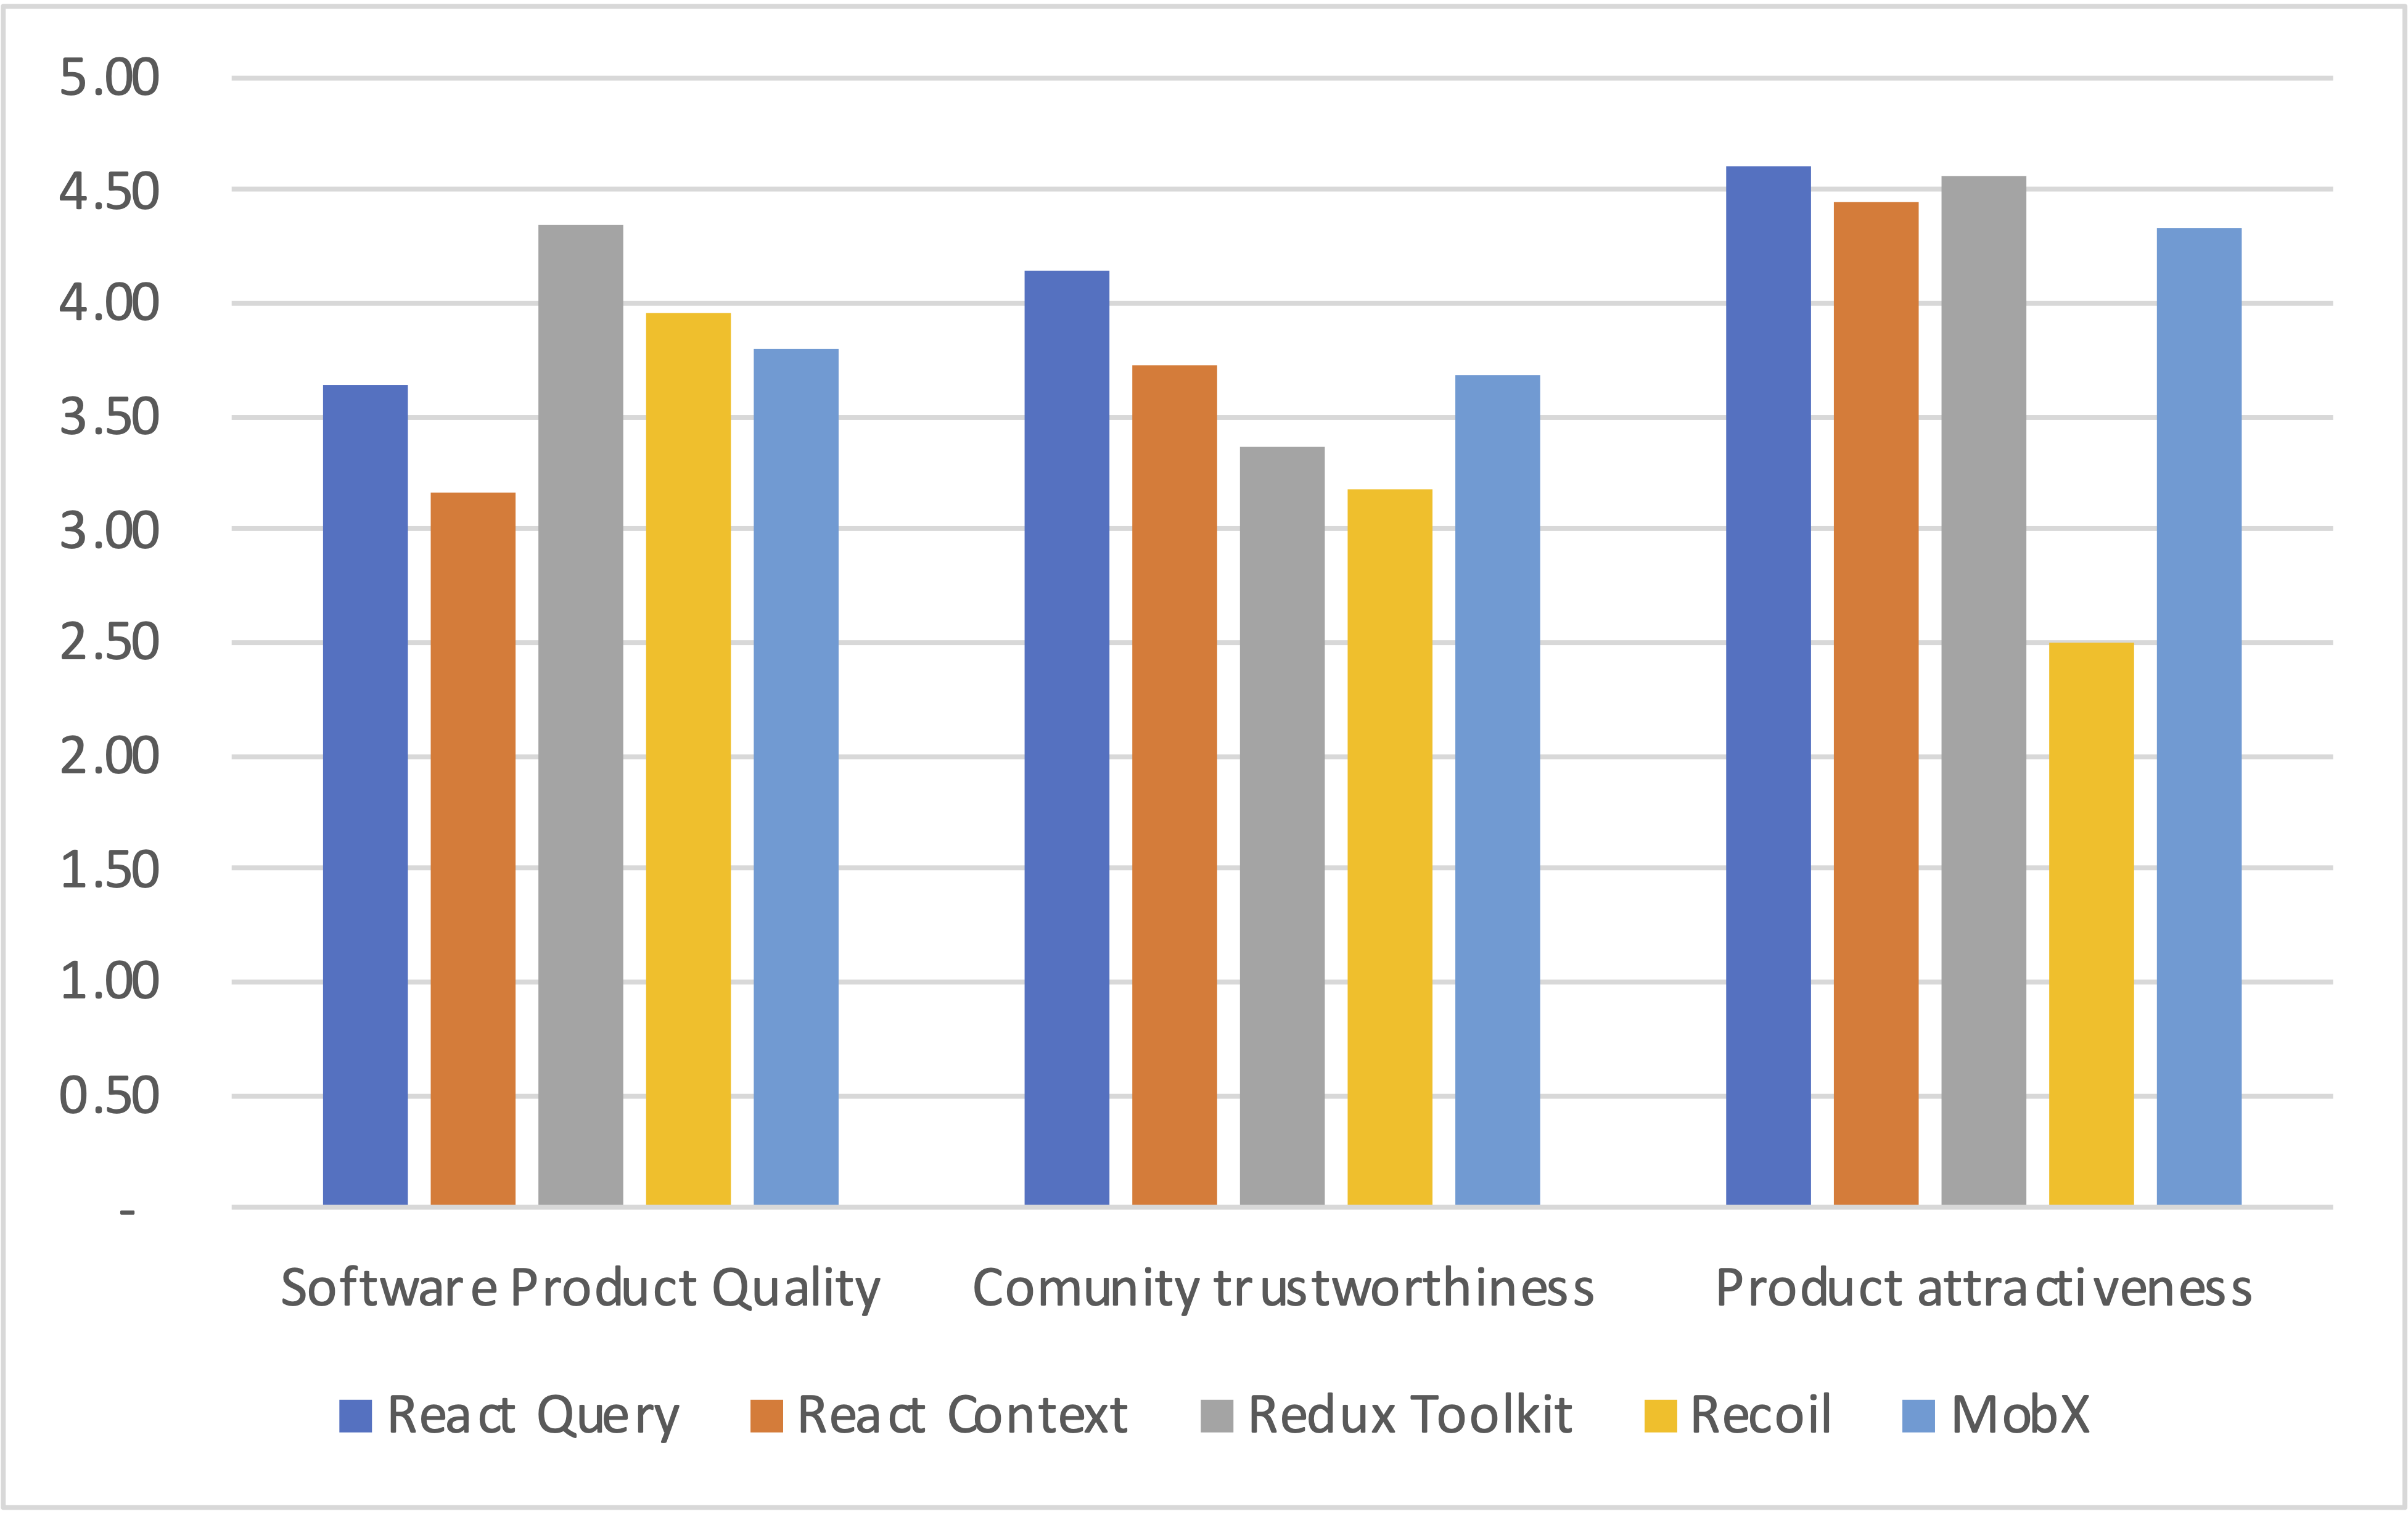
\includegraphics{images/overview}
    \caption{Scores achieved by the SMLs by applying EFFORT}
    \label{image_results_total}
\end{figure}

The results of the application of EFFORT on React Context, React Query,
Redux Toolkit, Recoil and MobX is shown in figure \ref{image_results_total}. A general
overview on the results shows that the approaches display varying levels
of `Software Product Quality', whereby React Context achieved the lowest
score. The `Community trustworthiness' has also varying results. Finally
the `Product attractiveness' is high in all the approaches with the
exception of Recoil which achieved a remarkably lower score. The scores
within each goal along with the influencing factors are explained further
in the following. The detailed scores achieved by each metric can be
found in the appendix \ref{appendix_b_results}.

\hypertarget{software-product-quality}{%
    \subsection{Software Product
    Quality}\label{software-product-quality}}

\begin{figure}
    \centering
    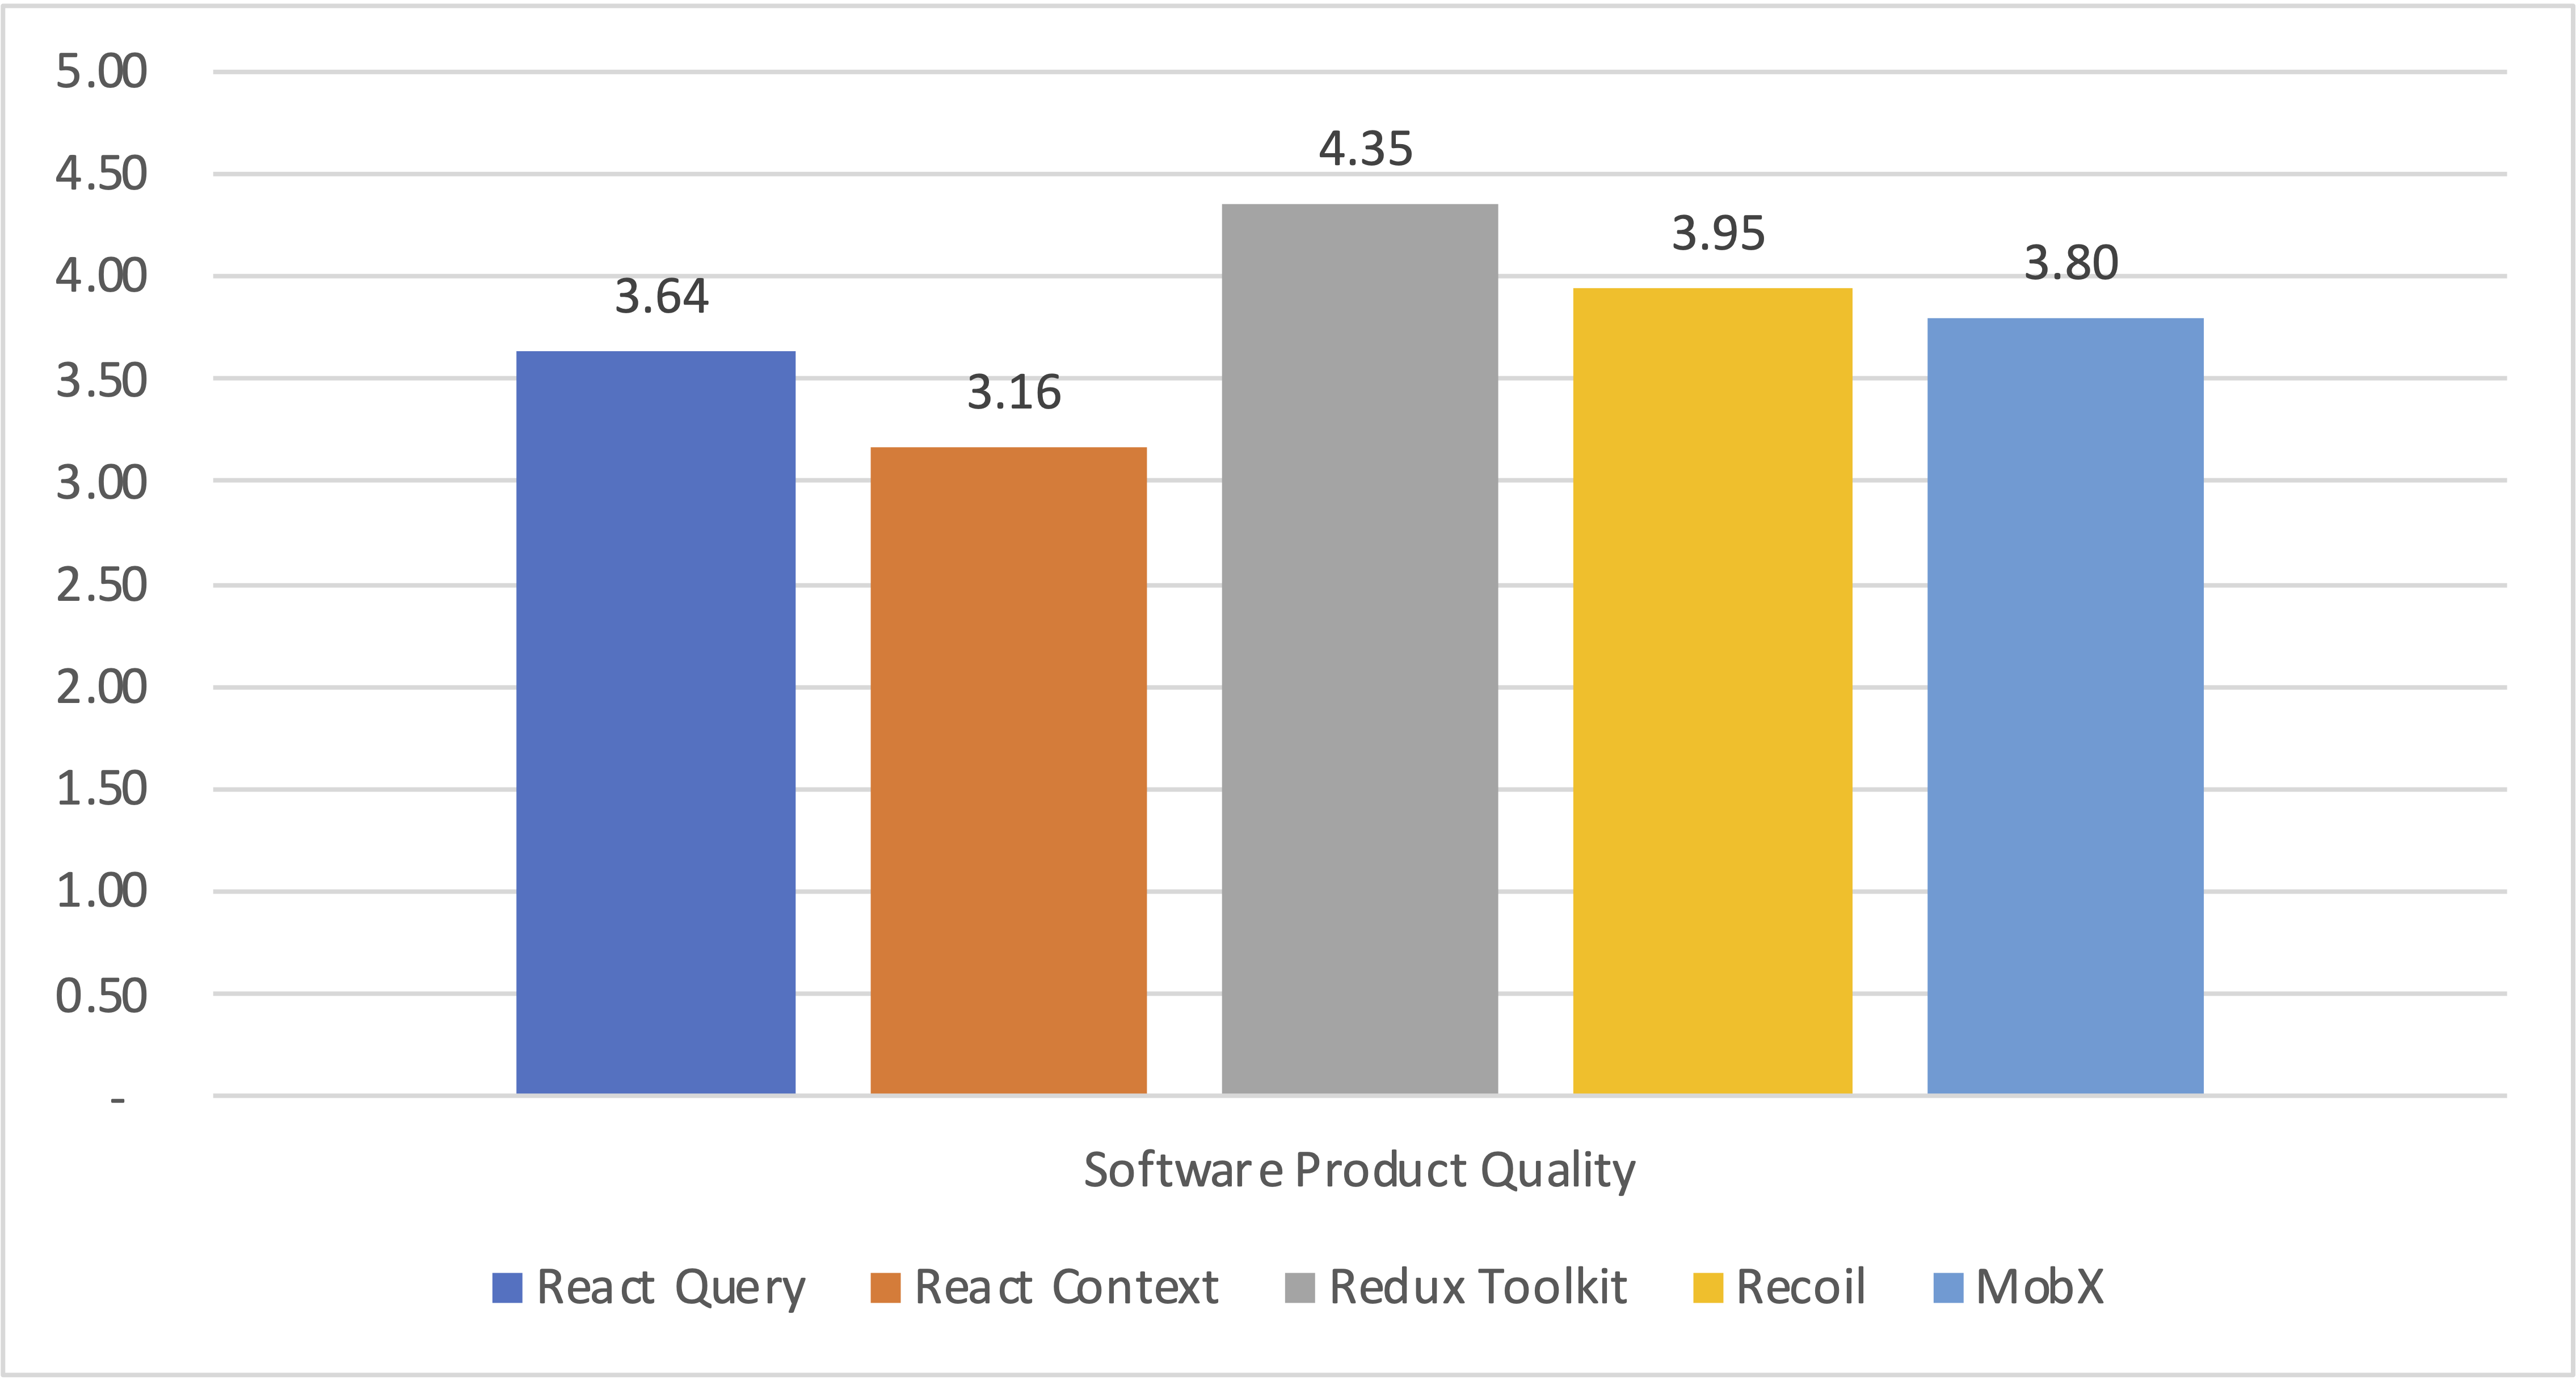
\includegraphics{images/chart_quality}
    \caption{Comparison of the software product quality of the five evaluated SMLs}
    \label{image_results_quality_general}
\end{figure}


Starting with the software product quality, the figure \ref{image_results_quality_general} presents the
results of the analyzed libraries where React Context exhibits the
lowest score. This is unsurprising, since React Context is a mechanism
whose only purpose is to solve the problem of prop drilling \cite{react_context}. On
the other hand, the first place is taken by Redux Toolkit. The high
score is due to the rich feature set of the library as well as its high
degree of `Testability'. Since Redux Toolkit is an opinionated library
that bases on Redux, it simplifies the definition of action
creators and async actions while retaining a high level of testability.
Additionally, its sub-package RTK Query covers the majority of React
Query's functionality. The second place belongs to Recoil and is
followed closely by MobX in the third position. Both of these libraries
benefit from efficient re-renderings. Moreover, testing
in both libraries can be done easily. Although it must be mentioned that
the use of the Object-Oriented Programming (OOP) by MobX simplifies the writing of code and the testing.
In contrast, Recoil solves common OOP problems with its atomic state
structure approach, most notably when having a complex dependencies in
the application state. React Query comes second to last. Although it
fulfills the requirements of managing server state, handling client
state exceeds the purpose of this library. Implementing client side
state requires using a global variable and invalidating the cache after
each change. This process is error prone and complicates the creation of
tests.

\begin{figure}
    \centering
    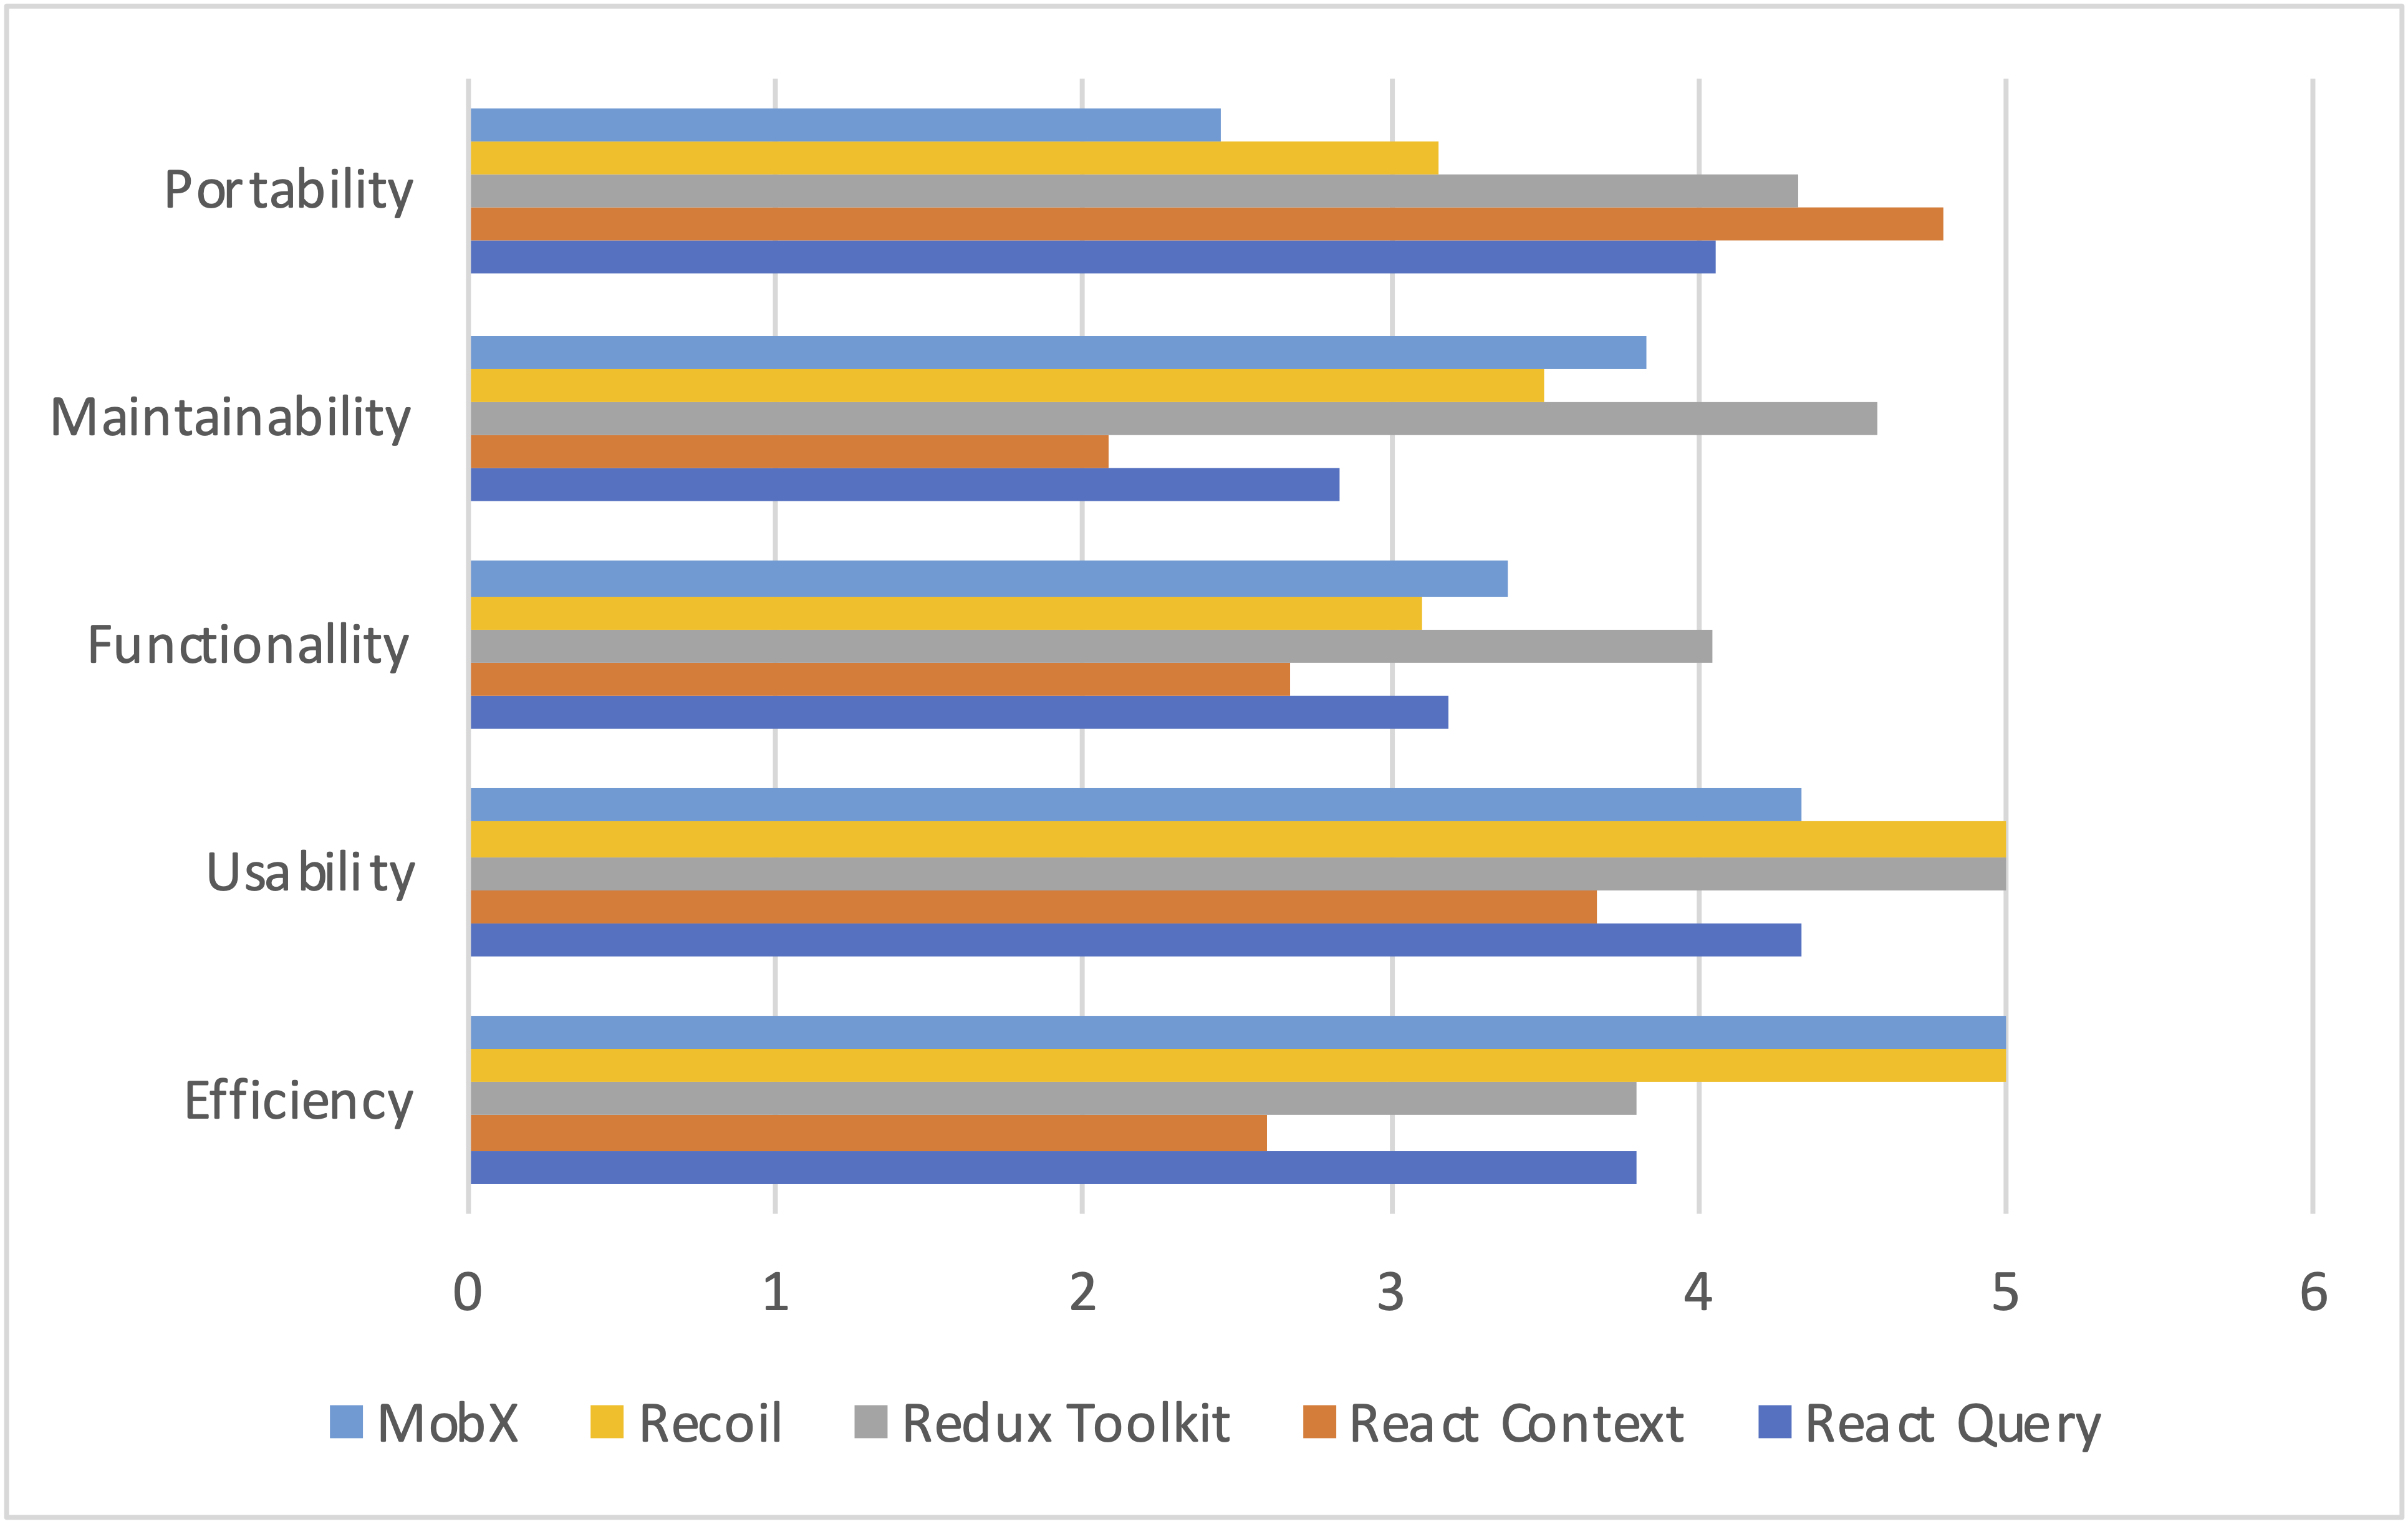
\includegraphics{images/chart_quality_details}
    \caption{Detailed results pertaining to the software product quality of the five evaluated SMLs}
    \label{image_results_quality_datailed}
\end{figure}

By analyzing the results of each subgoal of `Software Product Quality'
displayed in Figure \ref{image_results_quality_datailed}, a more elaborate understanding of the
differences between the libraries can be reached.

To begin with, the libraries show different degrees of `Portability'.
React Context's high degree of `Portability' comes from its support for
both function and class components and its support for React Suspense by definition, since it is part of the React library. Next come Redux Toolkit and React Query. While
React Query can be easily integrated into an existing application with
minimal additional code and file changes, Redux Toolkit supports both
class and function components (which is lacking in React Query and
Recoil) and the support for React Suspense is planned \cite{redux_toolkit_suspense_planned_support}. MobX
occupies the last place mainly due to its irreplaceability and lack of
default options. The replaceability was measured by the number of
libraries available that offer an equivalent functionality and a similar
API. While similar libraries exist for the rest, none could be found for
MobX. Additionally, MobX lacks a set of meaningful defaults, offering
the developer more flexibility and control, yet imposing the need to
write common code such as making API calls manually.

When it comes to maintainability, Redux Toolkit takes the lead. This is
directly caused by the high degree of testability and the sophisticated
developer tools provided~\cite{redux_dev_tools}. The testability of the code can be owed
to the clearly defined architecture that allows to run tests on
different layers. More importantly the use of pure functions in the
reducer and the selectors make it possible to write unit tests while
retaining the possibility of writing integration tests that include the
UI layer~\cite{redux_testing}. The developer tools provided for Redux Toolkit are
highly practical. Their key features include the possibility to browse
the history of the dispatched actions along with their effects on the
state, revert to a given state and the possibility to export and import
the complete state history~\cite{redux_dev_tools}. Next come React Query and Recoil, that both
include developer tools, yet with less functionality. React Query
surpasses Recoil in Stability. This is comprehensible, since at the time
of writing, Recoil is still in an experimental state \cite{recoil_github_experimental}.

Although there have been few breaking API changed introduced in React
Query, they included not only a migration guide, but a script that
applies the needed changes to the code using the library \cite{react_toolkit_upgrade_with_codemod}. On the
last place comes React Query mainly because of the difficulty of testing
it. While calculating the `Maintainability, other metrics were taken
into account such as `Code duplication', `Cyclomatic complexity' and
`Cognitive complexity', which are directly linked to the source code.
The libraries performed similarly in all of these measures and no
conclusions could be made in this regard.

Regarding `Functionality', all the libraries fulfill the requirements of
sharing the state without prop drilling and having a derived state.
Redux Toolkit receives the highest score because of its high degree of
`Interoperability' stemming from the large amount of plugins available,
an area which is lacked by others. It is followed by MobX, which
displayed a high degree of `Functional Adequacy', due to the low count
of lines, statement and functions needed to implement the same
functionality.

Redux Toolkit and Recoil show the highest level of usability. Thanks to
their documentations that include advanced guides and are translated to
multiple languages, the libraries excel in `Learnability'. Their ease of
`Operability' comes from having high quality developer tools.

Lastly, Efficiency was strongly influenced by `Effectiveness of the
re-rendering of the components', since all the libraries achieved
similar high score related the loading page speed. That is to say that the
choice of these libraries does not seem to have any effect on the loading speed
of the application whatsoever. Within the `Efficiency of re-rendering'
, Recoil and MobX have shown efficient
re-renderings, Redux Toolkit and React Query suboptimal re-renderings and
React Context redundant re-renderings (see section~\ref{problem-definition} for a definition of the terms).

\hypertarget{community-trustworthiness}{%
    \subsection{Community
    Trustworthiness}\label{community-trustworthiness}}

\begin{figure}
    \centering
    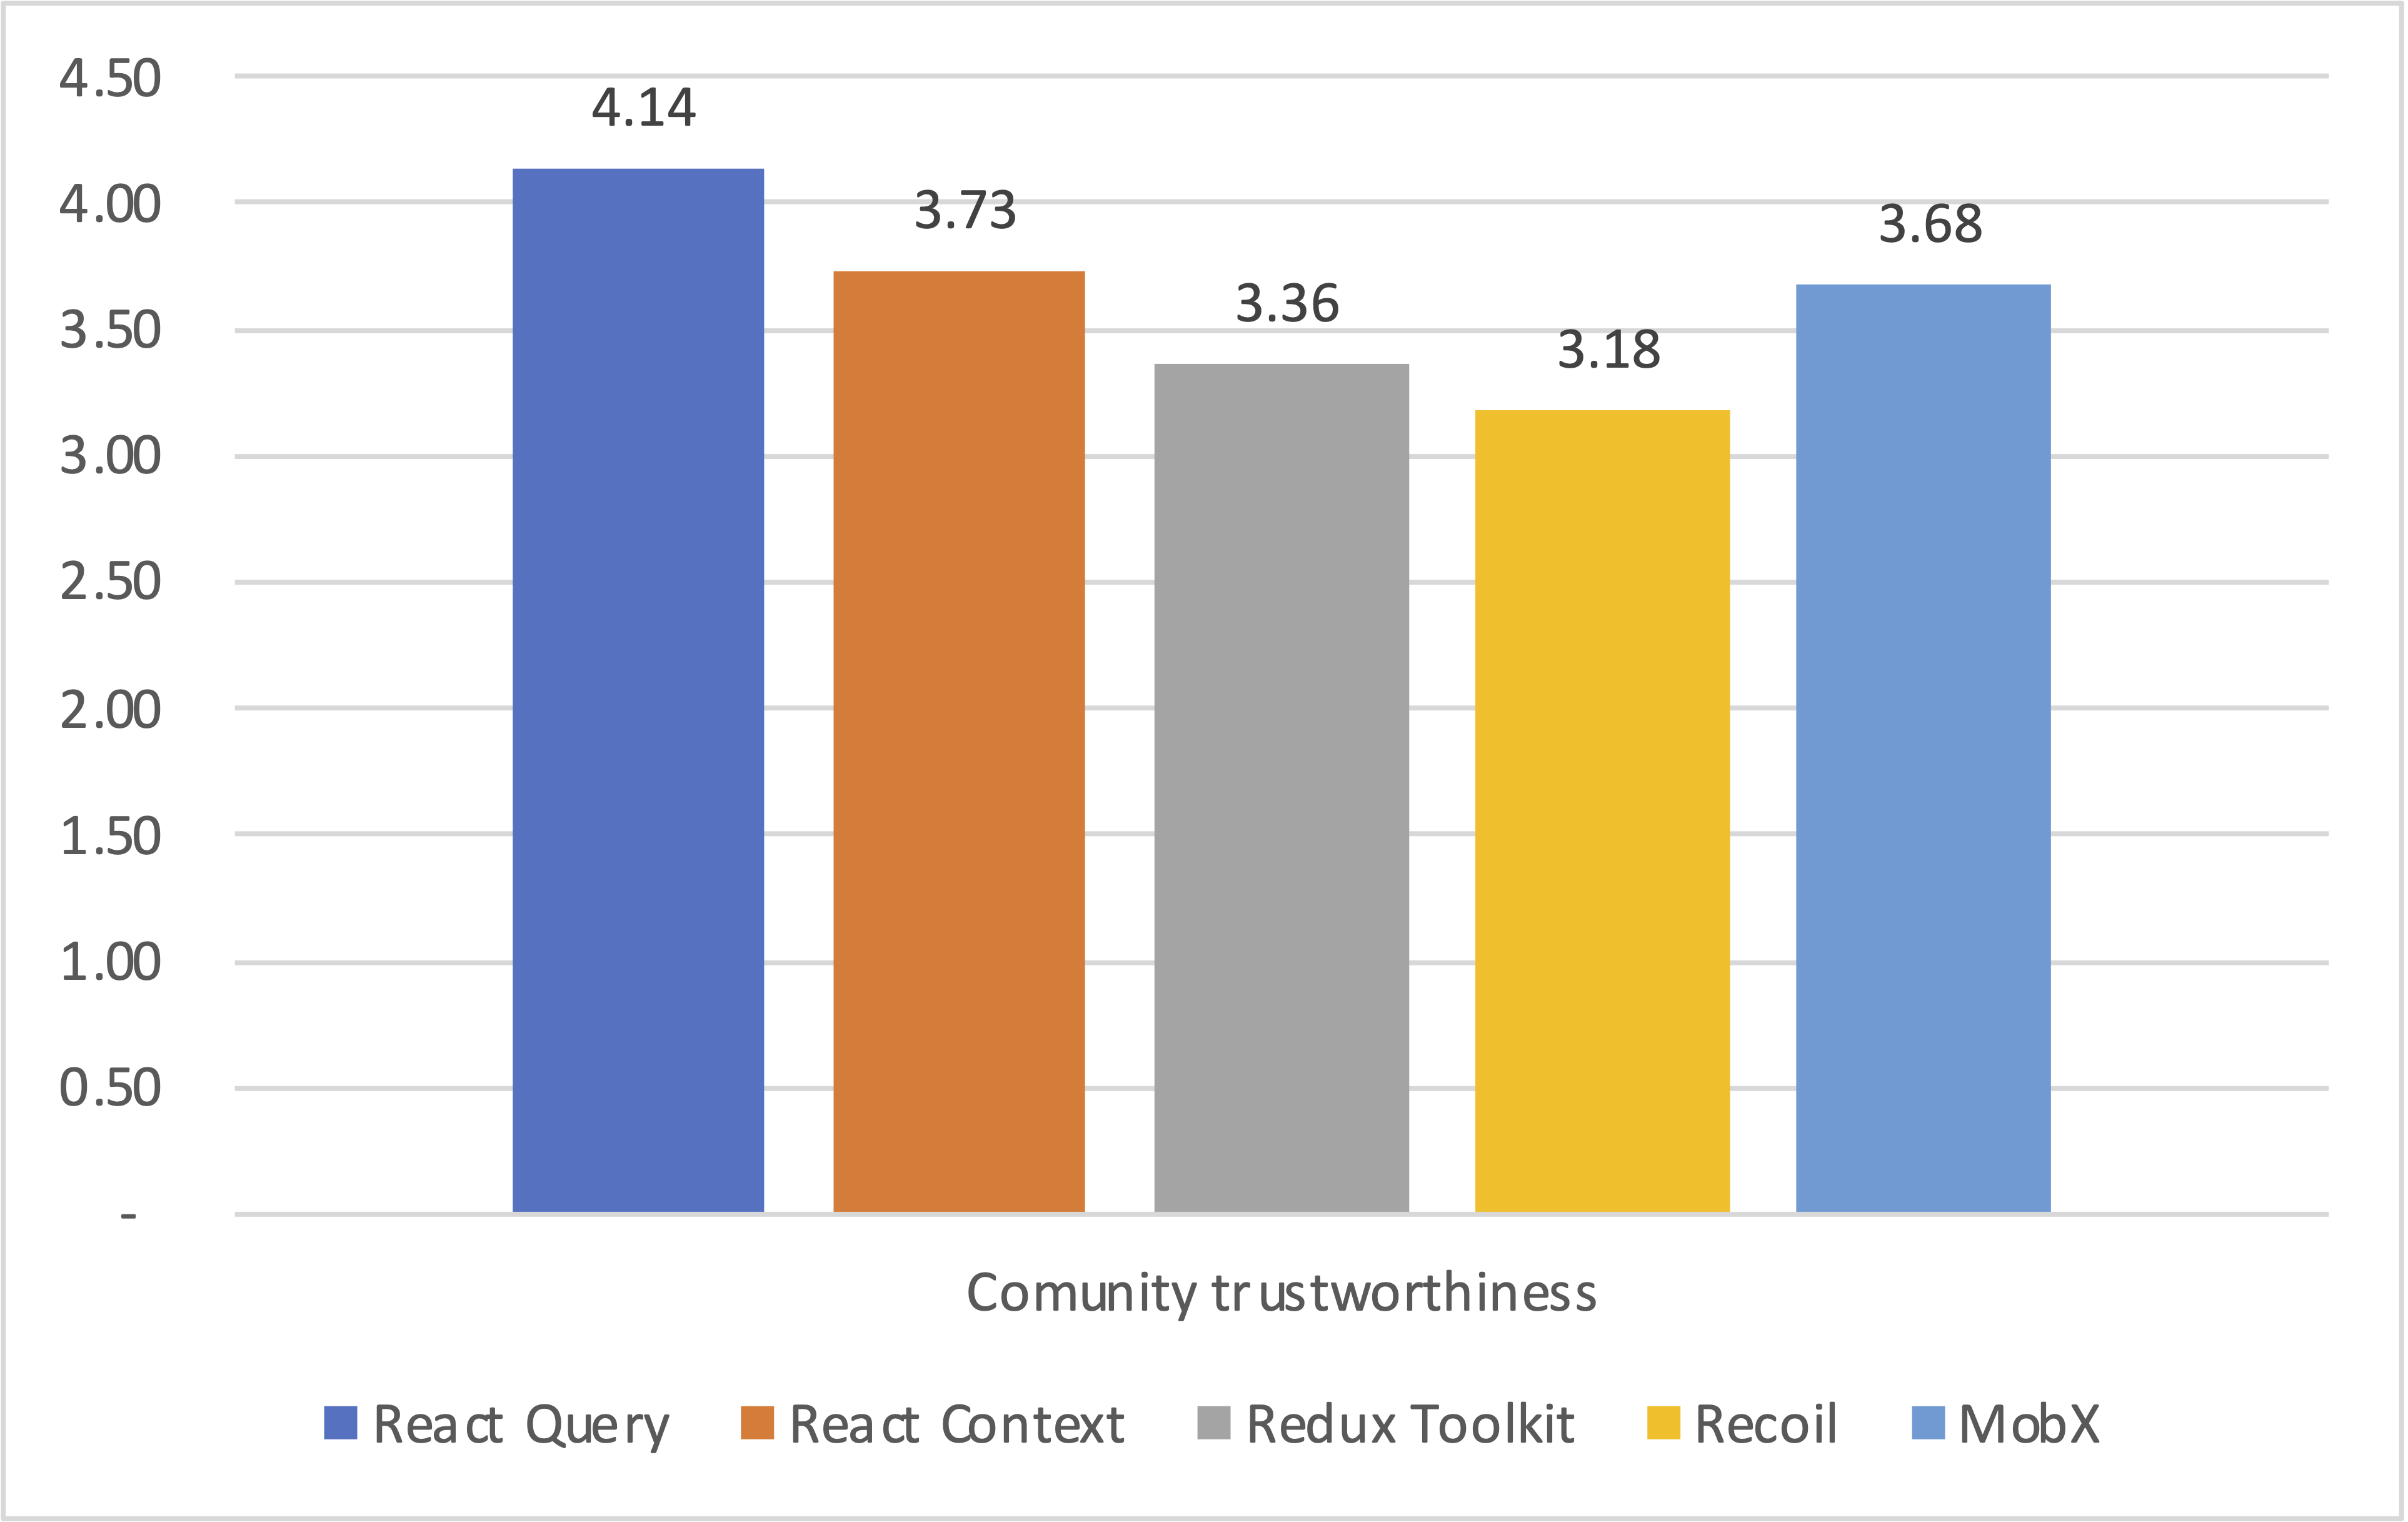
\includegraphics{images/chart_comminity_trustworthiness}
    \caption{Comparison of the community trustworthiness of the five evaluated SMLs}
    \label{image_results_community_trustworthiness}
\end{figure}

The score achieved by the libraries regarding to the second goal,
`Community Trustworthiness' are shown on figure~\ref{image_results_community_trustworthiness},
where a gradual
distribution can be seen. React Query has shown the highest degree of
trustworthiness thanks to the availability of support and consulting
services for sponsors as well as e-learning materials. This is
complemented by the high number of its contributors and an extensive
documentation. On the second and third place come React Context and MobX
with neighboring scores of 3.75 and 3.68 respectively. Redux Toolkit and
Recoil, which occupy the penultimate and last places have a relatively
low number of involved developers and low degree of activity of their
communities. This can be explained in the case of MobX by the high index
of unanswered threads on Stack Overflow and in Recoil by the low number
of threads per year on Stack Overflow.

\hypertarget{product-attractiveness}{%
    \subsection{Product Attractiveness}\label{product-attractiveness}}

\begin{figure}
    \centering
    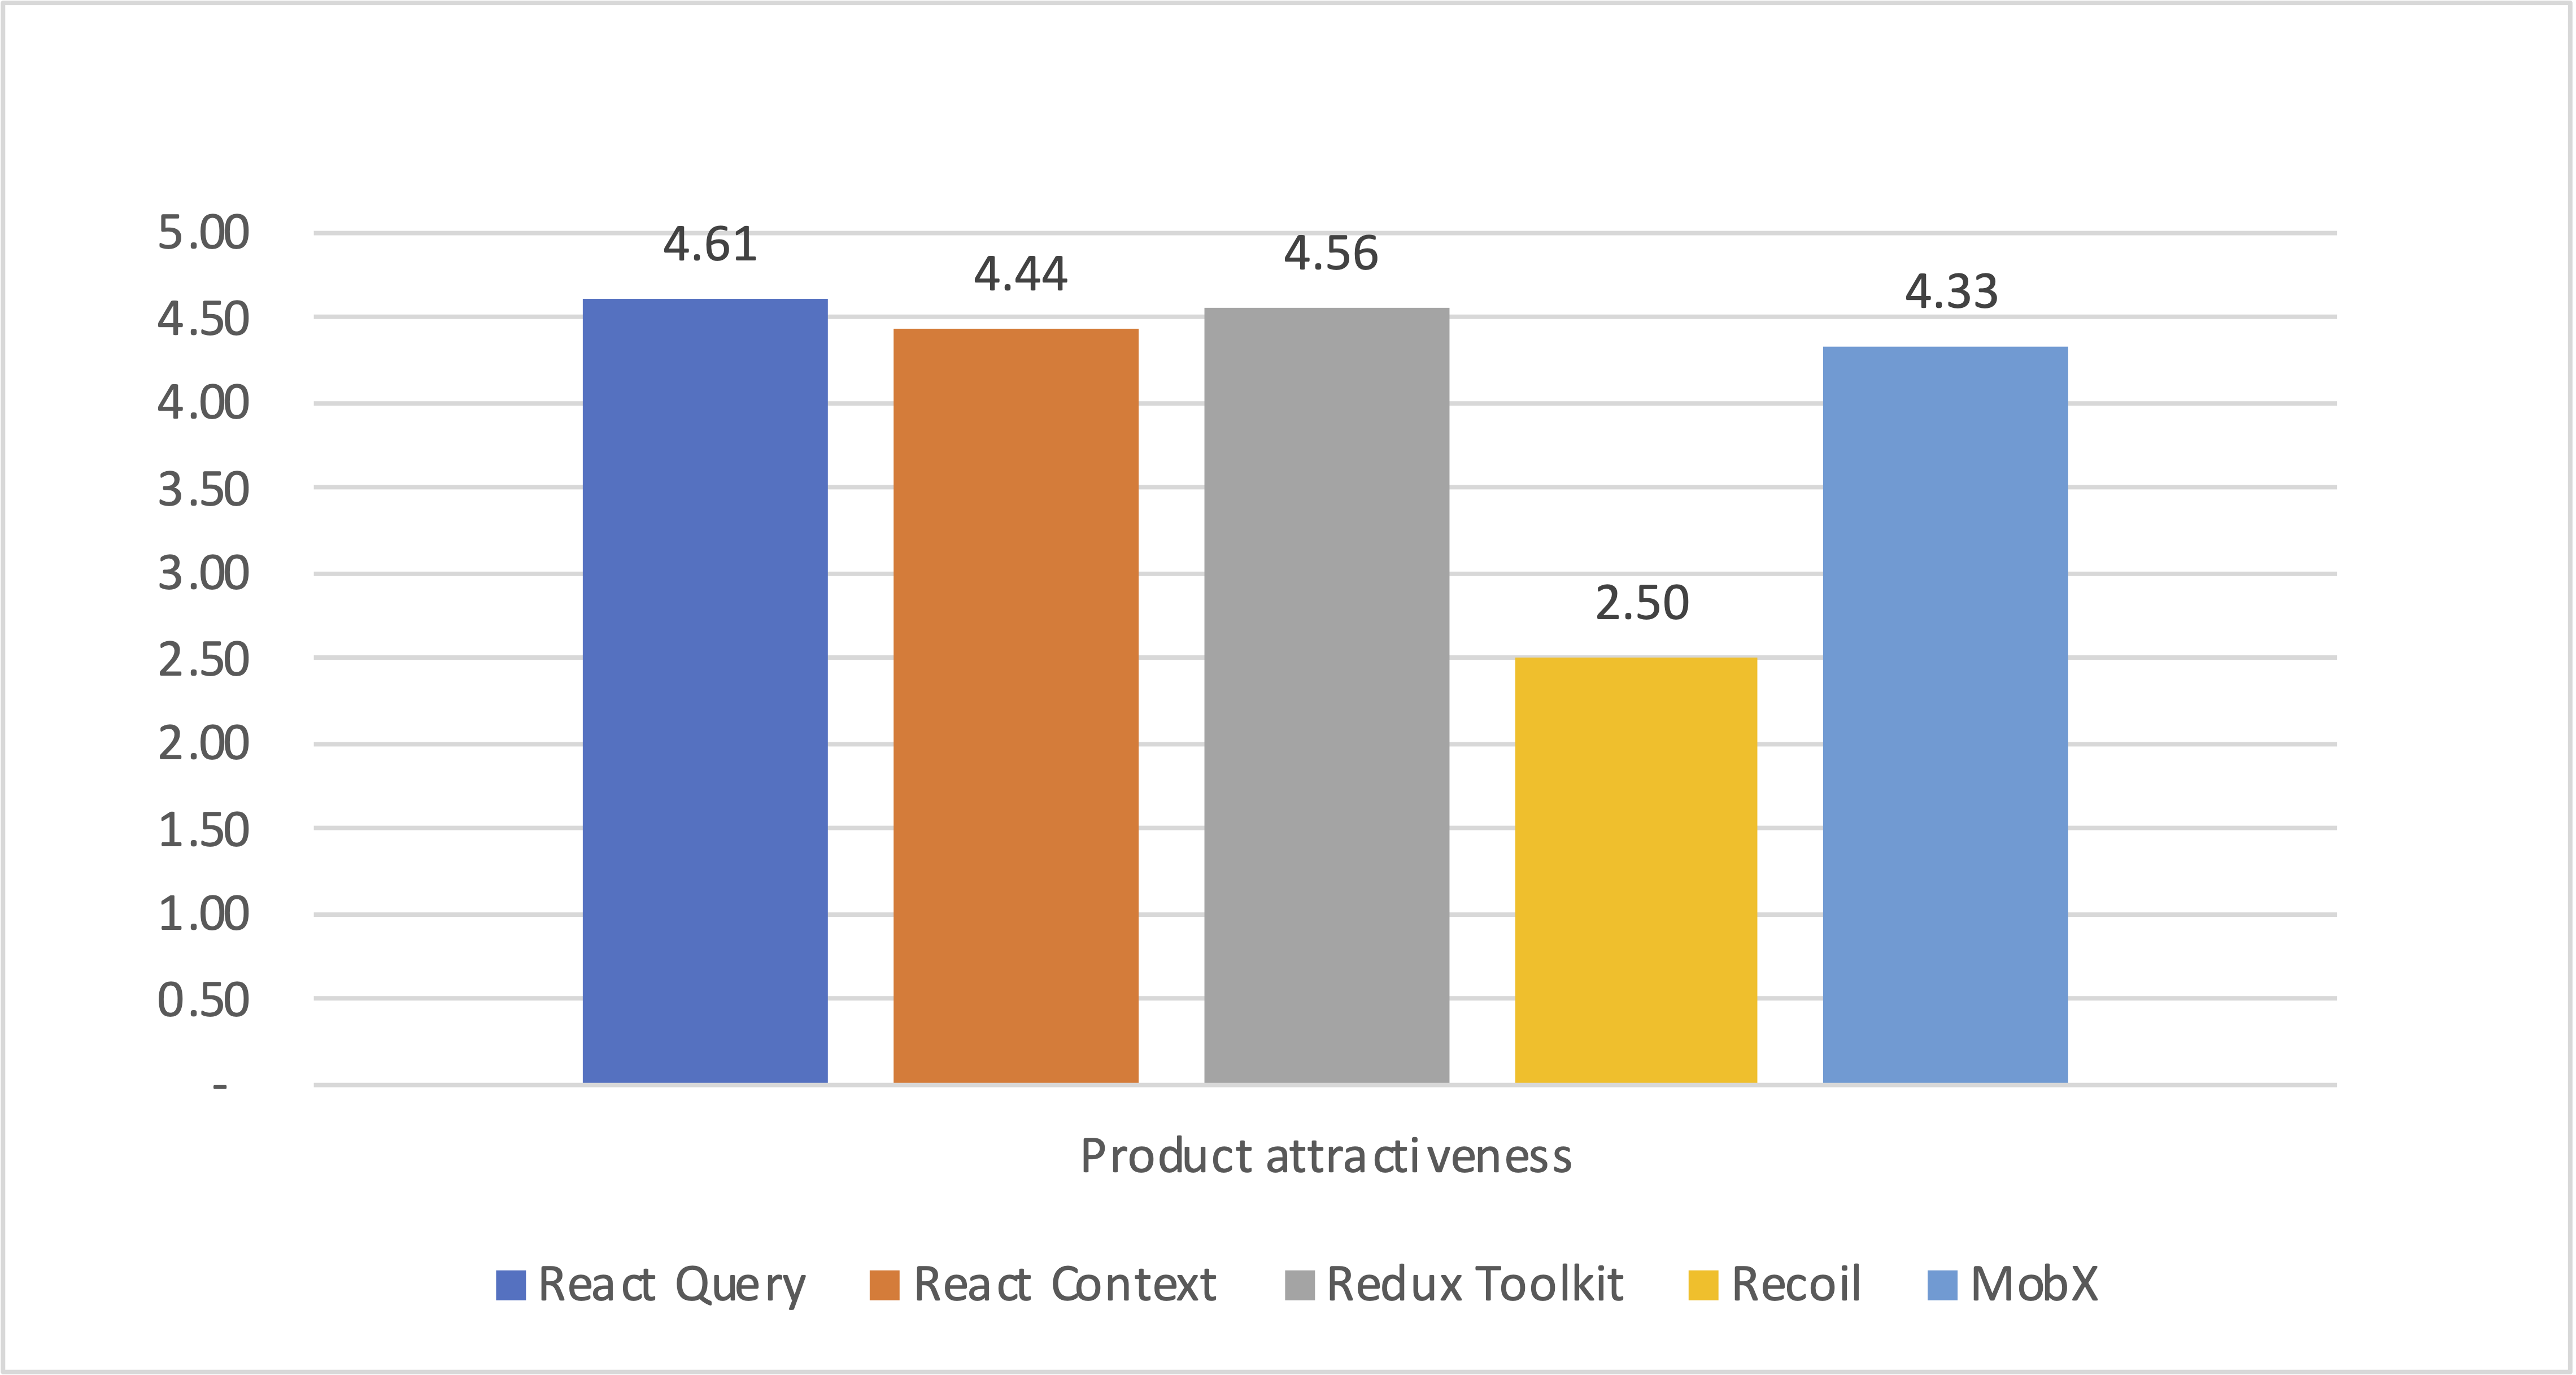
\includegraphics{images/chart_attractiveness}
\caption{Comparison of the product attractiveness of the five evaluated SMLs}
\label{image_results_product_attractiveness}
\end{figure}

The results of the Goal `Product attractiveness' depicted in the figure~\ref{image_results_product_attractiveness} reveal that with the exception of Recoil, the libraries perform at
a similar level. Looking into the questions and metrics that lead to the
score, it can be established that Recoil's low number of weekly
downloads is the main driver. Additionally, the low amount of threads in
Stack Overflow combined with a relatively high number of unanswered
questions contributed in the low score. Interestingly, the project has
more stars and forks on GitHub than Redux Toolkit. This may be explained
by the fact that Recoil is still in an experimental state in the time of
this study and that it is maintained by the same team behind React~\cite{recoil}.

\hypertarget{suitability-the-approaches}{%
    \section{Suitability of the
    Approaches}\label{suitability-the-approaches}}

After the in depth comparison of the state management libraries has been
conducted, the suitability of each library is to be discussed. Thereby
it is important to note that the choice of a technology will most likely
involve other business related factors.

Drawing from the previous results, it has become clear that React
Context is perfectly suitable to handle global state. It is therefore a
good fit for states that are used globally and entail little logic like
the application theme, the currently authenticated user or the selected
locale. Since such a global state usually requires a change
in the whole UI, the re-rendering optimization provided by other
approaches are irrelevant.

React Query has shown that although it can be stretched to manage client
state, it is best suitable for applications whose state lies in a
backend server and needs to be synchronized with the client. Most
notably when server state is shared in multiple parts of the UI, the
built in cache can be utilized to reduce the API calls. It is also best
suitable for improving the user experience by the ease of implementing optimistic
updates. This makes React Query a good solution for building a new user
interface for an existing backend server.

When client side state needs to be shared as well, Redux Toolkit can be
an appropriate choice. Redux Toolkit provides all the tools needed for
creating a software product of high quality, mainly a built in query
client, a concise API, and a high level of testability.

MobX is a minimalistic yet effective library that can be easily learned,
thanks to its use of the OOP paradigm. Since it supports class
components, it can be a good suit for a slow introduction in a legacy
React application that does not use function components. Moreover,
thanks to its simple integration with react, it can be a good solution
to solve one of the presented problems with little
changes in the application.

Lastly, Recoil's strength in defining atoms and explicitly building a
dependency tree to represent an application state hints to its
suitability for complex applications where performance is a requirement,
such as a graphics editor.

\hypertarget{hypotheses-verification}{%
    \section{Hypotheses Verification}\label{hypotheses-verification}}

After defining the suitability of the application of the libraries, the
hypotheses presented in chapter~\ref{motivation-and-hypotheses} can be verified
on the basis of the performed analysis.

This study confirms the first hypothesis: ``React Context is
best suited for data which is rarely changed, such as the authenticated
user or the current UI theme.'' As previously stated, React Context
solves the problem of prop drilling and therefore is suitable for the
above mentioned use case.

The second hypothesis: ``State Management Libraries are suitable for
complex User Interfaces (UIs) that don't communicate much with a backend
server.'' can only be partially confirmed when the term State Management
Libraries is interpreted as MobX, Recoil and Redux Toolkit. As explained
in the previous chapter, these libraries do support complex client
states, but there is no restriction when it comes to communicating with
a backend server since API calls can be made within all of them.
Additionally Redux Toolkit also offers the functionality to communicate
with a backend server through its built-in query client~\cite{rtk_query}.

The third hypothesis: ``Query approaches are better suited for UIs, that
need to interact with a backend server.'' is also confirmed. As
previously presented, React Query fulfills the requirements of
communicating with a backend server, by managing API calls, cache,
loading states and optimistic updates.

\hypertarget{reflection}{%
    \section{Reflection}\label{reflection}}

Before concluding this thesis, it is important to reflect on the
research process. This includes remarks and takeaways that emerged
during the practical application of the research design. These are
related to the usage of metrics and the application of the framework
EFFORT\@.

\hypertarget{usage-of-metrics}{%
    \subsection{Usage of Metrics}\label{usage-of-metrics}}

The use of metrics in the scope of this thesis was implicitly assumed,
yet their practical usage comes with various challenges. The first
challenge lies in the interpretation of the metrics. For example `The
average threads per year in Stack Overflow' can be interpreted
differently. A low value could mean a low adoption of the product or
that it has reached a stable state and its usage is clear. A better
metric could analyze the evolution of the tread count in Stack Overflow
to verify the stability and maturity of the product. A similar effect
can be seen in the metric `The number of major releases per year'. Other
metrics were arguably less practical. These include ``the Average number
of commits per committer'', whose goal is to determine the level of
commitment the maintainers have. The result could be easily diluted: A
lower number could be justified by the core maintainers actively
promoting maintaining the project. An alternative metric that would
fulfill the same goal could be `Count of authors who have 50 commits or
more'. Yet, new metrics need to be tested in order to avoid similar
problems and edge cases.

Another challenge emerges from the fact that knowing about the usage of
metrics had a clear impact on the produced code. For instance, being
aware of the metric ``code duplication'', has led to a perfect
measurement of 0 in the applications of all the libraries. A more
practical indicator could be for example `The tendency of developers to
write repetitive code when using the library', which could be measured
by analyzing open source projects that use the library. This leads to a
broader topic concerning the effect of metrics on the developers. Or as
Goodhart's law (named after British economist Charles Goodhart) puts it: ``When a measure becomes a target, it ceases
to be a good measure''~\cite{goodhart}.
The usage of quantitative metrics has also shown little
usefulness. Namely the application of the metric ``Cognitive
complexity'' in the context of the thesis experiments has proven to be
incomplete for the reason that it does not consider the knowledge of
third party libraries required to understand the code. Ideally this
metric would include the degree to which the library is incorporated
into the source code. Other qualitative metrics has yielded very similar
results, such as the `Count of Lines of Code', `Count of functions' and
`Count of statements'. Moreover, multiple metrics are defined
specifically for OOP languages. This may explain the limited choice of
static code analysis tools available for the used programming language
(TypeScript) in comparison to other programming languages, such as
Java. It is to mention, that although the used language does support the
OOP paradigms such as class definitions, interfaces and inheritance, it
is seldom used in that way. Generally, there seems to be a gap between
metrics proposed in scientific papers, which have a sound and
mathematical basis and the one that can be measured in practice.

All in all, the results point out that qualitative metrics play a bigger
role when choosing a software product. This introduces a level of
subjectivity into the assessment process, which is understandable since
the choice of a software product is influenced by other factors and
needs to fulfill greater requirements than the technical aspects.
Luckily, the flexibility of EFFORT provided by the instantiation step
allows for great customization to match user specific use cases.

\hypertarget{effort-1}{%
    \subsection{EFFORT}\label{effort-1}}

The possibility to edit and add goals, questions, and
metrics within EFFORT is an advantage over many of the other
approaches. The practicability of the framework comes from the
definition of metric mappings that brings the values to the same range
of 1-5, from the possibility to define a positive or negative metric,
the relevance of the questions, and finally from having a formula to
calculate the performance within goal. Yet there have been a few
ambiguities during the application. For one, the mapping values defined
as (1 = inadequate, 2 = poor, 3 = sufficient, 4 = good, and 5 =
excellent) can be misleading, since each metric can have either a
positive or negative interpretation. A scale from lowest to highest
would be more clear for the user.

Moreover, the framework doesn't explicitly allow the removal of the
baseline version questions, goals or metrics that are not applicable to
the application domain. This was deduced from the example application on
ERP systems where the sub-goal ``Security'' was left out~\cite{effort}.

Other ambivalences were experienced, such as the term ``Technology
concentration'' used under the maintainability goal, as well as the
absence of the source of the metrics and how to measure them, and
the differentiation between question markers in
the FlOSS context and in the specific context \cite{effort}.
Additionally no instructions are given on creating the metric mappings.
In the carried out experiments, the quantitative metric mappings were
created after the raw metric results were collected. Although the
metrics may be general, this results in a use case specific mapping.
Plus, the mapping of the metrics as a whole depends greatly on the
selected software products to be compared.

All things considered, the adoption of the framework EFFORT for the
comparison has yielded satisfying results. Its high level of
customizability has allowed the comparison of libraries, although it was
previously only used to compare standalone applications.

\hypertarget{conclusion-and-future-work}{%
    \chapter{Outro}\label{conclusion-and-future-work}}

This work has given an in depth analysis of state management libraries
and provided general conclusions about the suitability of each approach.
By using the EFFORT framework, a found comparison based on software quality
characteristics could be made. Since only a selection of libraries was analyzed,
future work could include other libraries by using the proposed instantiation of EFFORT,
especially to compare state management libraries within the same category.
Related topics, which were out of the scope of this study, could be the subject
of further research projects. Among others, further research could address
ambiguities related to the interpretation of metrics by extending the existing
qualitative and quantitative metrics for open source software and providing
standard metric values in order to facilitate the creation of metric mappings.



%% appendix if used
%%\appendix
\typeout{===== File: appendix}

\begin{appendices}
\chapter{EFFORT Instantiation}\label{appendix_a_effort_instantiation}

%%\setlength\tabcolsep{2pt}
%\caption{My caption}
%\label{lbl}
\begin{tabular}[]{|p{1cm}p{2cm}p{1.5cm}p{1.5cm}p{5cm}p{2.5cm}|}

Q-Id & Question & Q-State & M-Id & Metric & M-state \\
\hline
    \hline
1a.1 & Adaptability & KEPT & 1a.1.1 & Number of operating systems
supported & REMOVED \\
& & & 1a.1.2 & Support for Function and Class Components & ADDED \\
& & & 1a.1.3 & Adoption of React Suspense & ADDED \\
1a.2 & Installability & KEPT & 1a.2.1 & Time required for installation &
REMOVED \\
& & & 1a.2.2 & Availability of the installation manual & KEPT \\
& & & 1a.2.3 & Automation level and use of installation scripts &
REMOVED \\
& & & 1a.2.4 & Dependence on third-party components & KEPT \\
& & & 1a.2.5 & Nominal length of the installation procedures &
REMOVED \\
& & & 1a.2.6 & Number of configuration files Minimum number of files
added and changed for minimum functionality & CHANGED \\
& & & 1a.2.7 & Availability and rationality of default options &
CHANGED \\
& & & 1a.2.8 & Internationalisation of the manual & KEPT \\
& & & 1a.2.9 & Number of unforeseen issues & KEPT \\
& & & 1a.2.10 & Degree of knowledge of the required operating
environment & KEPT \\
& & & 1a.2.11 & Efficacy of the guide & KEPT \\
1a.3 & Replaceability & KEPT & 1a.3.1 & Existence of other libraries
with the same functionality and a similar API & ADDED \\
1a.4 & Coexistence & REMOVED & & & \\
\end{tabular}

%\begin{longtable}[]{@{}llllllll@{}}
\toprule
GoalId & Goal & QuestionId & Question & QuestionState & MetricId &
Metric & Metric state \\
\midrule
\endhead
1a & Portability & 1a.1 & Adaptability & KEPT & 1a.1.1 & Number of
operating systems supported & REMOVED \\
& & & & & 1a.1.2 & Support for Function and Class Components & ADDED \\
& & & & & 1a.1.3 & Adoption of React Suspense & ADDED \\
& & 1a.2 & Installability & KEPT & 1a.2.1 & Time required for
installation & REMOVED \\
& & & & & 1a.2.2 & Availability of the installation manual & KEPT \\
& & & & & 1a.2.3 & Automation level and use of installation scripts &
REMOVED \\
& & & & & 1a.2.4 & Dependence on third-party components & KEPT \\
& & & & & 1a.2.5 & Nominal length of the installation procedures &
REMOVED \\
& & & & & 1a.2.6 & Number of configuration files Minimum number of files
added and changed for minimum functionality & CHANGED \\
& & & & & 1a.2.7 & Availability and rationality of default options &
CHANGED \\
& & & & & 1a.2.8 & Internationalisation of the manual & KEPT \\
& & & & & 1a.2.9 & Number of unforeseen issues & KEPT \\
& & & & & 1a.2.10 & Degree of knowledge of the required operating
environment & KEPT \\
& & & & & 1a.2.11 & Efficacy of the guide & KEPT \\
& & 1a.3 & Replaceability & KEPT & 1a.3.1 & Existence of other libraries
with the same functionality and a similar API & ADDED \\
& & 1a.4 & Coexistence & REMOVED & & & \\
1b & Maintainability & 1b.1 & Analyzability & KEPT & 1b.1.1 &
Availability and quality of developer tools & ADDED \\
& & 1b.2 & Changeability & REMOVED & & // because libraries cannot be
changed by definition & \\
& & 1b.3 & Testability & KEPT & 1b.3.1 & Possibility to test business
logic without React & ADDED \\
& & 1b.4 & Technology concentration & REMOVED & & // ambiguous term:
"Technology concentration" & \\
& & 1b.5 & Stability & KEPT & 1b.5.1 & Breaking API changes & ADDED \\
& & 1b.6 & How maintainable is the application code using the product? &
ADDED & 1b.6.1 & Code duplication & ADDED \\
& & & & & 1b.6.2 & Cyclomatic complexity & ADDED \\
& & & & & 1b.6.3 & Cognitive complexity & ADDED \\
\bottomrule
\end{longtable}

%\begin{longtable}[]{@{}llllllll@{}}
\toprule
GoalId & Goal & QuestionId & Question & QuestionState & MetricId &
Metric & Metric state \\
\midrule
\endhead
1c & Reliability & 1c.1 & Rebustness & REMOVED & & // non applicable to
domain & \\
& & 1c.2 & Recoverability & REMOVED & & // non applicable to domain & \\
1d & Functionallity & 1d.1 & Functional adequacy & KEPT & 1d.1.1 &
Possibility to share state without prop drilling. & ADDED \\
& & & & & 1d.1.2 & Possibility to have derived state. & ADDED \\
& & 1d.2 & Interoperability & KEPT & 1d.2.1 & Level of data
importability & REMOVED \\
& & & & & 1d.2.2 & Level of data exportability & REMOVED \\
& & & & & 1d.2.3 & Availability of community plugins & ADDED \\
& & 1d.3 & Functional accuracy & KEPT & 1d.3.1 & Lines of code &
ADDED \\
& & & & & 1d.3.2 & Statement count & ADDED \\
& & & & & 1d.3.3 & Functions count & ADDED \\
1e & Usability & 1e.1 & Pleasantness & REMOVED & & // non applicable to
domain & \\
& & 1e.2 & Operability & KEPT & 1e.2.1 & Availability and quality of
developer tools (same as 1b.1.1) & ADDED \\
& & 1e.3 & Understandability & REMOVED & & // non applicable to domain
& \\
& & 1e.4 & Learnability & KEPT & - & Same metrics as in Question 2.5 &
ADDED \\
1f & Efficiency & 1f.1 & Time behavior & KEPT & 1f.1.1 & First
Contentful Paint & ADDED \\
& & & & & 1f.1.2 & Speed Index & ADDED \\
& & & & & 1f.1.3 & Largest Contentful Paint & ADDED \\
& & & & & 1f.1.4 & Time to Interactive & ADDED \\
& & & & & 1f.1.5 & Total Blocking Time & ADDED \\
& & & & & 1f.1.6 & Cumulative Layout Shift & ADDED \\
& & 1f.2 & Resources utilization & KEPT & 1f.2.1 & Efficient re-renders
& ADDED \\
\bottomrule
\end{longtable}

%\begin{longtable}[]{@{}llllll@{}}
\toprule
QuestionId & Question & QuestionState & MetricId & Metric & Metric
state \\
\midrule
\endhead
2.1 & How many developers does the community involve? & KEPT & 2.1.1 &
Number of committers & KEPT \\
2.2 & What degree of activity does the community have? & KEPT & 2.2.1 &
Number of major releases per year & REMOVED \\
& & & 2.2.2 & Average number of commits per year & KEPT \\
& & & 2.2.3 & Average number of commits per committer & KEPT \\
& & & 2.2.4 & Closed bugs index issues on GitHub & CHANGED \\
& & & 2.2.5 & Index of satisfied requests merged pull requests on GitHub
& CHANGED \\
2.3 & Are the support tools available and effective? & KEPT & 2.3.1 &
Average number of threads per year on StackOverflow & KEPT \\
& & & 2.3.2 & Index of unanswered threads on StackOverflow & KEPT \\
& & & 2.3.3 & Number of forums & REMOVED \\
& & & 2.3.4 & Average number of threads per forum & REMOVED \\
& & & 2.3.5 & Average number of posts per year & REMOVED \\
& & & 2.3.6 & Forum internationalisation level & REMOVED \\
& & & 2.3.7 & Number of trackers & REMOVED \\
& & & 2.3.8 & Volume of Wikis Usability of the documentation (same as
2.5.6) & CHANGED \\
& & & 2.3.9 & Number of faqs in the documentation & CHANGED \\
2.4 & Are support services provided? & KEPT & 2.4.1 & Availability of
training services & KEPT \\
& & & 2.4.2 & Temporal coverage of training services & REMOVED \\
& & & 2.4.3 & Availability of e-learning services & REMOVED \\
& & & 2.4.4 & Availability of phone assistance & REMOVED \\
& & & 2.4.5 & Availability of certification services & KEPT \\
& & & 2.4.6 & Availability of outsourcing services & REMOVED \\
& & & 2.4.7 & Availability of maintenance services & REMOVED \\
& & & 2.4.8 & Availability of information and services for TCO
estimation & REMOVED \\
& & & 2.4.9 & Availability of consulting services & KEPT \\
2.5 & Is the documentation exhaustive and easily consultable? & KEPT &
2.5.1 & Number of topics covered in the administrator documentation &
REMOVED \\
& & & 2.5.2 & Number of topics covered in the user documentation &
REMOVED \\
& & & 2.5.3 & Number of topics covered in the technical documentation &
REMOVED \\
& & & 2.5.4 & Number of topics covered in the other documents &
REMOVED \\
& & & 2.5.5 & Number of additional documentation files & REMOVED \\
& & & 2.5.6 & Usability of the documentation & KEPT \\
\bottomrule
\end{longtable}

%\begin{longtable}[]{@{}llllll@{}}
\toprule
QuestionId & Question & QuestionState & MetricId & Metric & Metric
state \\
\midrule
\endhead
3.1 & What degree of functional adequacy does the product offer? & KEPT
& & // Same as 1d.1 & \\
& & & 3.2.1 & Number of weekly downloads & CHANGED \\
3.2 & What degree of diffusion does the product achieve? & KEPT & 3.2.2
& Freshmeat popularity index Number of stars on GitHub & CHANGED \\
& & & 3.2.3 & Number of rating source forge users Number of forks on
GitHub & CHANGED \\
& & & 3.2.4 & Positive rating index & REMOVED \\
& & & 3.2.5 & Number of success stories & REMOVED \\
& & & 3.2.6 & Google visibility & REMOVED \\
& & & 3.2.7 & Number of official partners/spronsors & CHANGED \\
& & & 3.2.8 & Number of published books & KEPT \\
& & & 3.2.9 & Number of citations by domain expert & REMOVED \\
& & & 3.2.10 & Number State of academic publications & CHANGED \\
& & & 3.2.11 & Sponsor availability & KEPT \\
3.3 & What level of cost-effectiveness is estimated? & REMOVED & 3.3.1 &
Availability of services and information for the estimation of the TCO &
REMOVED \\
& & & 3.3.2 & Availability of an edition without license cost &
REMOVED \\
& & & 3.3.3 & Cost of the minimal edition & REMOVED \\
& & & 3.3.4 & Cost of the complete edition & REMOVED \\
3.4 & What degree of reusability and redistribution is left by the
license? & KEPT & 3.4.1 & License type & KEPT \\
\bottomrule
\end{longtable}


\section{Questions Definition}

Table \ref{table:questions_minified} displays the
questions defined during the instantiation of EFFORT
along with their relevance within their associated goals.
$*$ means the question has been added,
$^{\square}$ means the question has not been changed, and
$^{\times}$ means the question has been removed.

\begin{longtable}[]{|p{1cm}p{10cm}p{2cm}|}
    \caption{Questions defined during the instantiation of EFFORT.}
    \label{table:questions_minified}\\
    \toprule
Id & Question & Relevance \\
\midrule
\endhead
1a.1 & What degree of Adaptability does the product offer?$^{\square}$ & 2 \\
1a.2 & What degree of Installability does the product offer?$^{\square}$ & 1 \\
1a.3 & What degree of Replaceability does the product offer?$^{\square}$ & 2 \\
1a.4 & What degree of Coexistence does the product offer?$^{\times}$ & \\
1b.1 & What degree of Analyzability does the product offer?$^{\square}$ & 2 \\
1b.2 & What degree of Changeability does the product offer?$^{\times}$ & \\
1b.3 & What degree of Testability does the product offer?$^{\square}$ & 2 \\
1b.4 & What degree of Technology concentration does the product offer?$^{\times}$ & \\
1b.5 & What degree of Stability does the product offer?$^{\square}$ & 2 \\
1b.6 & How maintainable is the application code using the product?* & 2 \\
1c.1 & What degree of Rebustness does the product offer?$^{\times}$ & \\
1c.2 & What degree of Recoverability does the product offer?$^{\times}$ & \\
1d.1 & What degree of Functional adequacy does the product offer?$^{\square}$ & 3 \\
1d.2 & What degree of Interoperability does the product offer?$^{\square}$ & 2 \\
1d.3 & What degree of Functional accuracy does the product offer?$^{\square}$ & 2 \\
1e.1 & What degree of Pleasantness does the product offer?$^{\times}$ & \\
1e.2 & What degree of Operability does the product offer?$^{\square}$ & 1 \\
1e.3 & What degree of Understandability does the product offer?$^{\times}$ & \\
1e.4 & What degree of Learnability does the product offer?$^{\square}$ & 2 \\
1f.1 & What degree of Time behavior does the product offer?$^{\square}$ & 2 \\
1f.2 & What degree of Resources utilization does the product offer?$^{\square}$ & 3 \\
2.1 & How many developers does the community involve?$^{\square}$ & 3 \\
2.2 & What degree of activity does the community have?$^{\square}$ & 2 \\
2.3 & Are the support tools available and effective?$^{\square}$ & 2 \\
2.4 & Are support services provided?$^{\square}$ & 1 \\
2.5 & Is the documentation exhaustive and easily consultable?$^{\square}$ & 3 \\
3.1 & What degree of functional adequacy does the product offer?$^{\square}$ & 3 \\
3.2 & What degree of diffusion does the product achieve?$^{\square}$ & 2 \\
3.3 & What level of cost-effectiveness is estimated?$^{\times}$ & \\
3.4 & What degree of reusability and redistribution is left by the
license?$^{\square}$ & 1 \\
\bottomrule
\end{longtable}


\section{Metrics Definition}

Table \ref{table:metrics_minified} displays the
metrics defined during the instantiation of EFFORT, where
$*$ means the metric has been added,
$^{\Delta}$ means the metric has been changed,
$^{\square}$ means the metric has not been changed, and
$^{\times}$ means the metric has been removed.
Additionally, negatively interpreted metrics are marked with $(-)$
and positive ones with $(+)$.

\begin{longtable}[]{|p{1cm}p{6cm}p{6cm}|}
    \caption{Metrics defined during the instantiation of EFFORT.}
    \label{table:metrics_minified}\\
\toprule
Id & Metric & Metric mapping \\
\midrule
\endhead
1a.1.1 & Number of operating systems supported$^{\times}$ & \\
1a.1.2 & Support for Function and Class Components*$(+)$ & No=1 Yes=5 \\
1a.1.3 & Adoption of React Suspense*$(+)$ & Implementation available=5
Planned=3 No=1 \\
1a.2.1 & Time required for installation$^{\times}$ & \\
1a.2.2 & Availability of the installation manual$^{\square}(+)$ & No=1 Yes=5 \\
1a.2.3 & Automation level and use of installation scripts$^{\times}$ & \\
1a.2.4 & Dependence on third-party components$^{\square}(-)$ & 0=1 1-5=2 5-10=3 10-15=4 15-20=5 \\
1a.2.5 & Nominal length of the installation procedures$^{\times}$ & \\
1a.2.6 & Minimum number of files added and changed for minimum functionality$^{\Delta}(-)$ & One file=1 Two files = 3 Three and higher=5 \\
1a.2.7 & Availability and rationality of default options$^{\Delta}(+)$ & No default options=1 Default options provided=3 Useful/rational default options provided=5 \\
1a.2.8 & Internationalisation of the manual$^{\square}(+)$ & Multiple languages supported=5 English supported=3 Only non-english language supported=1 \\
1a.2.9 & Number of unforeseen issues$^{\square}(-)$ & Zeo issues=1 Two/Three issues=3 More issues=5 \\
1a.2.10 & Degree of knowledge of the required operating environment$^{\square}(-)$ & Little previous knowledge required=1 Medium knowledge required=3 Understanding of a paradigm required=5 \\
1a.2.11 & Efficacy of the guide$^{\square}(+)$ & Installation guide non existing=1
Installation guide available=5 \\
1a.3.1 & Existence of other libraries with the same functionality and a
similar API*$(+)$ & No equivalent library available=1 \textless{} 3 Similar
libraries available=3 3+ similar libraries available=5 \\
& & \\
1b.1.1 & Availability and quality of developer tools*$(+)$ & No=1 Yes=3 Yes,
with advanced debugging features=5 \\
1b.3.1 & Possibility to test business logic without React*$(+)$ & No=1 Yes=5 \\
1b.5.1 & Breaking API changes*$(+)$ & Breaking API changes in major versions=1
Breaking API changes in major versions with migrations guide=3 Breaking
API changes in major versions with migration guide and codemod=4 No
breaking API changes introduced major update=5 \\
1b.6.1 & Code duplication*$(-)$ & 0=1 1-10=2 10-20=3 10-30=4 30+=5 \\
1b.6.2 & Cyclomatic complexity*$(-)$ & 0-92=1(Base 82) 92-102=2 102-112=3 112-122=4 122+=5 \\
1b.6.3 & Cognitive complexity*$(-)$ & 1-10=1 11-20=2 21-50=4 Over 50=5 \\
1d.1.1 & Possibility to share state without prop drilling*$(+)$ & No=1 Yes=5 \\
1d.1.2 & Possibility to have derived state*$(+)$ & No=1 Yes, through React=3 Yes=5 \\
1d.2.1 & Level of data importability$^{\times}$ & \\
1d.2.2 & Level of data exportability$^{\times}$ & \\
1d.2.3 & Availability of community plugins*$(+)$ & No=1 Yes=5 \\
1d.3.1 & Lines of code*$(-)$ & 0-685=1 685-710=2 710-735=3 735-760=4 760+=5 \\
1d.3.2 & Statement count*$(-)$ & 0-114=1 114-124=2 124-144=3 134-144=4 Over
144=5 \\
1d.3.3 & Functions count*$(-)$ & 0-59=1 59-69=2 69-79=3 79-89=4 Over 89=5 \\
& // non applicable to domain & \\
1e.2.1 & Availability and quality of developer tools*$(+)$ (same as 1b.1.1) &
No=1 Yes=3 Yes, with advanced debugging features=5 \\
& // non applicable to domain & \\
- & Same metrics as in Question 2.5 & - \\
1f.1.1 & First Contentful Paint*$(-)$ & 0-1.8=1 1.8-3=3 Over 3=5 \\
1f.1.2 & Speed Index*$(-)$ & 0--3.4=1 3.4--5.8=3 Over 5.8=5 \\
1f.1.3 & Largest Contentful Paint*$(-)$ & 0--2.5=1 2.5--4=3 Over 4=5 \\
1f.1.4 & Time to Interactive*$(-)$ & 0--3.8=1 3.8--7.3=3 Over 7.3=5 \\
1f.1.5 & Total Blocking Time*$(-)$ & 0--200=1 200--600=3 Over 600=5 \\
1f.1.6 & Cumulative Layout Shift*$(-)$ & 0--0.1=1 0.1--0.25=3 Over 0.25=5 \\
1f.2.1 & Efficient re-renders*$(+)$ & Redundant re-renders=1 Suboptimal
re-renders=3 Optimal re-renders=5 \\
2.1.1 & Number of committers$^{\square}(+)$ & 0-100=1 100-200=2 200-300=3 300-400=4
Over 400=5 \\
2.2.1 & Number of major releases per year$^{\times}$ & \\
2.2.2 & Average number of commits per year$^{\square}(+)$ & 0=1 1-10=2 10-100=3
100-1000=4 Over 1000=5 \\
2.2.3 & Average number of commits per committer$^{\square}(+)$ & 0-2.5=1 2.5-5=2
5-7.5=3 7.5-10=4 Over 10=5 \\
2.2.4 & Closed issues on GitHub$^{\Delta}(+)$ & 0-250=1 250-500=2 500-750=3
750-1000=4 Over 1000=5 \\
2.2.5 & Index of merged pull requests on GitHub$^{\Delta}(+)$ &
0-250=1 250-500=2 500-750=3 750-1000=4 Over 1000=5 \\
2.3.1 & Average number of threads per year on Stack Overflow$^{\Delta}(+)$ & 0-200=1
200-400=2 400-600=3 600-800=4 Over 800=5 \\
2.3.2 & Index of unanswered threads on Stack Overflow$^{\Delta}(-)$ & 0-5=1 5-10=2
10-15=3 15-20=4 Over 20=5 \\
2.3.3 & Number of forums$^{\times}$ & \\
2.3.4 & Average number of threads per forum$^{\times}$ & \\
2.3.5 & Average number of posts per year$^{\times}$ & \\
2.3.6 & Forum internationalisation level$^{\times}$ & \\
2.3.7 & Number of trackers$^{\times}$ & \\
2.3.8 & Usability of the documentation (same as 2.5.6)$^{\Delta}(+)$ &
Documentation provides no instructions=1 Documentation includes
installation instructions=2 Documentation provides project setup=3
Documentation provides hello world=4 Documentation provides advanced
examples and guides=5 \\
2.3.9 & Number of faqs in the documentation$^{\Delta}(+)$ & No FAQ available=5
\textless{} 10 Questions=3 11+ Questions=5 \\
2.4.1 & Availability of training services$^{\square}(+)$ & No=1 Yes=5 \\
2.4.2 & Temporal coverage of training services$^{\times}$ & \\
2.4.3 & Availability of e-learning services$^{\times}$ & \\
2.4.4 & Availability of phone assistance$^{\times}$ & \\
2.4.5 & Availability of certification services$^{\square}(+)$ & No=1 Yes=5 \\
2.4.6 & Availability of outsourcing services$^{\times}$ & \\
2.4.7 & Availability of maintenance services$^{\times}$ & \\
2.4.8 & Availability of information and services for TCO estimation$^{\times}$ & \\
2.4.9 & Availability of consulting services$^{\square}(+)$ & No=1 Yes=5 \\
2.5.1 & Number of topics covered in the administrator documentation$^{\times}$ & \\
2.5.2 & Number of topics covered in the user documentation$^{\times}$ & \\
2.5.3 & Number of topics covered in the technical documentation$^{\times}$ & \\
2.5.4 & Number of topics covered in the other documents$^{\times}$ & \\
2.5.5 & Number of additional documentation files$^{\times}$ & \\
2.5.6 & Usability of the documentation$^{\square}(+)$ & Documentation provides no
instructions=1 Documentation includes installation instructions=2
Documentation provides project setup=3 Documentation provides hello
world=4 Documentation provides advanced examples and guides=5 \\
3.2.1 & Number of weekly downloads$^{\Delta}(+)$ & 0-250K=1 250K-500K=2 500K-750K=3
750K-1M=4 Over 1M=5 \\
3.2.2 & Number of stars on GitHub$^{\Delta}(+)$ & 0-50=1
50-500=2 500-5K=3 5K-50k=4 Over 50K=5 \\
3.2.3 & Number of forks on GitHub$^{\Delta}(+)$ &
0-250=1 250-500=2 500-750=3 750-1000=4 Over 1000=5 \\
3.2.4 & Positive rating index$^{\times}$ & \\
3.2.5 & Number of success stories$^{\times}$ & \\
3.2.6 & Google visibility$^{\times}$ & \\
3.2.7 & Number of official partners/sponsors$^{\Delta}(+)$ & None=1 Many=5 \\
3.2.8 & Number of published books$^{\square}(+)$ & None=1 Many=5 \\
3.2.9 & Number of citations by domain expert$^{\times}$ & \\
3.2.10 & State of academic publications$^{\Delta}(+)$ & No academic
publications found: 1 Academic publications done by the users of the
software product: 3 Academic publications done by the authors of the
software product: 5 \\
3.2.11 & Sponsor availability$^{\square}(+)$ & No=1 Yes=5 \\
3.3.1 & Availability of services and information for the estimation of
the TCO$^{\times}$ & \\
3.3.2 & Availability of an edition without license cost$^{\times}$ & \\
3.3.3 & Cost of the minimal edition$^{\times}$ & \\
3.3.4 & Cost of the complete edition$^{\times}$ & \\
3.4.1 & License type$^{\square}(+)$ & Commercial usage allowed=5 Commercial not usage
allowed=1 \\
\bottomrule
\end{longtable}

\chapter{Results}\label{appendix_b_results}

\section{Raw Metrics Results}

\begin{longtable}[]{|p{1.5cm}p{2.25cm}p{2.25cm}p{2.25cm}p{2.25cm}p{2cm}|}
    \caption{Raw metrics results of the analysed State Management Libraries}
    \label{table:results_metrics_raw}\\
    \toprule
Metric Id & React Query & React Context & Redux
Toolkit & Recoil & MobX \\
\midrule
\endhead
1a.1.2 & No & Yes & Yes & No & Yes \\
1a.1.3 & Beta implementation available & Implementation available by
definition & Planned & Implementation available & No \\
1a.2.2 & Yes & Yes & Yes & Yes & Yes \\
1a.2.4 & 0 & 0 & 4 & 0 & 0 \\
1a.2.6 & 2 (App.js for adding QueryProvider + usage in component) & 2
(App.js for adding ContextProvider + usage in component) & 4 (defining
Store,adding StoreProvider in App.js, defining slice, usage in
component)) & 2 (App.js for adding RecoilRoot + usage in component) & 2
(store definition, usage in component) \\
1a.2.7 & Useful/rational default options provided & No default options &
Useful/rational default options provided & No default options & No
default options \\
1a.2.8 & English supported & Multiple languages supported & English
supported & Multiple languages supported & Multiple languages
supported \\
1a.2.9 & 0 & 0 & 0 & 0 & 0 \\
1a.2.10 & Medium knowledge required & Medium knowledge required &
Understanding of a paradigm required & Understanding of a paradigm
required & Little previous knowledge required \\
1a.2.11 & Installation guide available & Installation guide available &
Installation guide available & Installation guide available &
Installation guide available \\
1a.3.1 & 3+:SWR, urlq, apollo, RTK-Query & 3+ (basically all state
management libraries) & 3+:e.g. USM,Zustand, Flux, Reflux, Dva &
\textless3: jotai & No equivalent library available \\
1b.1.1 & Yes & Yes & Yes, with advanced debugging features & Yes, with
advanced debugging features & Yes (includes advanced features but
includes bugs and is not updated to support latest version) \\
1b.3.1 & No & No & Yes & Yes & Yes \\
1b.5.1 & Breaking API changes in major versions with migration guide and
codemod & Breaking API changes in major versions (new Context API in
v16) & No breaking API changes introduced major update & Breaking API
changes in major versions & Breaking API changes in major versions with
migration guide and codemod \\
1b.6.1 & 0 & 0 & 0 & 0 & 0 \\
1b.6.2 & 110 & 103 & 111 & 114 & 104 \\
1b.6.3 & 38 & 38 & 39 & 40 & 38 \\
1d.1.1 & Yes & Yes & Yes & Yes & Yes \\
1d.1.2 & Yes & Yes, through React & Yes & Yes & Yes \\
1d.2.3 & No & No & Yes & No & No \\
1d.3.1 & 712 & 748 & 796 & 734 & 731 \\
1d.3.2 & 136 & 149 & 148 & 151 & 131 \\
1d.3.3 & 73 & 66 & 72 & 76 & 66 \\
1e.2.1 & Yes & Yes & Yes, with advanced debugging features & Yes, with
advanced debugging features & Yes (includes advanced features but
includes bugs and is not updated to support latest version) \\
1f.1.1 & 0.3 & 0.3 & 0.2 & 0.3 & 0.3 \\
1f.1.2 & 0.3 & 0.3 & 0.3 & 0.5 & 0.3 \\
1f.1.3 & 0.6 & 0.6 & 0.5 & 0.6 & 0.6 \\
1f.1.4 & 0.3 & 0.3 & 0.2 & 0.3 & 0.3 \\
1f.1.5 & 0 & 0 & 0 & 0 & 0 \\
1f.1.6 & 0.032 & 0.02 & 0.032 & 0.049 & 0.032 \\
1f.2.1 & Suboptimal re-renders & Redundant re-renders & Suboptimal
re-renders & Optimal re-renders & Optimal re-renders \\
2.1.1 & 479 & 340 & 273 & 227 & 340 \\
2.2.1 & & & & & \\
2.2.2 & 547 & 1304.75 & 373.25 & 739.5 & 405.28 \\
2.2.3 & 4 & 12 & 7 & 9 & 9 \\
2.2.4 & 986 & 5537 & 1271 & 719 & 1814 \\
2.2.5 & 1167 & 5756 & 833 & 893 & 1163 \\
2.3.1 & 311 & 843.75 & 234 & 119.5 & 502.85 \\
2.3.2 & 14.36~\% & 24.44~\% & 19.82~\% & 22.17~\% & 20.70~\% \\
2.3.8 & Advanced examples and guides provided &
Hello world provided & Advanced
examples and guides provided & advanced examples and
guides provided & advanced examples and guides provided \\
2.3.9 & No FAQ available & No FAQ available & 11+ Questions & No FAQ
available & No FAQ available \\
2.4.1 & Yes & No & No & No & No \\
2.4.5 & No & No & No & No & No \\
2.4.9 & Yes, for sponsors & No & No & No & No \\
2.5.6 & Advanced examples and guides provided &
Hello world provided & Advanced
examples and guides provided & Advanced examples and
guides provided & advanced examples and guides provided \\
3.2.1 & 1,422,846 & 15,448,616 & 1,784,313 & 281,558 & 994,202 \\
3.2.2 & 29,306.00 & 193,386.00 & 8,314.00 & 17,454.00 & 25,580.00 \\
3.2.3 & 1,737.00 & 39,959.00 & 770.00 & 958.00 & 1,706.00 \\
3.2.7 & 177 & 0 & 0 & 0 & 19 \\
3.2.8 & 0 & Many & Many & 0 & Many \\
3.2.10 & Academic publications done by the users of the software product
& Academic publications done by the users of the software product &
Academic publications done by the users of the software product & No
academic publications found & Academic publications done by the users of
the software product \\
3.2.11 & Yes & No & Yes & No & Yes \\
3.4.1 & MIT & MIT & MIT & MIT & MIT \\
\bottomrule
\end{longtable}


\section{Mapped Metrics Results}

\begin{longtable}[]{|p{1.5cm}p{2.25cm}p{2.25cm}p{2.25cm}p{2.25cm}p{2cm}|}
    \caption{Mapped metrics results of the analysed State Management Libraries}
    \label{table:results_metrics_mapped}\\
    \toprule
Metric Id & React Query & React Context &
Redux Toolkit & Recoil & MobX \\
\midrule
\endhead
1a.1.2 & 1 & 5 & 5 & 1 & 5 \\
1a.1.3 & 5 & 5 & 3 & 5 & 1 \\
1a.2.2 & 5 & 5 & 5 & 5 & 5 \\
1a.2.4 & 1 & 1 & 2 & 1 & 1 \\
1a.2.6 & 3 & 3 & 5 & 3 & 3 \\
1a.2.7 & 5 & 1 & 5 & 1 & 1 \\
1a.2.8 & 3 & 5 & 3 & 5 & 5 \\
1a.2.9 & 1 & 1 & 1 & 1 & 1 \\
1a.2.10 & 3 & 3 & 5 & 5 & 1 \\
1a.2.11 & 5 & 5 & 5 & 5 & 5 \\
1a.3.1 & 5 & 5 & 5 & 3 & 1 \\
1b.1.1 & 3 & 3 & 5 & 5 & 3 \\
1b.3.1 & 1 & 1 & 5 & 5 & 5 \\
1b.5.1 & 4 & 1 & 5 & 1 & 4 \\
1b.6.1 & 1 & 1 & 1 & 1 & 1 \\
1b.6.2 & 3 & 3 & 3 & 4 & 3 \\
1b.6.3 & 4 & 4 & 4 & 4 & 4 \\
1d.1.1 & 5 & 5 & 5 & 5 & 5 \\
1d.1.2 & 5 & 3 & 5 & 5 & 5 \\
1d.2.3 & 1 & 1 & 5 & 1 & 1 \\
1d.3.1 & 3 & 4 & 5 & 3 & 3 \\
1d.3.2 & 4 & 5 & 5 & 5 & 3 \\
1d.3.3 & 3 & 2 & 3 & 3 & 2 \\
1e.2.1 & 3 & 3 & 5 & 5 & 3 \\
1f.1.1 & 1 & 1 & 1 & 1 & 1 \\
1f.1.2 & 1 & 1 & 1 & 1 & 1 \\
1f.1.3 & 1 & 1 & 1 & 1 & 1 \\
1f.1.4 & 1 & 1 & 1 & 1 & 1 \\
1f.1.5 & 1 & 1 & 1 & 1 & 1 \\
1f.1.6 & 1 & 1 & 1 & 1 & 1 \\
1f.2.1 & 3 & 1 & 3 & 5 & 5 \\
2.1.1 & 5 & 4 & 3 & 3 & 4 \\
2.2.2 & 4 & 5 & 4 & 4 & 4 \\
2.2.3 & 2 & 5 & 3 & 4 & 4 \\
2.2.4 & 4 & 5 & 5 & 4 & 4 \\
2.2.5 & 5 & 5 & 4 & 4 & 5 \\
2.3.1 & 2 & 5 & 2 & 1 & 3 \\
2.3.2 & 3 & 5 & 4 & 5 & 5 \\
2.3.8 & 5 & 4 & 5 & 5 & 5 \\
2.3.9 & 1 & 1 & 5 & 1 & 1 \\
2.4.1 & 5 & 1 & 1 & 1 & 1 \\
2.4.5 & 1 & 1 & 1 & 1 & 1 \\
2.4.9 & 5 & 1 & 1 & 1 & 1 \\
2.5.6 & 5 & 4 & 5 & 5 & 5 \\
3.2.1 & 5 & 5 & 5 & 2 & 4 \\
3.2.2 & 4 & 5 & 4 & 4 & 4 \\
3.2.3 & 5 & 5 & 4 & 4 & 5 \\
3.2.7 & 5 & 1 & 1 & 1 & 5 \\
3.2.8 & 1 & 5 & 5 & 1 & 5 \\
3.2.10 & 3 & 3 & 3 & 1 & 3 \\
3.2.11 & 5 & 1 & 5 & 1 & 5 \\
3.4.1 & 5 & 5 & 5 & 5 & 5 \\
\bottomrule
\end{longtable}


\section{Aggregated Questions Results}

\begin{longtable}[]{|p{1cm}p{2.5cm}p{1.5cm}p{1.5cm}p{1.5cm}p{1.5cm}p{2cm}|}
    \caption{Aggregated question results of the analysed State Management Libraries}
    \label{table:results_questions}\\
    \toprule Id & React Query & React Context & Redux Toolkit & Recoil &
MobX \\
\midrule
\endhead
1a.1 & 3 & 5 & 4 & 3 & 3 \\
1a.2 & 4.25 & 4 & 3.625 & 3.75 & 4.25 \\
1a.3 & 5 & 5 & 5 & 3 & 1 \\
1b.1 & 3 & 3 & 5 & 5 & 3 \\
1b.3 & 1 & 1 & 5 & 5 & 5 \\
1b.5 & 4 & 1 & 5 & 1 & 4 \\
1b.6 & 3.33 & 3.33 & 3.33 & 3 & 3.33 \\
1d.1 & 5 & 4 & 5 & 5 & 5 \\
1d.2 & 1 & 1 & 5 & 1 & 1 \\
1d.3 & 2.67 & 2.33 & 1.67 & 2.33 & 3.33 \\
1e.2 & 3 & 3 & 5 & 5 & 3 \\
1e.4 & 5 & 4 & 5 & 5 & 5 \\
1f.1 & 5 & 5 & 5 & 5 & 5 \\
1f.2 & 3 & 1 & 3 & 5 & 5 \\
2.1 & 5 & 4 & 3 & 3 & 4 \\
2.2 & 3.75 & 5 & 4 & 4 & 4.25 \\
2.3 & 2.5 & 3 & 2 & 1 & 2 \\
2.4 & 3 & 1 & 1 & 1 & 1 \\
2.5 & 5 & 4 & 5 & 5 & 5 \\
3.1 & 5 & 5 & 5 & 2 & 4 \\
3.2 & 3.83 & 3.33 & 3.67 & 2 & 4.5 \\
3.4 & 5 & 5 & 5 & 5 & 5 \\
\bottomrule
\end{longtable}


\section{Aggregated Goals Results}

\begin{longtable}[]{|p{1cm}p{2.5cm}p{1.5cm}p{1.5cm}p{1.5cm}p{1.5cm}p{2cm}|}
    \caption{Aggregated results of the sub-goals of Software Product Quality}
    \label{table:result_aggregated_subgoals}\\
    \toprule
Id & Goal & React Query & React Context & Redux Toolkit & Recoil & MobX \\
\midrule
\endhead
1f & Efficiency & 3.8 & 2.6 & 3.8 & 5 & 5 \\
1e & Usability & 4.33 & 3.67 & 5 & 5 & 4.33 \\
1d & Functionality & 3.19 & 2.67 & 4.05 & 3.10 & 3.38 \\
1b & Maintainability & 2.83 & 2.08 & 4.58 & 3.5 & 3.83 \\
1a & Portability & 4.05 & 4.8 & 4.325 & 3.15 & 2.45 \\
\bottomrule
\end{longtable}


\pagebreak
\begin{longtable}[]{|p{1cm}p{2.5cm}p{1.5cm}p{1.5cm}p{1.5cm}p{1.5cm}p{2cm}|}
    \caption{Aggregated results of the evaluation of the analysed State Management Libraries.}
    \label{table:result_aggregated_goals}\\
    \toprule
Id & Goal & React Query & React Context & Redux Toolkit & Recoil &
MobX \\
\midrule
\endhead
1 & Software Product Quality & 3.64 & 3.16 & 4.35 & 3.95 & 3.80 \\
2 & Community trustworthiness & 4.14 & 3.73 & 3.36 & 3.18 & 3.68 \\
3 & Product attractiveness & 4.61 & 4.44 & 4.56 & 2.50 & 4.33 \\
\bottomrule
\end{longtable}


\end{appendices}

% bibliography and other stuff
\backmatter

\typeout{===== Section: literature}
%% read the documentation for customizing the style
\bibliographystyle{abbrv}
\bibliography{sample}

\typeout{===== Section: nomenclature}
%% uncomment if a TOC entry is needed
%%\addcontentsline{toc}{chapter}{Glossar}
\renewcommand{\nomname}{Glossar}
\clearpage
\markboth{\nomname}{\nomname} %% see nomencl doc, page 9, section 4.1
\printnomenclature

%% index
\typeout{===== Section: index}
\printindex

\HAWasurency

\end{document}
